\documentclass[12pt,a4paper]{article}
\usepackage[english]{babel}
% Shared visual style for the bilingual portfolio editions.
\usepackage[utf8]{inputenc}
\usepackage[T1]{fontenc}
\usepackage[margin=2.5cm]{geometry}
\usepackage{graphicx}
\usepackage{float}
\usepackage{amsmath,amssymb}
\usepackage[pdfencoding=auto]{hyperref}
\usepackage{xurl}
\usepackage{caption}
\usepackage{array}
\usepackage{adjustbox}
\usepackage{tabularx}

\hypersetup{
  colorlinks=true,
  linkcolor=black,
  filecolor=magenta,
  urlcolor=blue,
  citecolor=black
}

\renewcommand{\arraystretch}{1.4}
% Give TeX modest flexibility around long inline model names and metrics.
% This prevents protruding text without changing the scientific wording.
\setlength{\emergencystretch}{3em}
\BeforeBeginEnvironment{tabular}{\begin{adjustbox}{max width=\textwidth}}
\AfterEndEnvironment{tabular}{\end{adjustbox}}
\newcolumntype{Y}{>{\raggedright\arraybackslash}X}

\newcommand{\makeportfoliotitle}[5]{%
  \begin{titlepage}
    \centering
    \vspace*{1cm}
    {\scshape\LARGE #1\par}
    \vspace{0.5cm}
    {\large IFT712\par}
    \vspace{2cm}
    {\scshape\Large #2\par}
    \vspace{1.5cm}
    \rule{\linewidth}{0.5mm}\\[0.6cm]
    {\huge\bfseries #3\par}
    \vspace{0.4cm}
    {\Large\itshape #4\par}
    \rule{\linewidth}{0.5mm}\\[1.5cm]
    \vspace{1.2cm}
    {\large Mouloud \textsc{Serir}\par}
    \vfill
    {\large #5\par}
  \end{titlepage}
}

\newcommand{\portfolioeditionnotice}[1]{%
  \begin{center}
    \begin{minipage}{0.9\textwidth}
      \small\itshape #1
    \end{minipage}
  \end{center}
  \vspace{0.7cm}
}

\hypersetup{
  pdftitle={Leaf Classification - portfolio edition},
  pdfauthor={Mouloud Serir},
  pdfsubject={Comparison of six machine-learning model families},
  pdfkeywords={machine learning, classification, scikit-learn, nested cross-validation},
  pdflang={en-CA}
}

\begin{document}
\hypersetup{pageanchor=false}
\makeportfoliotitle
  {Machine Learning Project}
  {Course project}
  {Leaf Classification}
  {A comparison of six machine-learning model families\\(Kaggle Leaf Classification)}
  {Portfolio edition — September 4, 2026}
\clearpage
\hypersetup{pageanchor=true}
\portfolioeditionnotice{This personal portfolio edition revises the presentation of the report submitted in April 2026. It preserves the protocol, results, and scientific conclusions of the archived submission; the revisions concern language, layout, and translation.}
\tableofcontents
\newpage
\section{Introduction}

\subsection{Context}
This project studies Kaggle's \texttt{Leaf Classification} dataset as a tabular multiclass classification problem. Each leaf is described by pre-extracted numerical variables rather than by a raw image, shifting the focus to preprocessing quality, model choice, and, above all, the rigor of the evaluation protocol.

The difficulty stems less from class imbalance than from the ratio between the number of species and the small number of examples available for each one. In this setting, modest performance differences can be artificially amplified unless the exploratory stages and confirmatory estimation are kept strictly separate.

\subsection{Study objective}
This report compares six families of scikit-learn models within a scientifically defensible framework: perceptron, logistic regression, RBF SVM, random forest, decision tree, and MLP. The aim is not merely to identify the highest score, but to establish which gains remain credible after tuning, accounting for between-fold variability, and secondary verification on a frozen corroboration set.

The report therefore follows a straightforward progression: the EDA motivates preprocessing choices; the model chapters clearly distinguish exploration from confirmation; and the overall discussion compares the \texttt{tuned} variants in terms of performance, stability, and practical cost.

\subsection{Report structure}
Section 2 presents the exploratory data analysis and the methodological framework used throughout the study. Section 3 examines each of the six model families separately. Section 4 provides the overall comparison and scientific discussion, followed by a brief conclusion, appendices, and bibliography.

% ==========================================
% 2. EDA
% ==========================================

\section{Exploratory data analysis}

\subsection{Purpose and descriptive scope}
The exploratory analysis characterizes the structure of the dataset, verifies its integrity, and identifies the main statistical properties likely to influence preprocessing choices. The findings below remain descriptive: they cover the distribution of observations, feature scales, redundancy among descriptors, and the overall organization of the point cloud, without presuming the behavior of any given classification model.

Two methodological precautions apply at this stage. First, visible structure in correlations or reduced-dimensional projections does not constitute evidence of robust separability. Second, the preprocessing hypotheses suggested by this section should be understood as reasonable experimental directions, not as confirmatory conclusions.

\subsection{Dataset profile and integrity}
The training dataset contains \texttt{990} observations and \texttt{194} columns: \texttt{192} numerical explanatory variables, an \texttt{id} identifier, and a \texttt{species} class label. The descriptors are divided into three equally sized families, \texttt{margin}, \texttt{shape}, and \texttt{texture}, each containing \texttt{64} variables. This organization matters for interpreting the EDA because it distinguishes within-family redundancy from the weaker dependencies between families.

The basic integrity checks reveal no major anomalies: there are no missing values, no complete duplicate rows, no exact duplicates among the explanatory variables alone, and the \texttt{id} identifier is unique for every sample. These properties simplify the subsequent analysis because no structural cleaning is required before modeling.

\begin{table}[H]
\centering
\begin{tabular}{|l|r|}
\hline
\textbf{Indicator} & \textbf{Value} \\
\hline
Rows & \texttt{990} \\
Columns & \texttt{194} \\
Explanatory variables & \texttt{192} \\
Classes & \texttt{99} \\
\texttt{margin} variables & \texttt{64} \\
\texttt{shape} variables & \texttt{64} \\
\texttt{texture} variables & \texttt{64} \\
Missing values & \texttt{0} \\
Complete duplicates & \texttt{0} \\
Duplicates among explanatory variables & \texttt{0} \\
Unique \texttt{id} & \texttt{Yes} \\
\hline
\end{tabular}
\caption{Dataset profile}
\end{table}

\subsection{Class distribution}
The target variable has a remarkably regular structure: each of the \texttt{99} species is represented by exactly \texttt{10} observations. This rules out class imbalance in the usual sense and allows descriptive summaries to be interpreted without the risk of mechanical dominance by a few overrepresented species. This regularity does not, however, make the problem easy. With only \texttt{10} leaves per species, each class remains sparsely documented, suggesting non-negligible variability in performance estimates during evaluation.

\begin{table}[H]
\centering
\begin{tabular}{|l|r|}
\hline
\textbf{Metric} & \textbf{Value} \\
\hline
Minimum per class & \texttt{10} \\
Maximum per class & \texttt{10} \\
Mean per class & \texttt{10.0} \\
Standard deviation & \texttt{0.0} \\
\hline
\end{tabular}
\caption{Summary of the class distribution}
\end{table}

\begin{figure}[H]
\centering
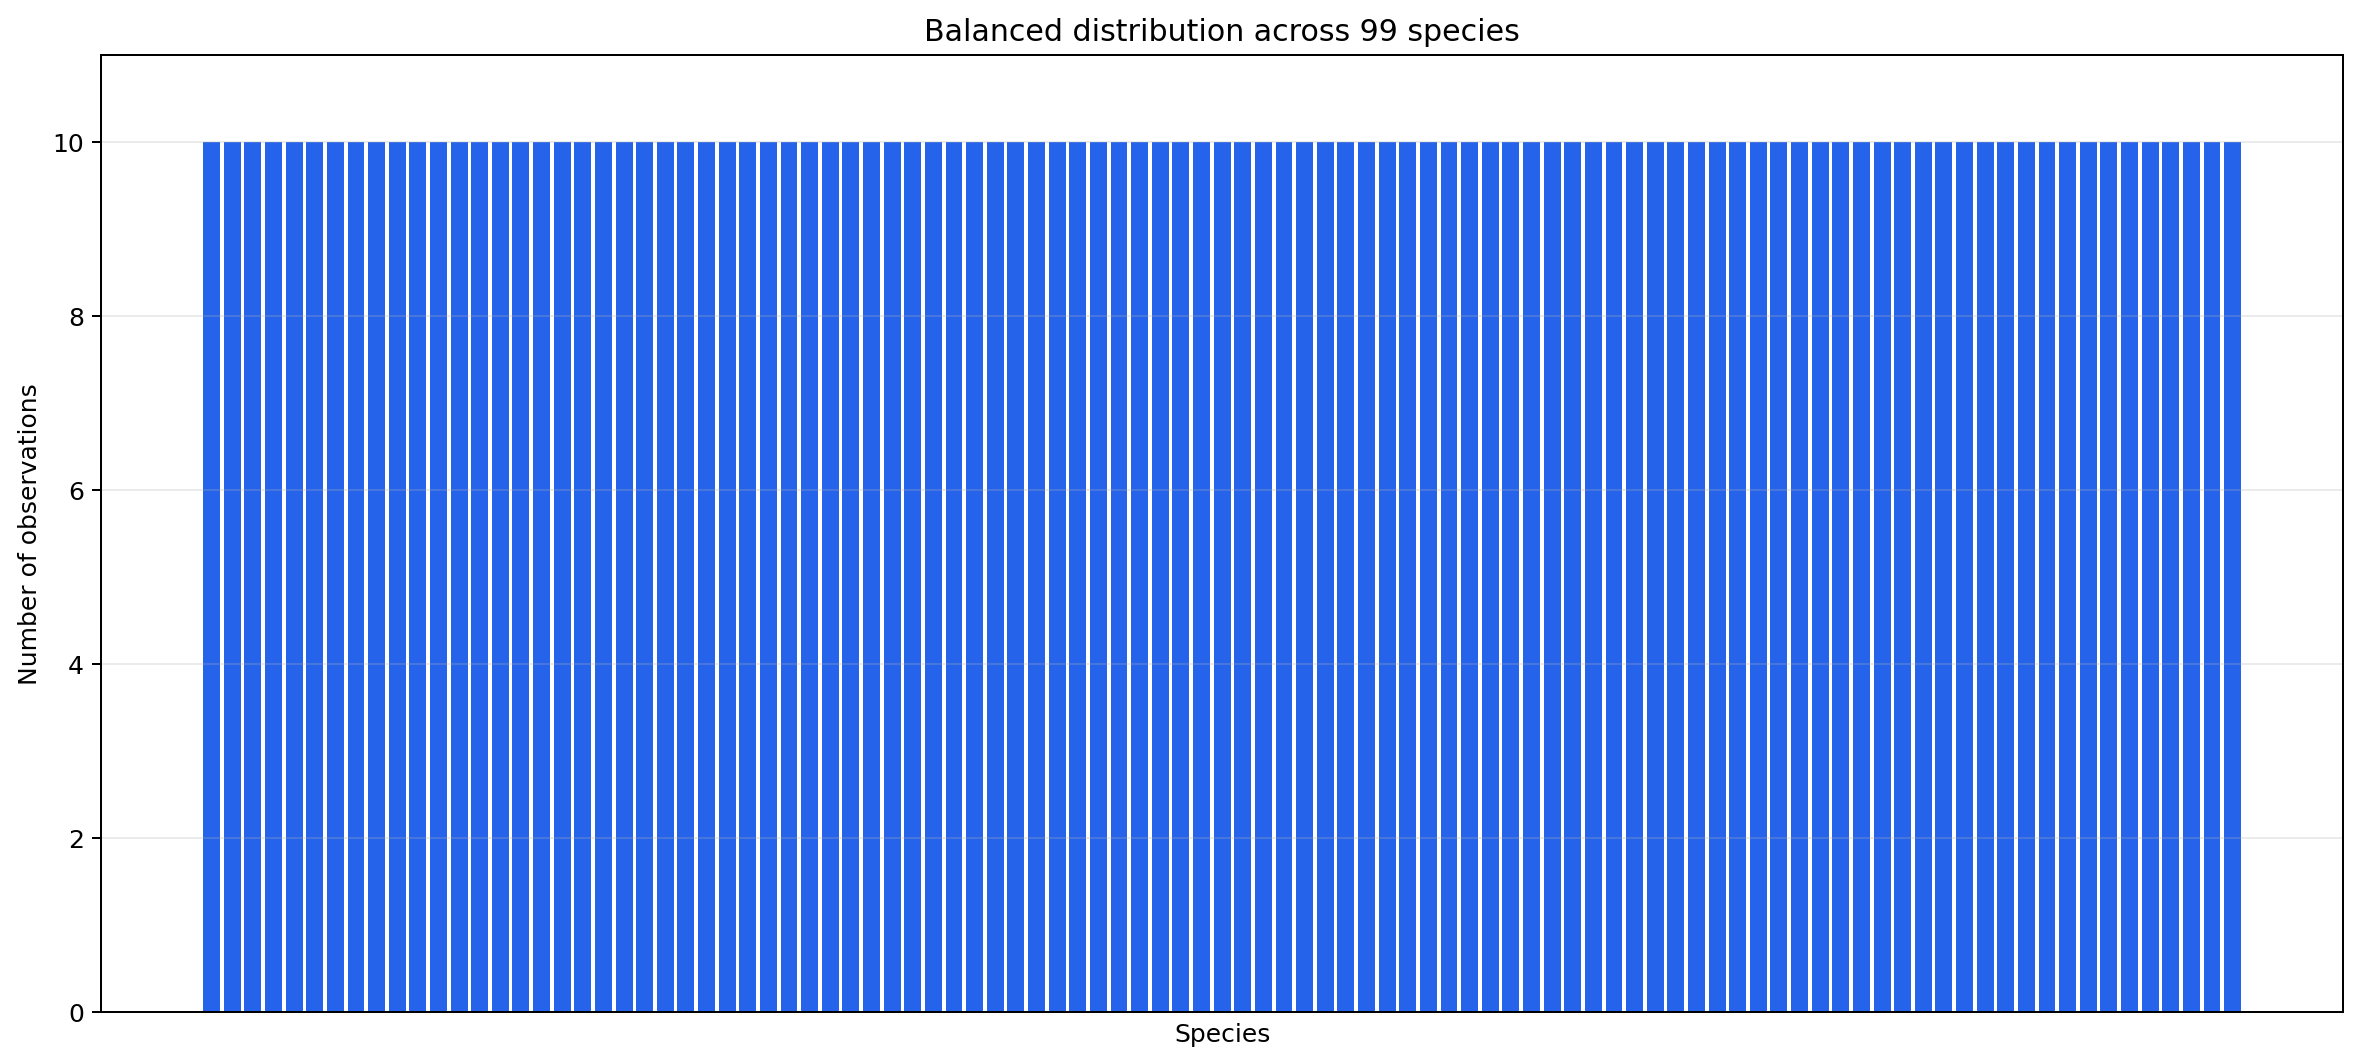
\includegraphics[width=\textwidth]{../figures/en/fig01_distribution_classes.png}
\caption{Number of observations per species. The uniform bar heights confirm that the training sample has no class imbalance.}
\end{figure}

\subsection{Feature scale, dispersion, and distributional shape}
The marginal distributions show that the three feature families operate on different scales. The \texttt{shape} variables occupy a very narrow range, with a mean standard deviation of \texttt{0.00029}, whereas the \texttt{margin} and \texttt{texture} variables have mean standard deviations of \texttt{0.01688} and \texttt{0.02696}, respectively. This scale heterogeneity is scientifically important because it directly affects methods that are sensitive to feature norms or to the geometry of the point cloud.

Boxplots play a central role here. Unlike a simple table of means, they simultaneously show the median, interquartile spread, skewness, and extreme values. In this dataset, they indicate that the \texttt{texture} family has the greatest dispersion, whereas \texttt{shape} is much more tightly concentrated. This observation does not establish that standardization will necessarily improve every learning procedure, but it provides a strong descriptive rationale for examining scaled variants.

\begin{table}[H]
\centering
\small
\begin{tabular}{|l|r|r|r|r|r|r|r|}
\hline
\textbf{Family} & \textbf{Min} & \textbf{Max} & \textbf{Mean Q1} & \textbf{Mean median} & \textbf{Mean Q3} & \textbf{Mean of means} & \textbf{Mean std. dev.} \\
\hline
\texttt{margin} & \texttt{0.00000} & \texttt{0.38867} & \texttt{0.00354} & \texttt{0.01028} & \texttt{0.02237} & \texttt{0.01562} & \texttt{0.01688} \\
\texttt{shape} & \texttt{0.00002} & \texttt{0.00301} & \texttt{0.00041} & \texttt{0.00056} & \texttt{0.00073} & \texttt{0.00061} & \texttt{0.00029} \\
\texttt{texture} & \texttt{0.00000} & \texttt{0.85352} & \texttt{0.00072} & \texttt{0.00543} & \texttt{0.01871} & \texttt{0.01563} & \texttt{0.02696} \\
\hline
\end{tabular}
\caption{Descriptive statistics by feature family}
\end{table}

\begin{figure}[H]
\centering
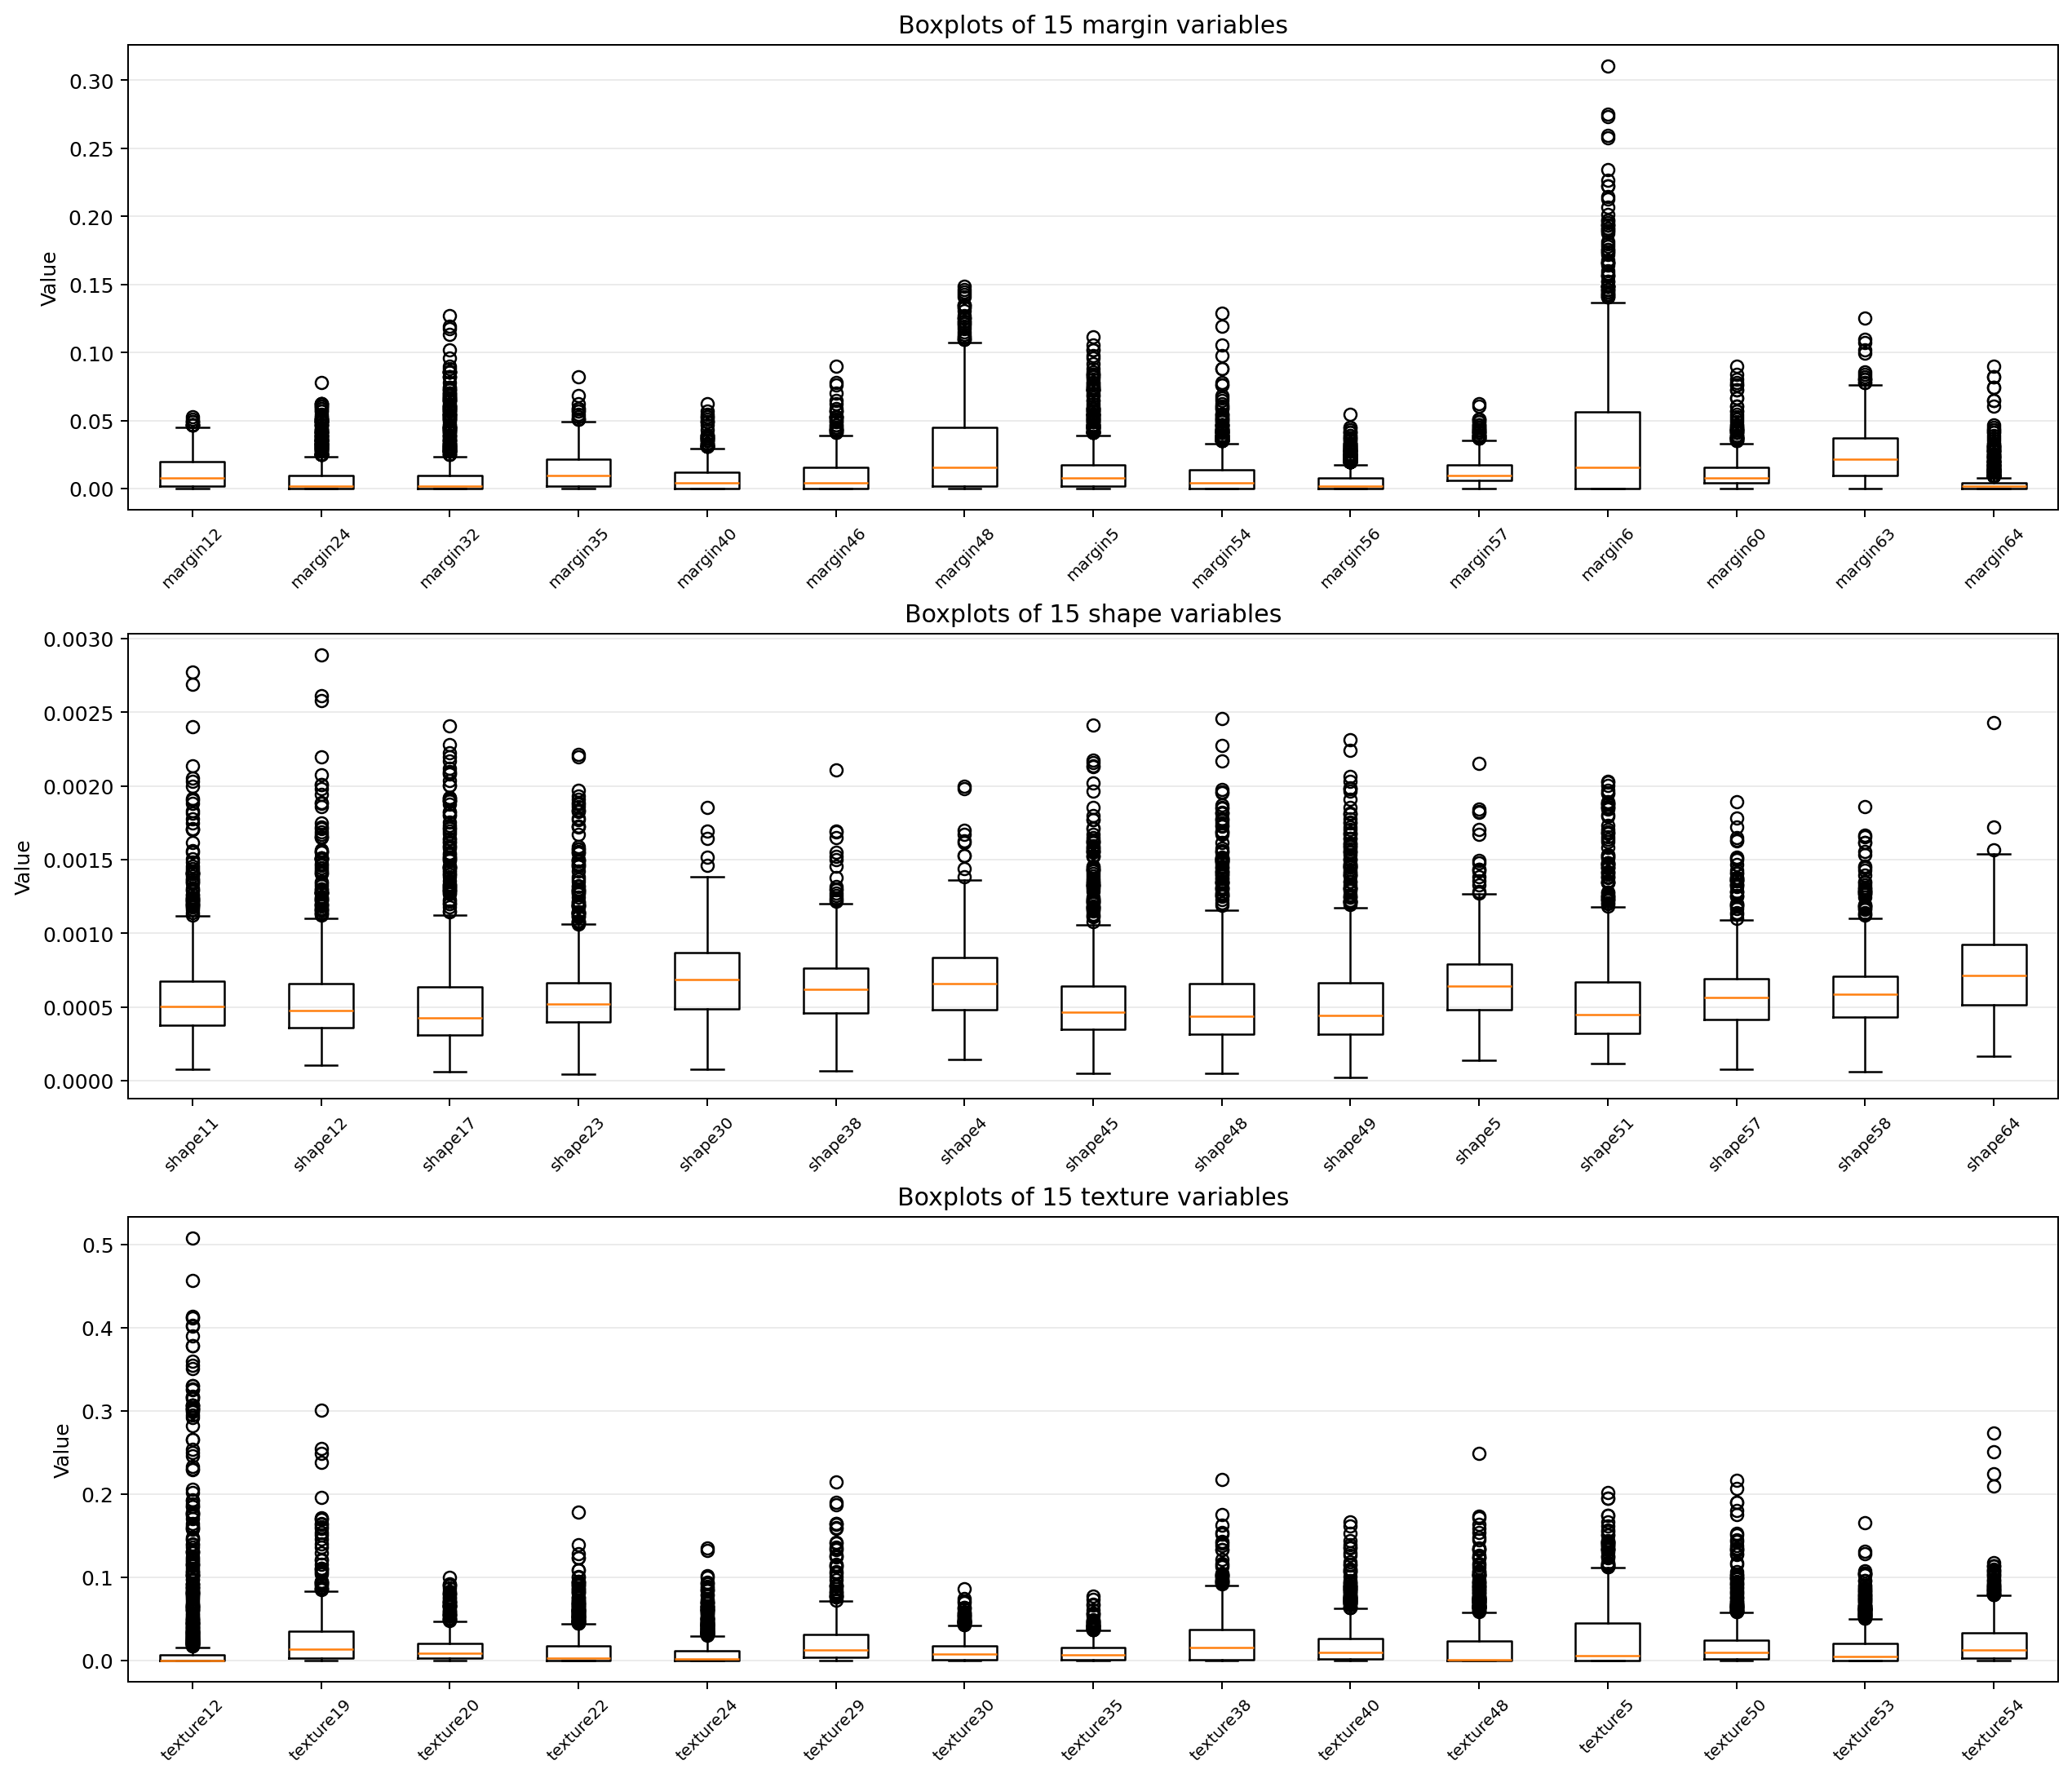
\includegraphics[width=\textwidth]{../figures/en/figA11_boxplots_variables.png}
\caption{Boxplots of selected variables from the \texttt{margin}, \texttt{shape}, and \texttt{texture} families. The visual comparison highlights scale heterogeneity and the greater dispersion of the texture variables.}
\end{figure}

The shape of the distributions supports this interpretation. The mean absolute skewness of the \texttt{192} variables is approximately \texttt{2.20}, with a maximum close to \texttt{10.91}, indicating distributions that are often asymmetric and sometimes strongly concentrated near zero. This result calls for caution when interpreting mean-based statistics alone and reinforces the value of robust descriptions based on quartiles and boxplots.

\subsection{Correlations and redundancy among descriptors}
The correlation matrix reveals a clear block structure. The \texttt{shape} family is by far the most redundant, with a mean absolute within-family correlation of \texttt{0.6996}, compared with \texttt{0.2606} for \texttt{margin} and \texttt{0.1612} for \texttt{texture}. Between-family dependencies remain weak, ranging from \texttt{0.0548} to \texttt{0.0781}, suggesting that the three families do not capture exactly the same descriptive information.

\begin{table}[H]
\centering
\begin{tabular}{|l|r|}
\hline
\textbf{Block} & \textbf{Mean absolute correlation} \\
\hline
\texttt{shape-shape} & \texttt{0.6996} \\
\texttt{margin-margin} & \texttt{0.2606} \\
\texttt{texture-texture} & \texttt{0.1612} \\
\texttt{margin-shape} & \texttt{0.0675} \\
\texttt{margin-texture} & \texttt{0.0781} \\
\texttt{shape-texture} & \texttt{0.0548} \\
\hline
\end{tabular}
\caption{Mean absolute within- and between-family correlation}
\end{table}

\begin{table}[H]
\centering
\begin{tabular}{|c|l|r|}
\hline
\textbf{Rank} & \textbf{Pair} & \textbf{Correlation} \\
\hline
1 & \texttt{shape49} - \texttt{shape50} & \texttt{0.9939} \\
2 & \texttt{shape17} - \texttt{shape18} & \texttt{0.9939} \\
3 & \texttt{shape15} - \texttt{shape16} & \texttt{0.9937} \\
4 & \texttt{shape16} - \texttt{shape17} & \texttt{0.9936} \\
5 & \texttt{shape18} - \texttt{shape19} & \texttt{0.9936} \\
\hline
\end{tabular}
\caption{Most highly correlated variable pairs}
\end{table}

In total, \texttt{445} variable pairs have an absolute correlation of at least \texttt{0.90}, and \texttt{197} have a correlation of at least \texttt{0.95}. These magnitudes justify examining dimensionality reduction with \texttt{PCA}, without presuming that it will benefit the subsequent learning stages.

\begin{figure}[H]
\centering
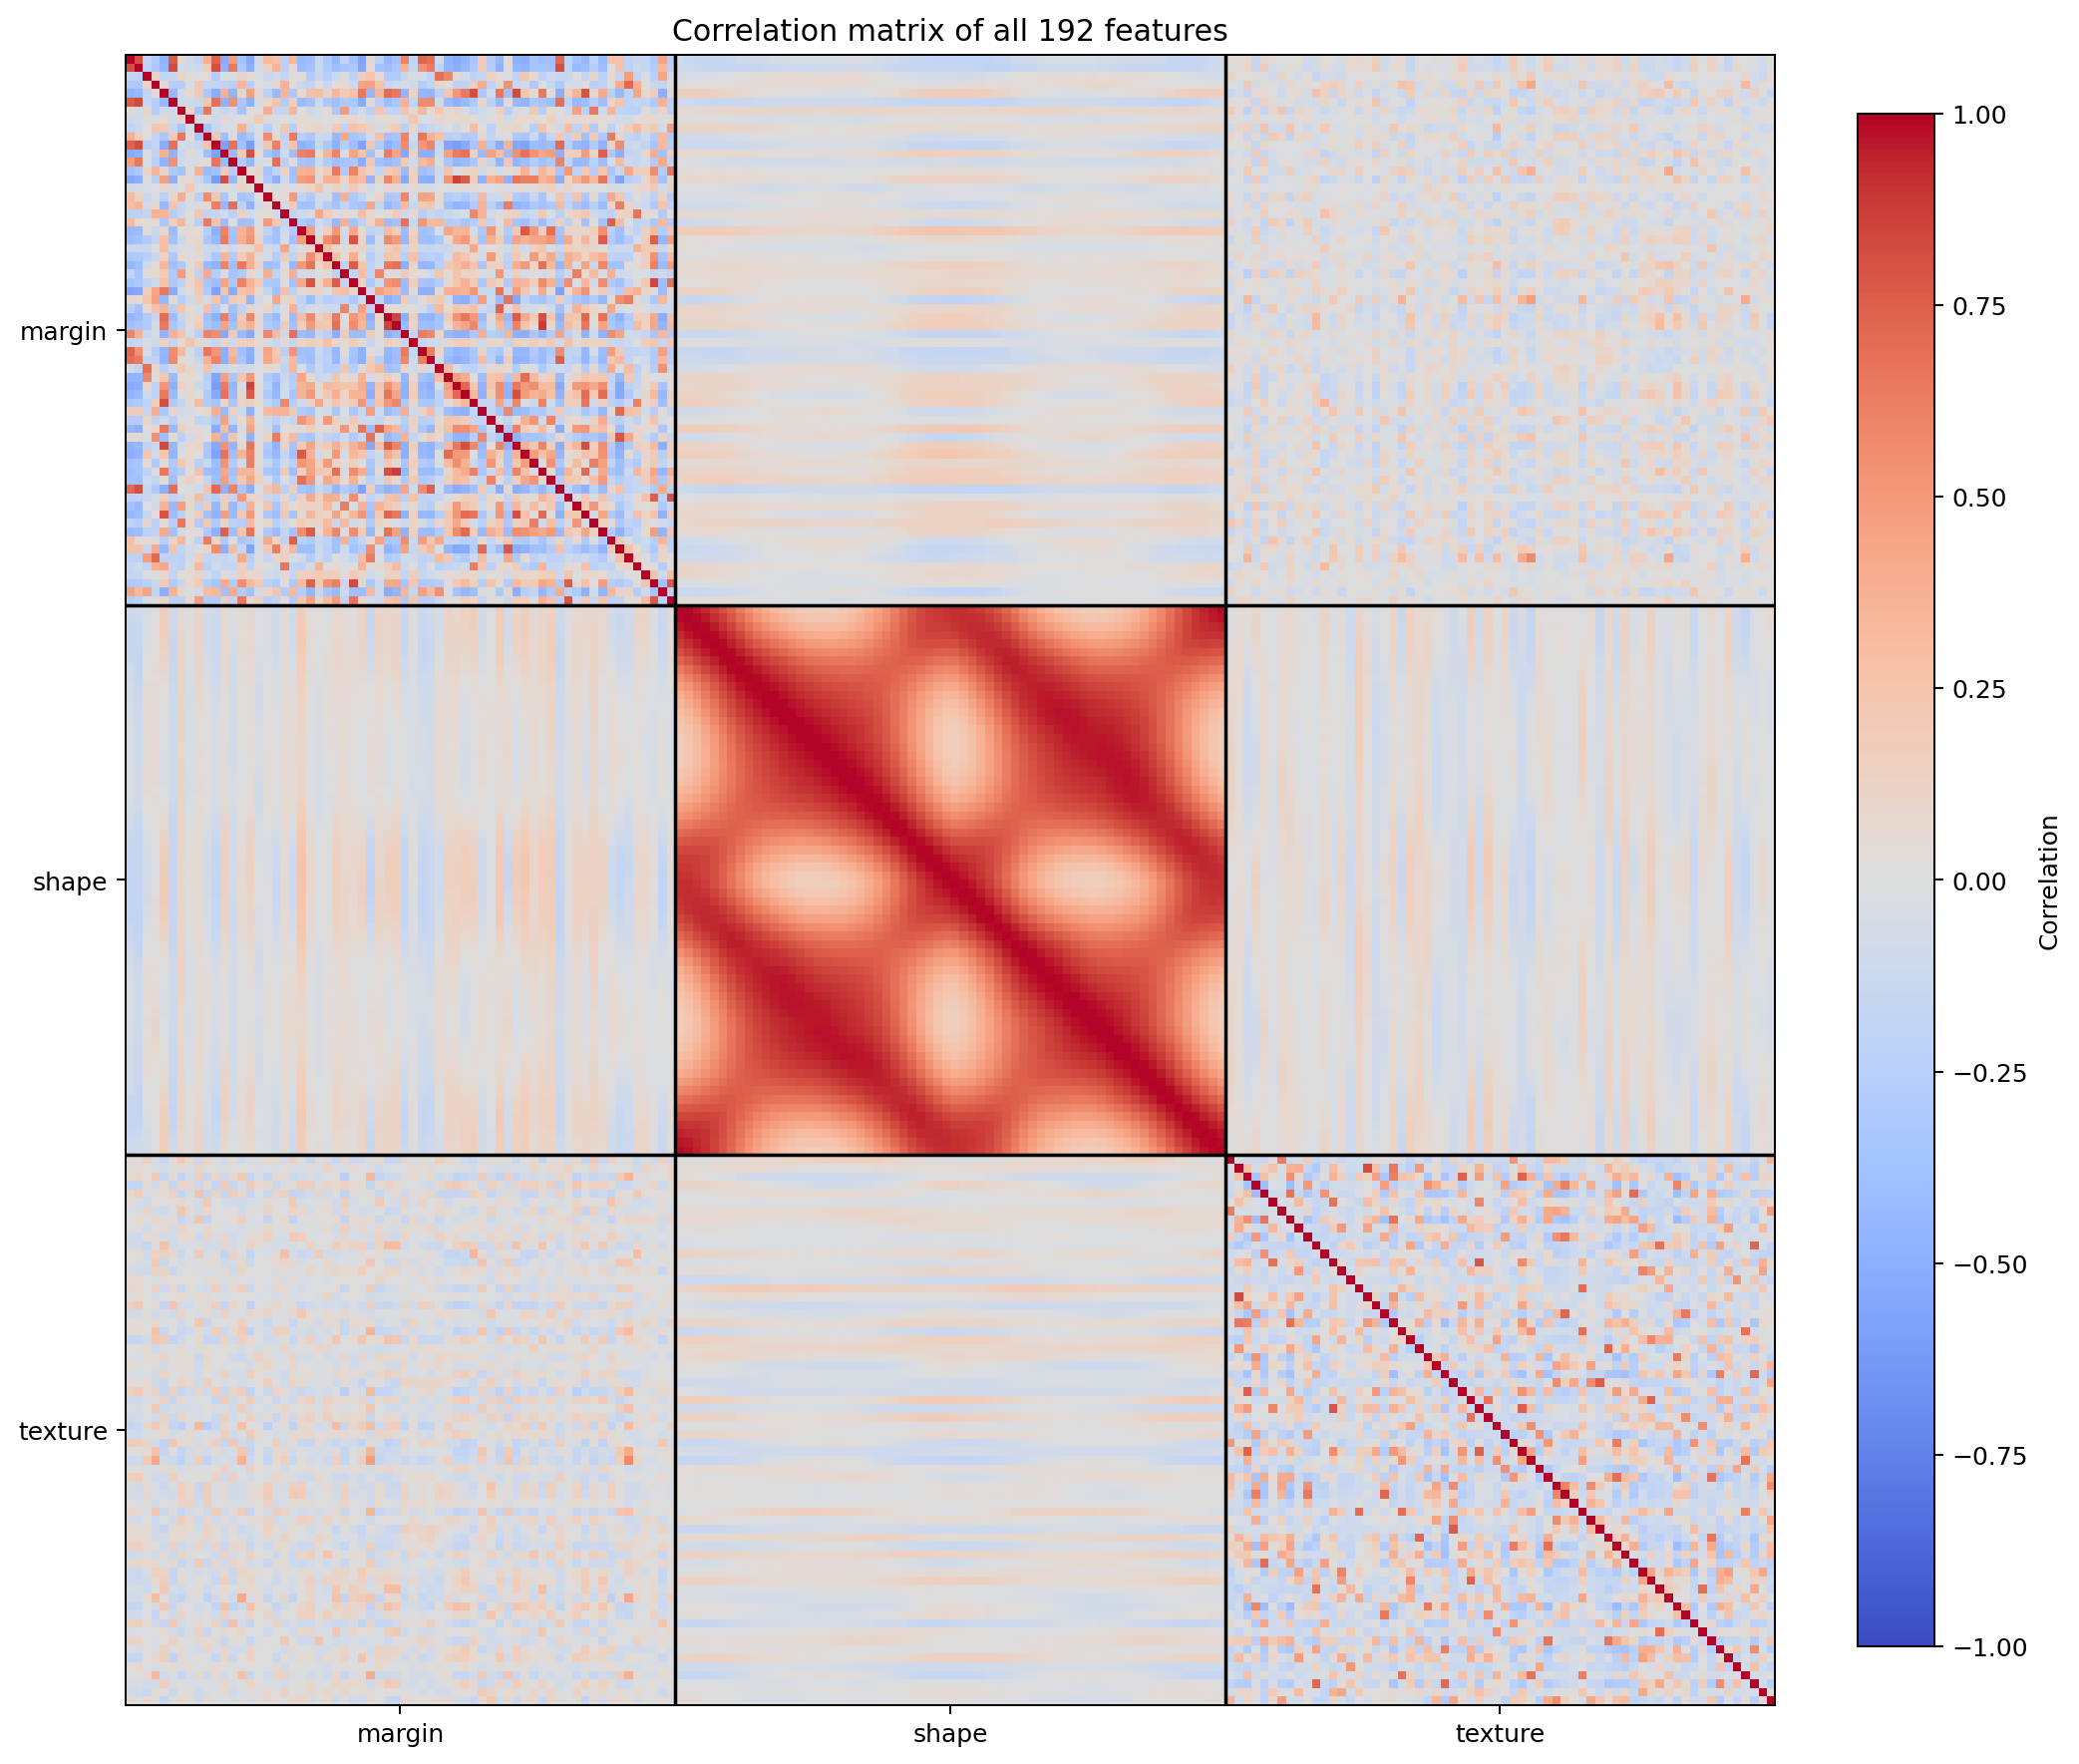
\includegraphics[width=\textwidth]{../figures/en/figA12_heatmap_correlation.png}
\caption{Correlation matrix for the \texttt{192} variables. The block structure reveals particularly strong internal redundancy within the \texttt{shape} family, while relationships between families remain weaker.}
\end{figure}

\subsection{Dimensionality reduction and global organization}
\texttt{PCA} was applied to the standardized data to summarize the dataset's linear structure. The first two components explain approximately \texttt{24.2 \%} and \texttt{10.4 \%} of the total variance, or just under \texttt{34.6 \%} combined. The first five components account for \texttt{50.7 \%}, and the first ten for \texttt{64.7 \%}. The reduction is therefore meaningful, but not radical enough to suggest that a very low-dimensional space would adequately summarize the information.

The cumulative variance thresholds reinforce this interpretation. It takes \texttt{23} components to reach \texttt{80 \%} explained variance, \texttt{44} to reach \texttt{90 \%}, \texttt{69} to reach \texttt{95 \%}, and \texttt{116} to reach \texttt{99 \%}. Thus, \texttt{PCA} is defensible as a tool for moderate compression and mitigation of linear redundancy, but not as a drastic reduction of the problem.

\begin{table}[H]
\centering
\begin{tabular}{|l|r|}
\hline
\textbf{Cumulative explained variance} & \textbf{Number of components} \\
\hline
\texttt{80 \%} & \texttt{23} \\
\texttt{90 \%} & \texttt{44} \\
\texttt{95 \%} & \texttt{69} \\
\texttt{99 \%} & \texttt{116} \\
\hline
\end{tabular}
\caption{Number of components required at different variance thresholds}
\end{table}

\begin{figure}[H]
\centering
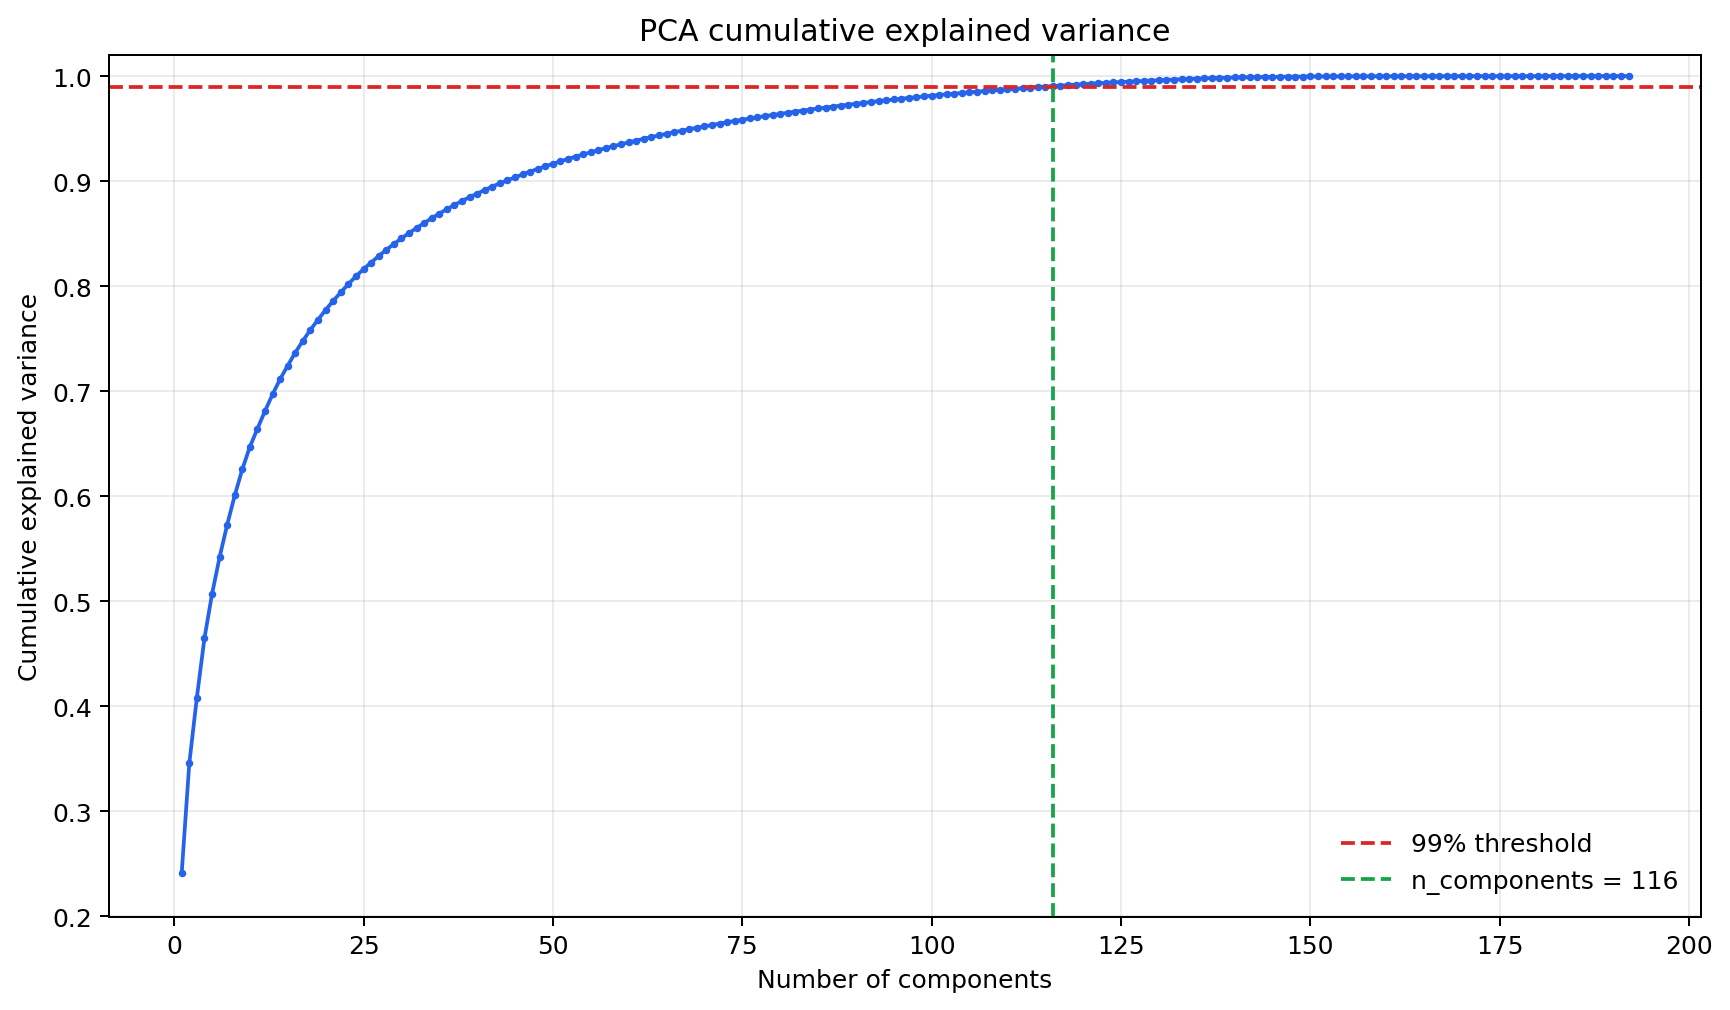
\includegraphics[width=\textwidth]{../figures/en/figA13_pca_variance_cumulative.png}
\caption{Cumulative explained variance after standardization. The curve's gradual increase indicates that much of the information can be compressed, but that a substantial number of components is still required to retain nearly all variance.}
\end{figure}

The two-dimensional \texttt{t-SNE} projection complements this linear view. In the notebook, it is computed after an initial \texttt{PCA} reduction to \texttt{50} components, with a perplexity of \texttt{30}. Its purpose is not to summarize variance quantitatively, but to examine the local consistency of neighborhoods among observations. The figure reveals partial groupings alongside overlapping regions, suggesting exploitable structure without implying trivial separation of the \texttt{99} species in a very low-dimensional space.

This interpretation must remain cautious. \texttt{t-SNE} primarily preserves local proximity relationships and depends on its hyperparameters; it provides neither a measure of global separability nor sufficient evidence to favor a particular preprocessing method. Its value here is heuristic: it confirms organization in the point cloud beyond pure noise without establishing the exact difficulty of the task.

\begin{figure}[H]
\centering
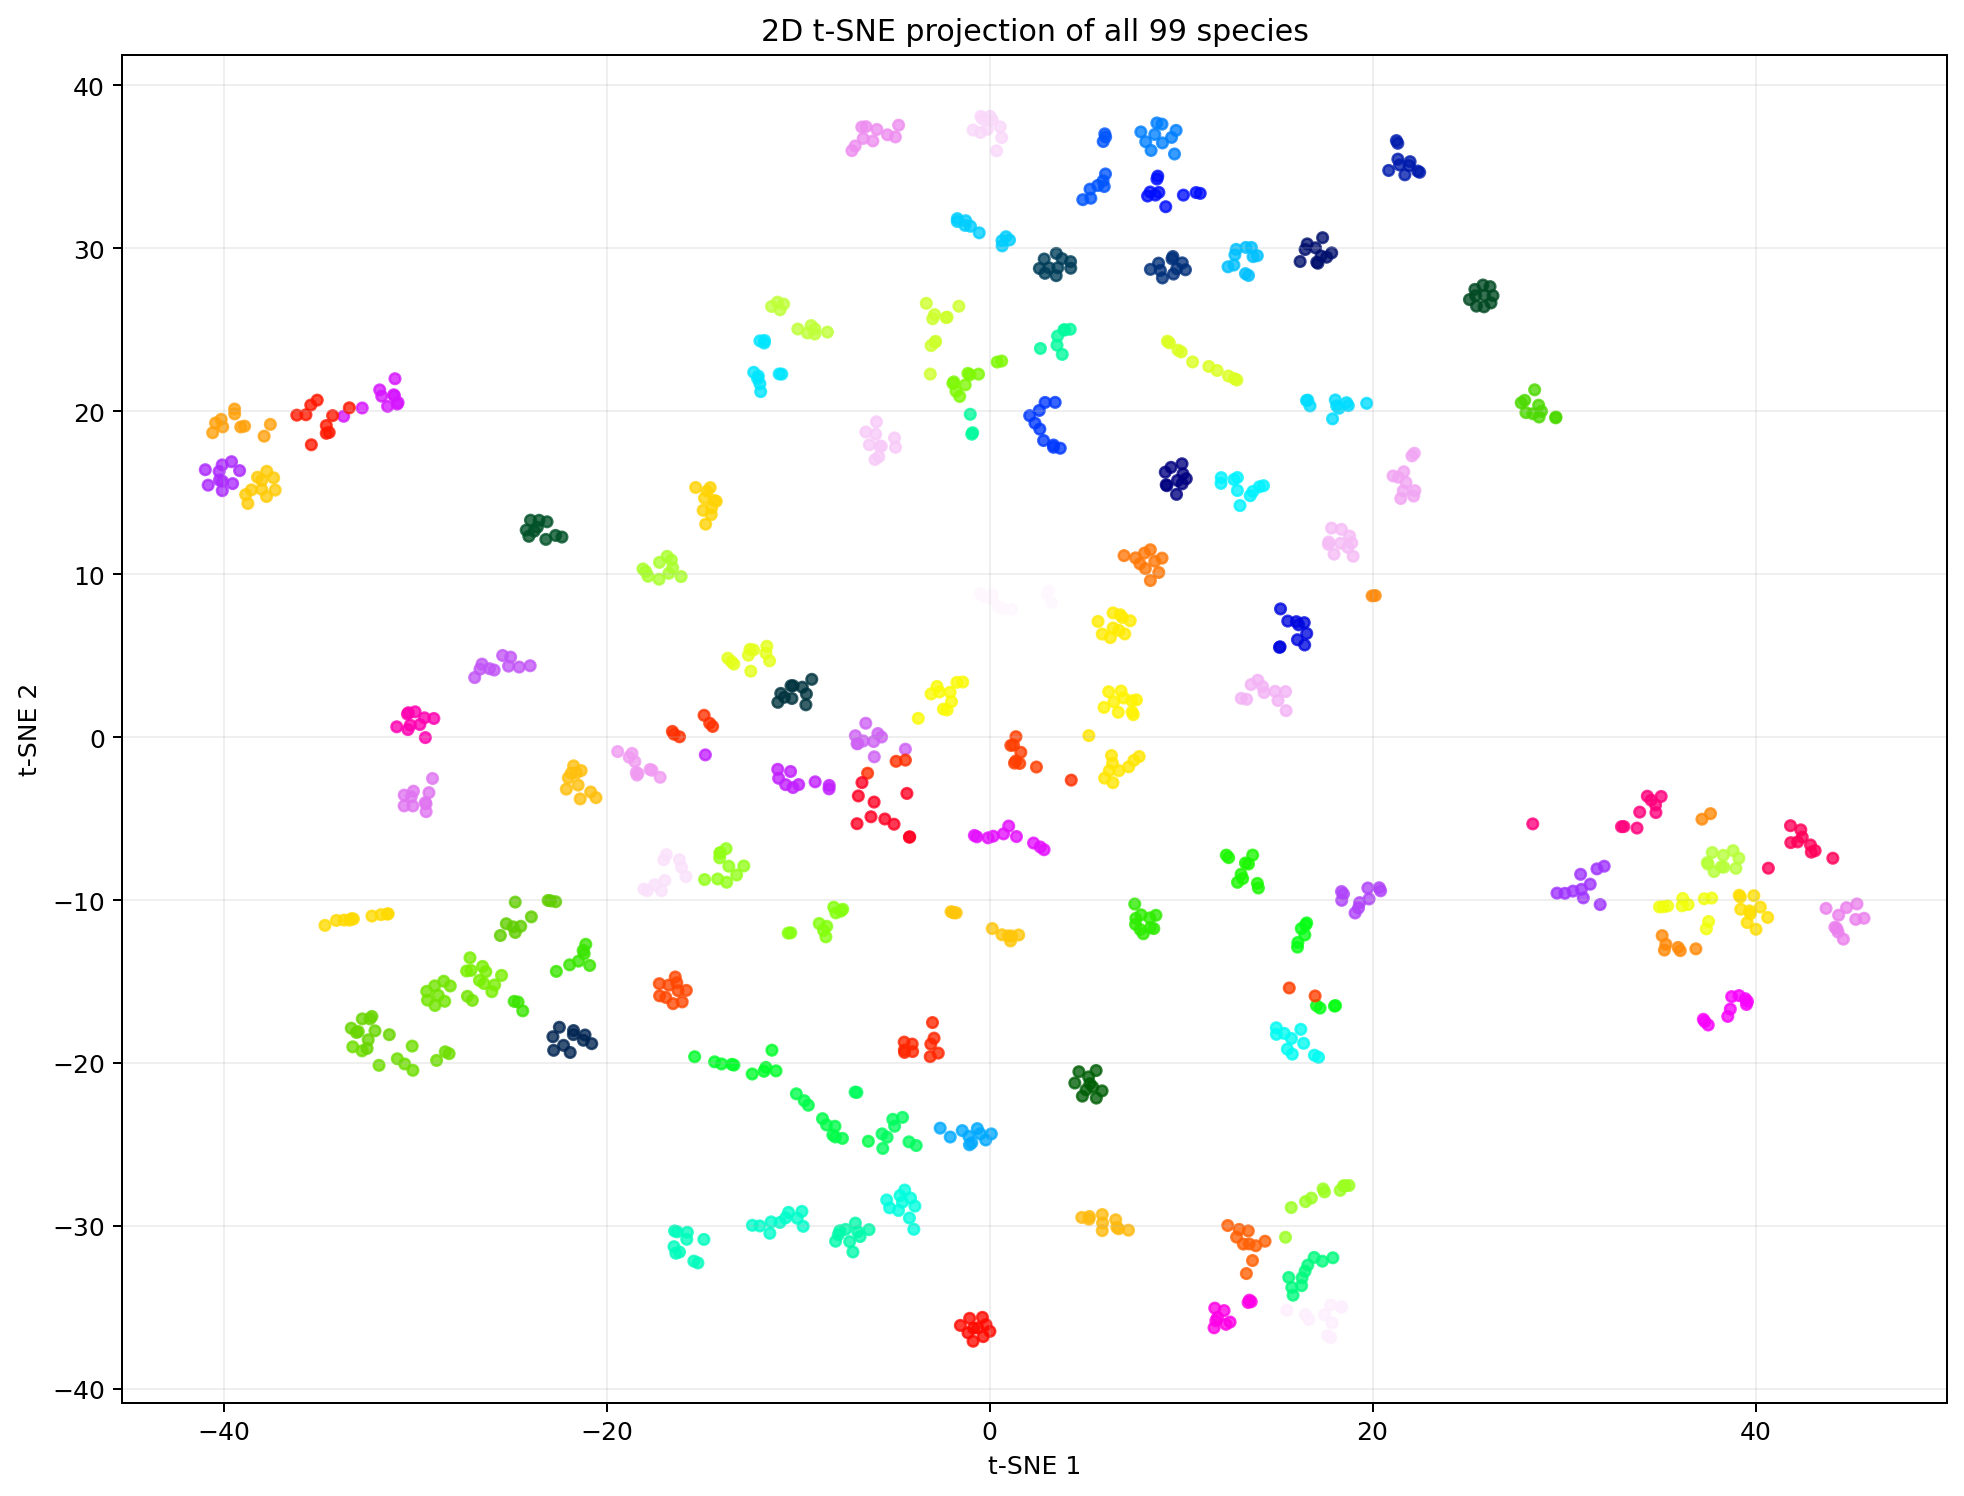
\includegraphics[width=\textwidth]{../figures/en/figA14_tsne_2d.png}
\caption{\texttt{t-SNE} 2D projection of the \texttt{99} species after standardization and an initial \texttt{PCA} reduction. Local clusters coexist with substantial overlap, consistent with a learnable problem that is far from trivial.}
\end{figure}

\subsection{Methodological implications and summary}
Four lessons emerge from this exploratory analysis. First, the dataset is structurally sound and perfectly balanced, but remains sparse at the species level, calling for restraint when interpreting variations observed on small subsets. Second, the differences in scale and dispersion among feature families provide a strong descriptive motivation for examining standardization procedures. Third, the pronounced redundancy, especially within \texttt{shape}, makes the study of \texttt{PCA} as a linear compression method methodologically plausible. Fourth, the reduced-dimensional projections indicate exploitable structure while emphasizing that this structure is not equivalent to simple separability.

Consequently, the preprocessing choices examined later can be scientifically motivated by this EDA, but they remain hypotheses at this stage. Standardization and \texttt{PCA} are reasonable exploratory options, not guarantees of improvement.

\subsection{Protocol safeguards for the subsequent analysis}
The preceding descriptive findings justify a cautious protocol for model comparison. The dataset is balanced, but each species remains sparsely represented; it would therefore be methodologically risky to combine variant selection, tuning, and final evaluation on the same subset. For this reason, the remainder of the report explicitly distinguishes exploration, confirmation, and secondary corroboration.

\begin{table}[H]
\centering
\begin{tabular}{|l|l|}
\hline
\textbf{Element} & \textbf{Selected value} \\
\hline
Frozen split & \texttt{80 \%} development / \texttt{20 \%} corroboration \\
Development-set size & \texttt{792} \\
Corroboration-set size & \texttt{198} \\
Primary cross-validation & \texttt{5} outer folds \\
Inner tuning & \texttt{3} inner folds \\
Primary metric & \texttt{F1-macro} \\
Secondary metric & \texttt{Accuracy} \\
Global seed & \texttt{42} \\
Status of non-\texttt{tuned} variants & \texttt{Exploratory} \\
Status of \texttt{tuned} variants & \texttt{Confirmatory} \\
Status of corroboration set & \texttt{Secondary corroboration} \\
\hline
\end{tabular}
\caption{Safeguards in the experimental protocol}
\end{table}

This evidence hierarchy guides the reading of all subsequent sections. The non-\texttt{tuned} variants document the effects of preprocessing and tuning, the \texttt{tuned} results determine the primary ranking, and the frozen corroboration set is used only for secondary verification.

% ==========================================
% 3. MODEL STUDY
% ==========================================

\section{Model study}

This section compares six model families under a strictly common experimental framework. The primary metric is \texttt{F1-macro}, selected to give equal weight to all \texttt{99} species, while \texttt{accuracy} serves as the secondary metric.

The analysis follows three clearly distinguished levels of evidence. Exploratory variants use simple cross-validation to measure the effects of preprocessing or complexity control. The primary result for each family is the \texttt{tuned} variant, evaluated through nested cross-validation. When available, secondary corroboration on the frozen split is used solely to determine whether the signal observed on the development set persists on data never seen during modeling.

The following subsections share a common structure. Each model is first situated within the scientific rationale of the study, then examined from exploratory, confirmatory, and, where available, secondary corroboration perspectives.

The purpose of this section is not yet to reach an overall verdict among models, but to understand how each family responds to preprocessing, complexity control, and tuning. The cross-model synthesis is deliberately reserved for the next section to maintain a clear separation between family-specific analysis and the final comparative assessment.

% --- PERCEPTRON ---
\subsection{Perceptron model}

\subsubsection{Role of the model}
The perceptron is the study's minimal linear baseline. Its purpose is less to compete with the best models than to quantify what an elementary decision boundary can extract from a high-dimensional multiclass problem. It therefore provides a useful reference point for measuring the effect of standardization and, more generally, the need for additional model capacity.

\subsubsection{Exploration}
The exploratory stage immediately shows that preprocessing plays a central role for this family. The raw variant achieves a \texttt{F1-macro} of \texttt{0.6979} and an \texttt{accuracy} of \texttt{0.7436}. Adding \texttt{StandardScaler} raises \texttt{F1-macro} to \texttt{0.8228}, while the \texttt{scaled\_pca} variant reaches \texttt{0.8057}. The main gain therefore comes from scaling; dimensionality reduction provides no additional robust improvement here.

\begin{table}[H]
\centering
\begin{tabular}{|l|l|r|r|r|r|}
\hline
\textbf{Variant} & \textbf{Protocol} & \textbf{Macro F1} & \textbf{Accuracy} & \textbf{F1 gap} & \textbf{Time (s)} \\
\hline
\texttt{default} & simple CV & \texttt{0.6979} & \texttt{0.7436} & \texttt{0.1202} & \texttt{0.62} \\
\texttt{scaled\_only} & simple CV & \texttt{0.8228} & \texttt{0.8460} & \texttt{0.1732} & \texttt{0.60} \\
\texttt{scaled\_pca} & simple CV & \texttt{0.8057} & \texttt{0.8346} & \texttt{0.1923} & \texttt{0.65} \\
\hline
\end{tabular}
\caption{Comparison of perceptron variants}
\end{table}

The perceptron therefore becomes substantially more credible after normalization, but the size of the generalization gap indicates that its room for improvement remains limited. This exploratory evidence already suggests that a low-capacity, non-probabilistic linear model will serve more as a lower bound than as a leading candidate.

\begin{figure}[H]
\centering
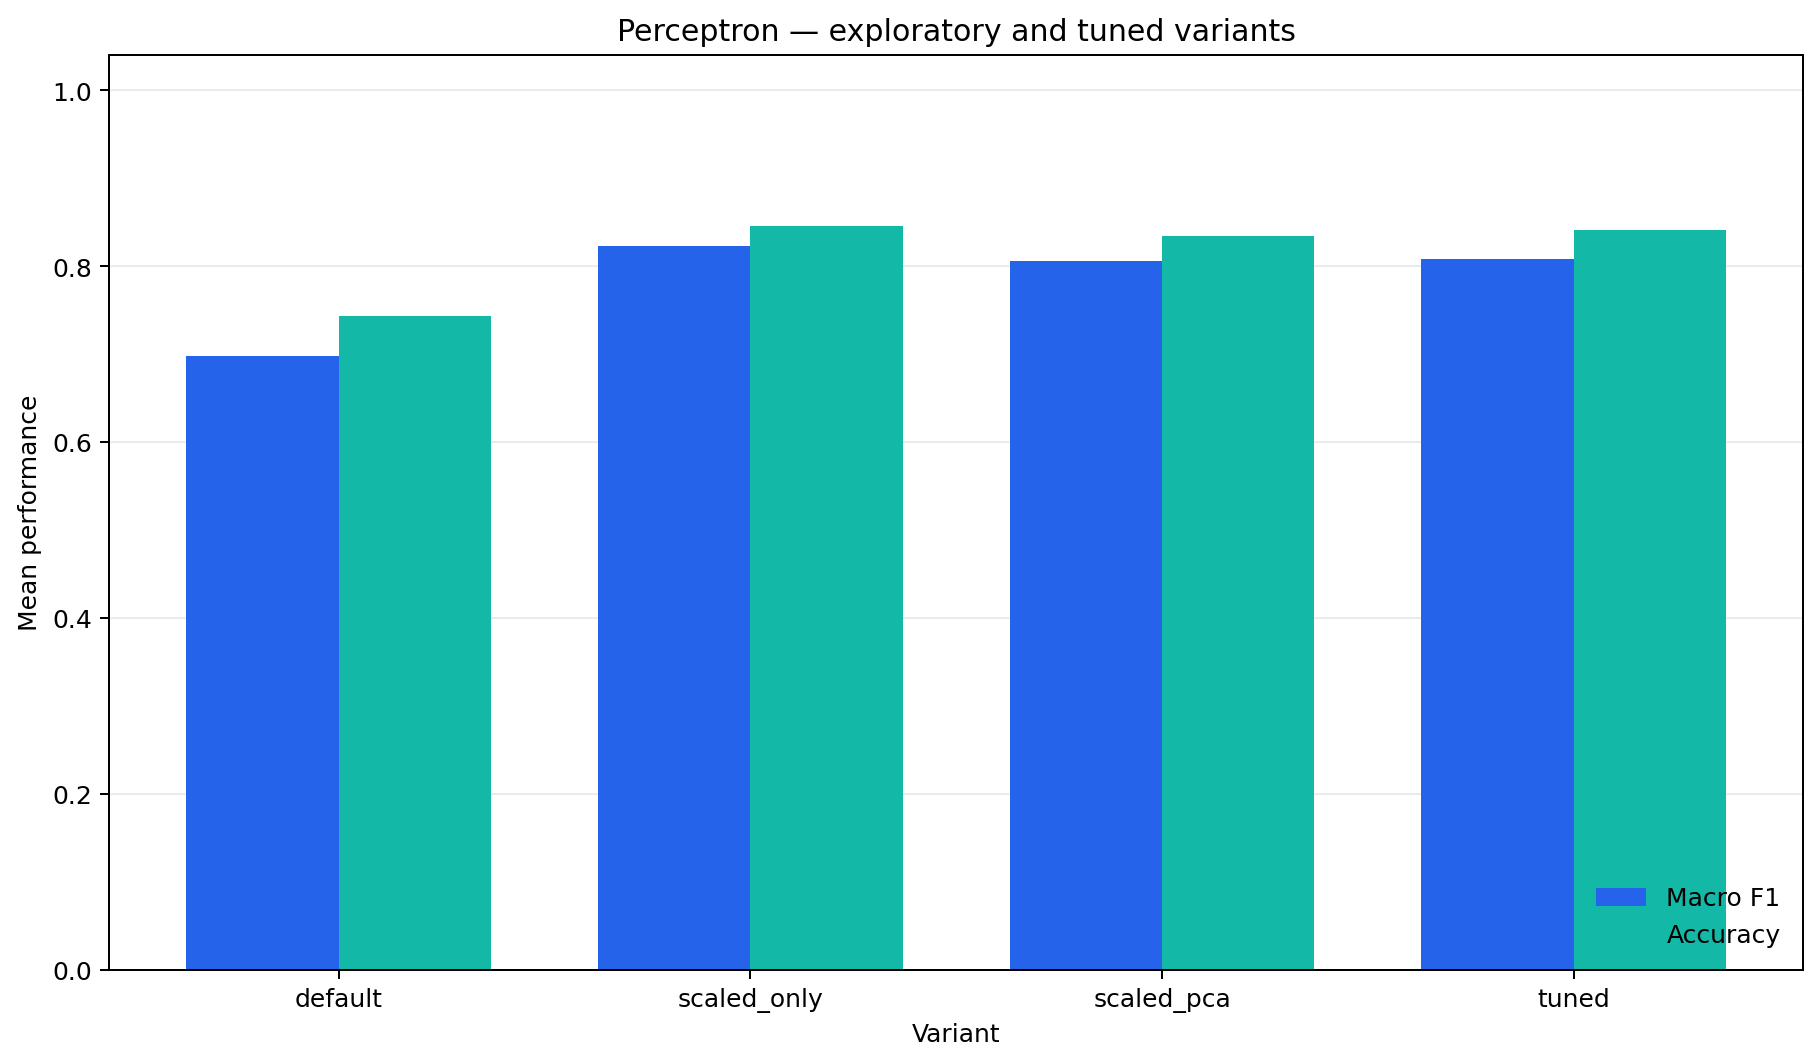
\includegraphics[width=\textwidth]{../figures/en/figA2b_comparaison_perceptron.png}
\caption{Exploratory comparison of perceptron variants. Nearly the entire performance increase is explained by feature standardization.}
\end{figure}

\subsubsection{Confirmation}
Confirmatory evaluation through nested cross-validation yields a mean \texttt{F1-macro} of \texttt{0.8085} and mean \texttt{accuracy} of \texttt{0.8409}, with standard deviations of \texttt{0.0523} and \texttt{0.0411}. The confirmatory score remains slightly below that of the best exploratory variant (\texttt{scaled\_only}), which is consistent with a less optimistic estimate after model selection.

\begin{table}[H]
\centering
\begin{tabular}{|l|r|}
\hline
\textbf{Confirmatory metric} & \textbf{Value} \\
\hline
Mean Macro F1 & \texttt{0.8085} \\
F1 standard deviation & \texttt{0.0523} \\
Mean accuracy & \texttt{0.8409} \\
Accuracy standard deviation & \texttt{0.0411} \\
Protocol & \texttt{nested CV} \\
Outer folds & \texttt{5} \\
Inner folds & \texttt{3} \\
Total time (s) & \texttt{29.79} \\
\hline
\end{tabular}
\end{table}

The scientific conclusion remains stable: once the variables are standardized, the perceptron captures a substantial part of the problem's structure, but still lags well behind the strongest families. It therefore fully serves its role as a minimal linear baseline without becoming a credible contender for the final ranking.

\subsubsection{Descriptive diagnostics}
The figures associated with the perceptron are primarily descriptive. The decision-function histogram shows the dispersion of margin scores, while the confusion matrix and leading-confusion summary show that residual errors remain relatively diffuse. This pattern is consistent with the limitations of a simple linear boundary on a problem with \texttt{99} classes.

\begin{figure}[H]
\centering
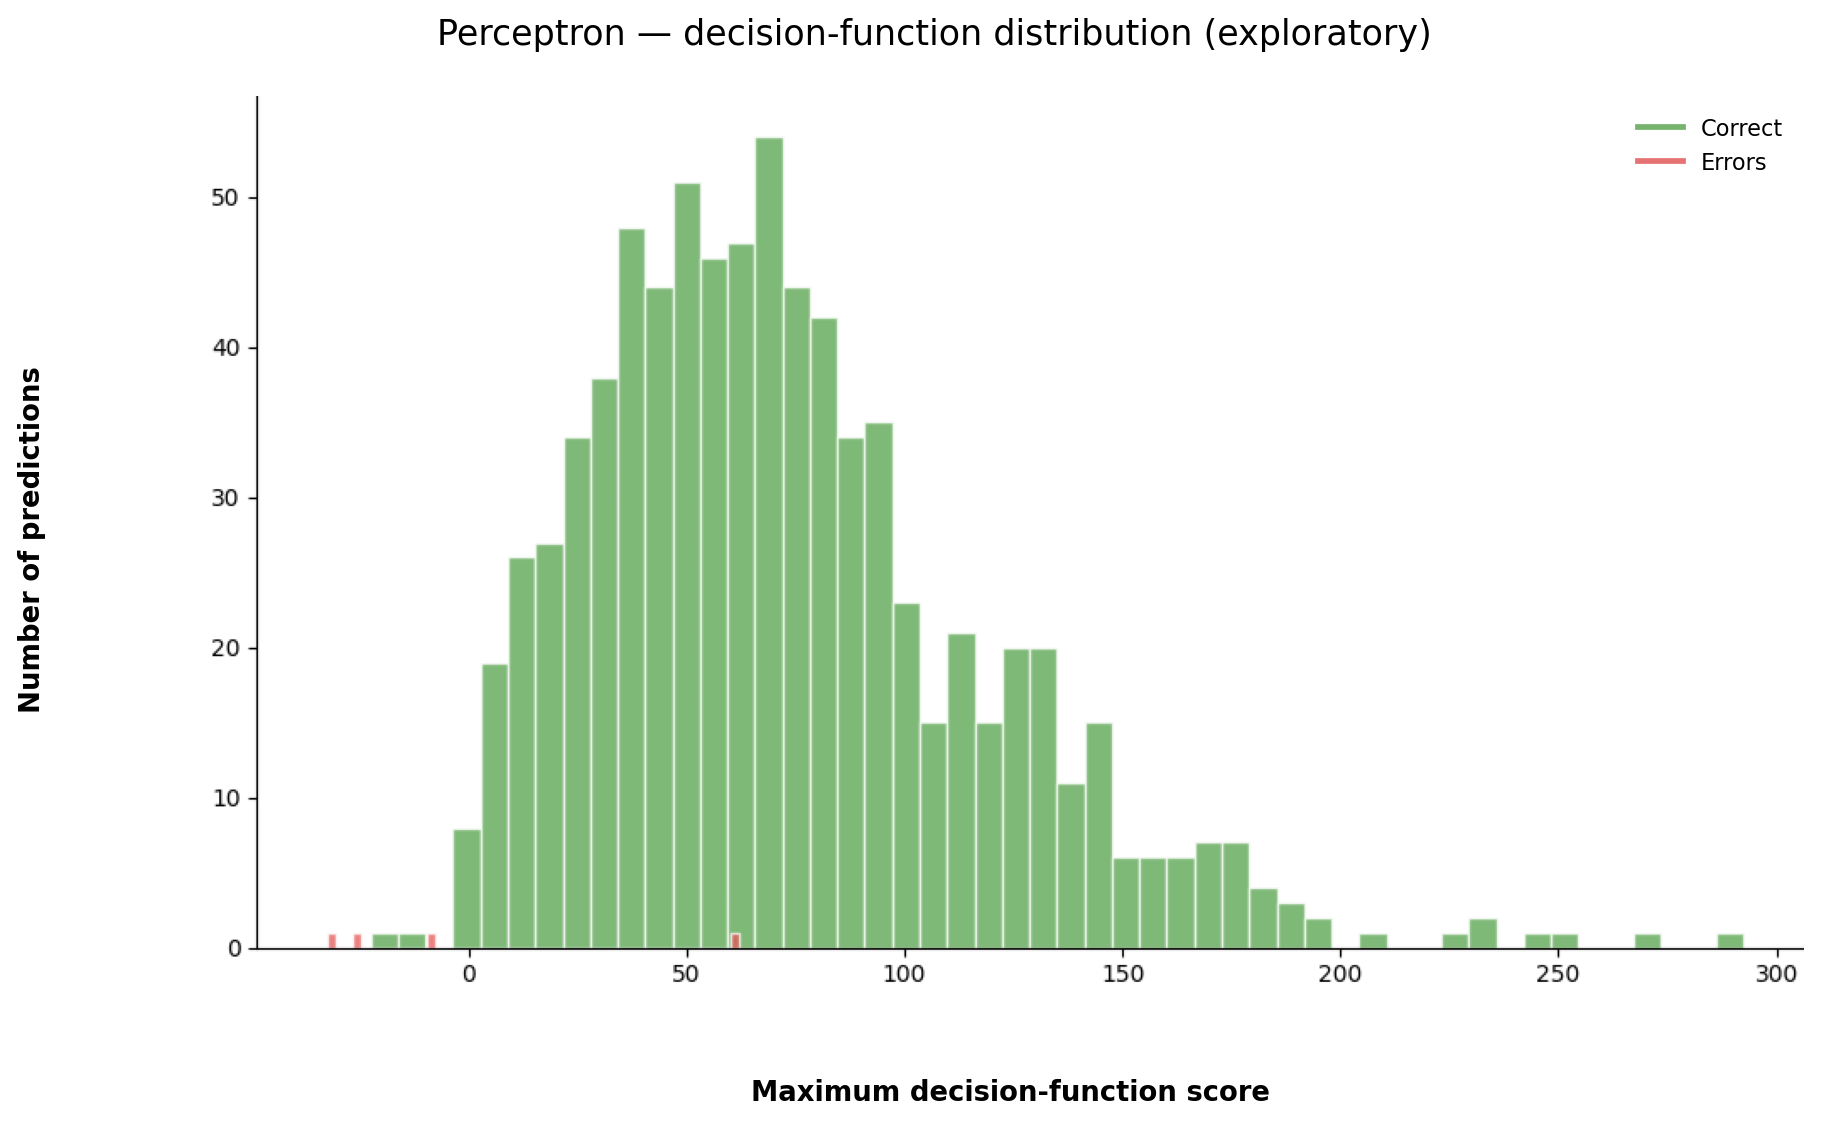
\includegraphics[width=\textwidth]{../figures/en/fig_perceptron_histogramme_fonction_decision.png}
\caption{Exploratory histogram of the perceptron's decision function. The score dispersion is consistent with a useful but still limited linear separation.}
\end{figure}

\begin{figure}[H]
\centering
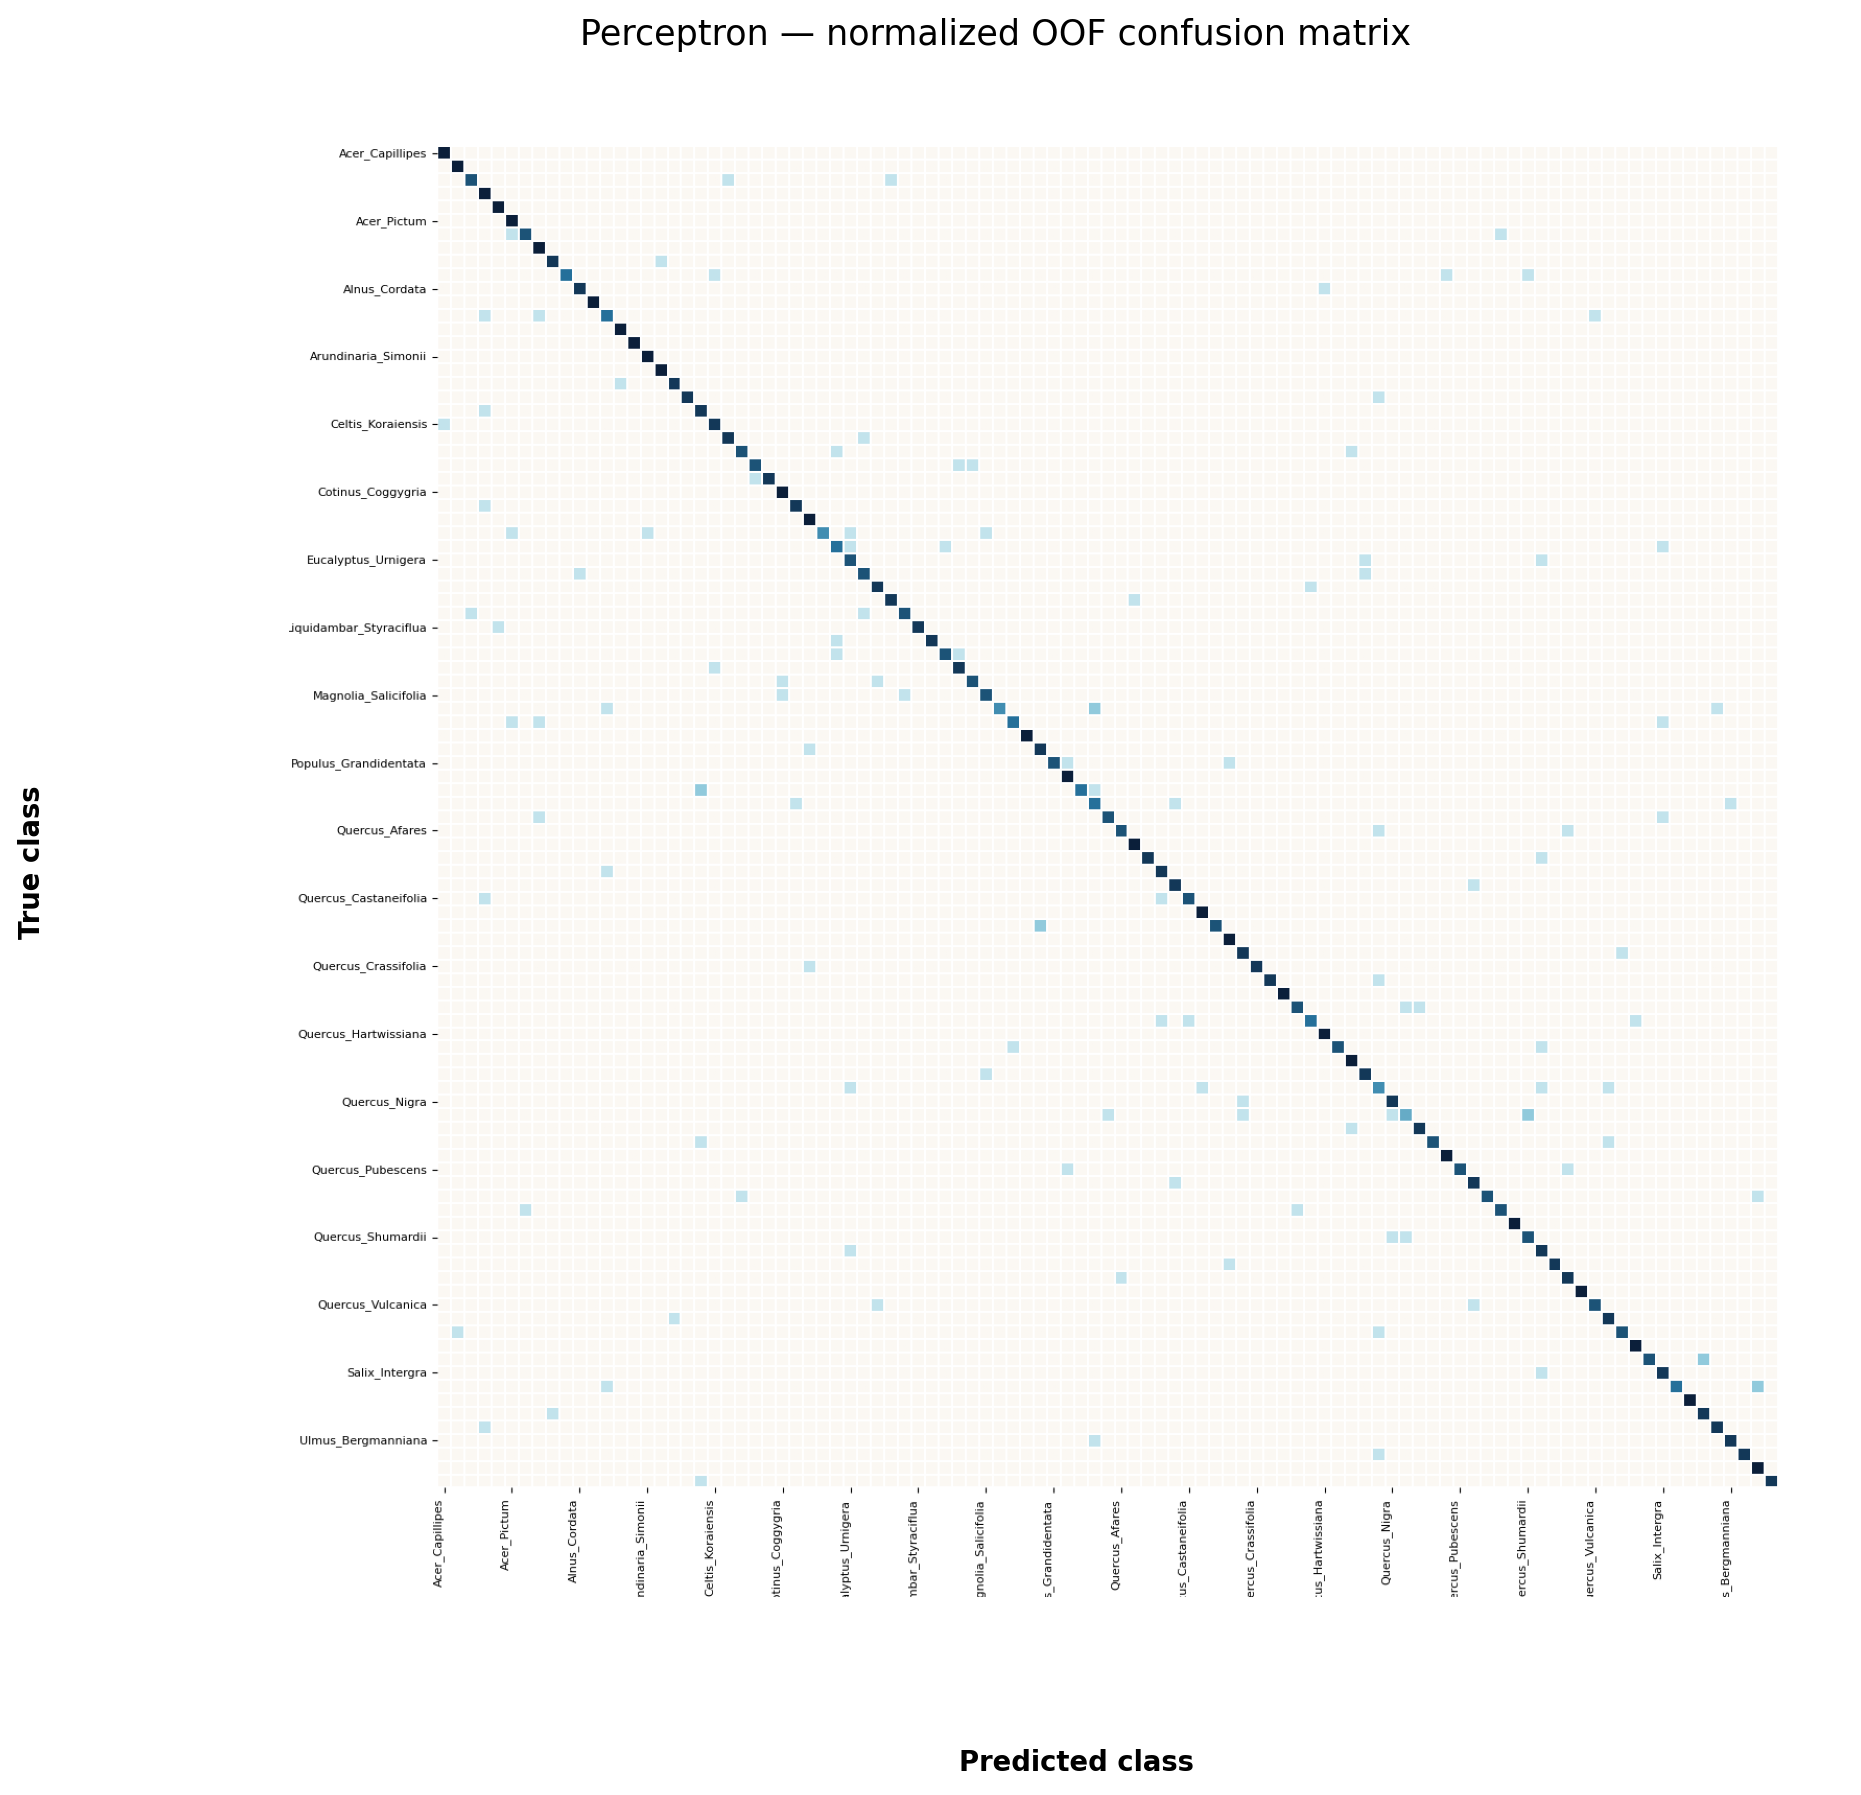
\includegraphics[width=\textwidth]{../figures/en/figA_confusion_perceptron_tuned.png}
\caption{Normalized confusion matrix obtained from the out-of-fold predictions of the \texttt{tuned} variant. Residual errors remain more diffuse than for the best-performing families.}
\end{figure}

\begin{figure}[H]
\centering
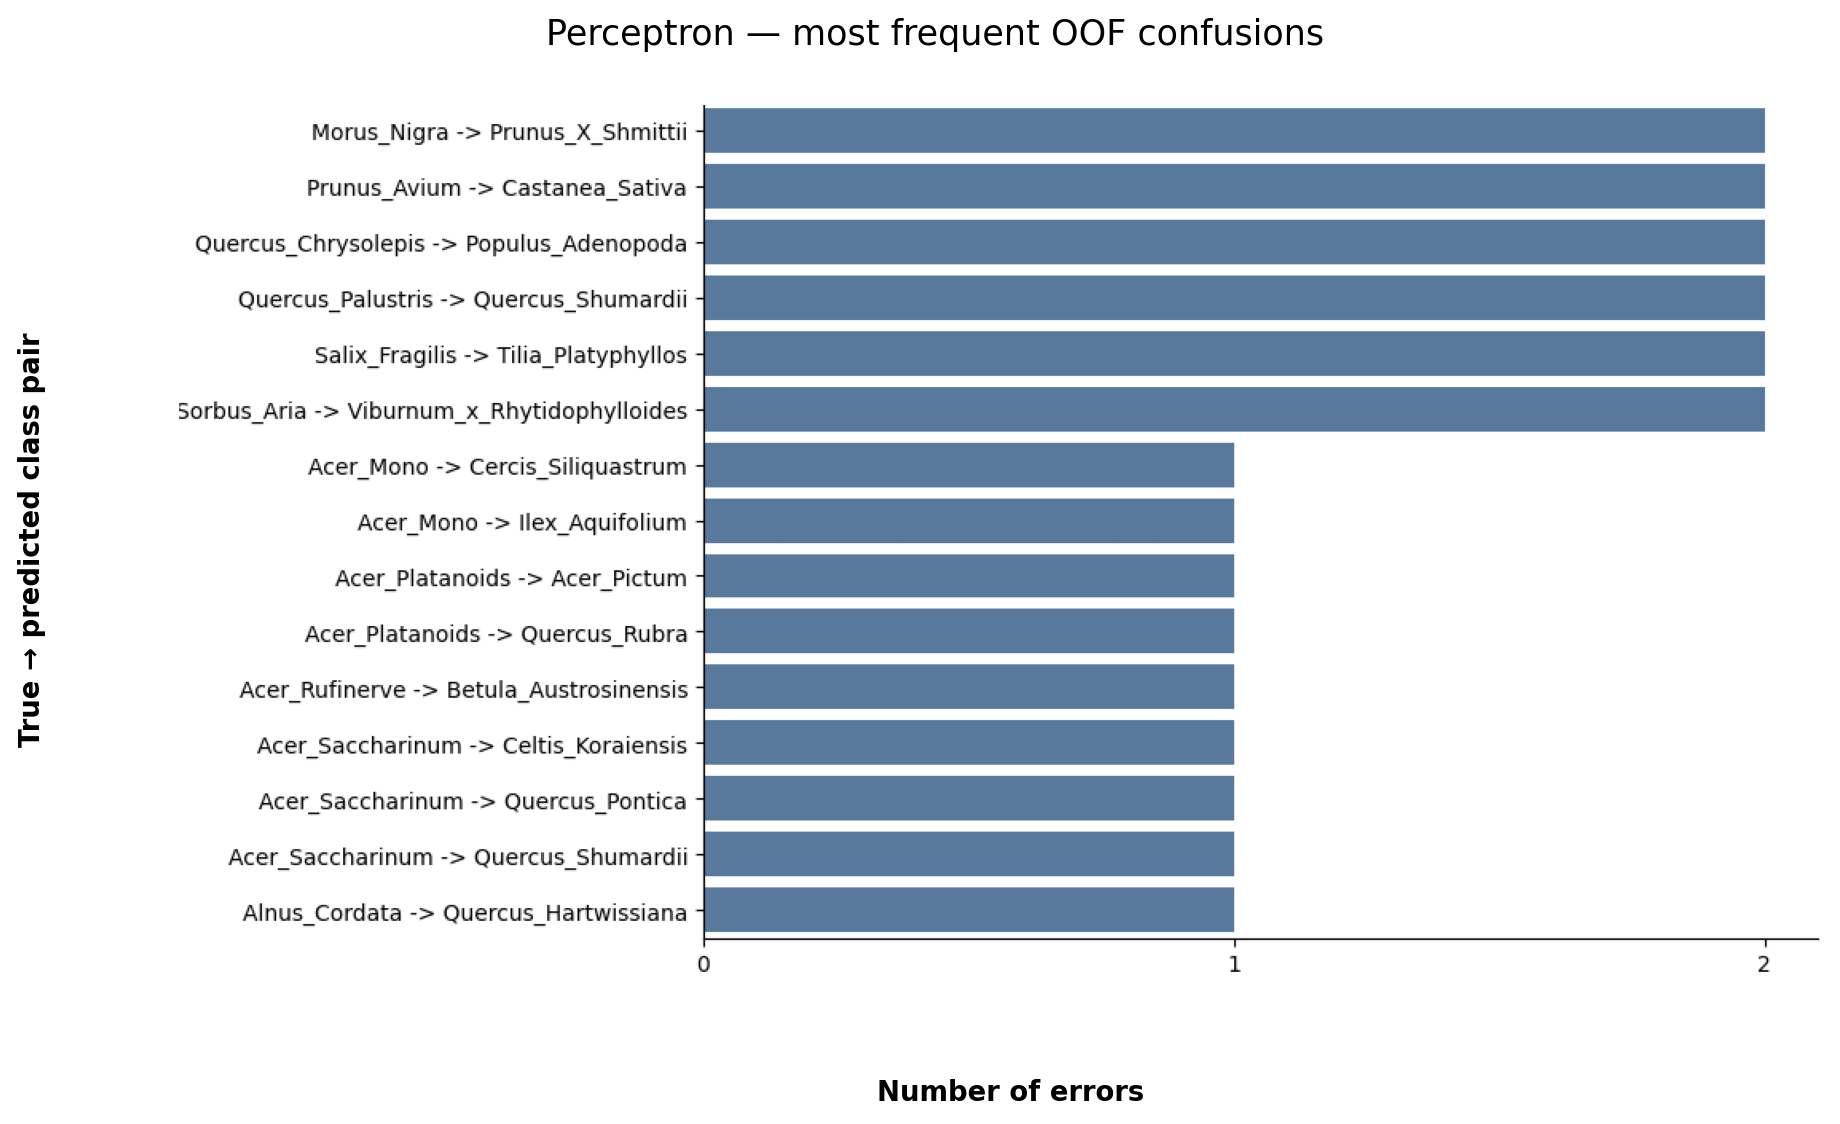
\includegraphics[width=\textwidth]{../figures/en/fig_perceptron_top12_confusions.png}
\caption{Leading confusions observed for the tuned perceptron. Their dispersion confirms that the model remains limited by its separation capacity.}
\end{figure}

\subsubsection{Secondary corroboration}
Secondary corroboration is available on the frozen split. The reference variant is \texttt{scaled\_only}, selected from the exploratory results on the development set. On the corroboration set, this reference achieves a \texttt{F1-macro} of \texttt{0.8815}, compared with \texttt{0.8694} for the \texttt{tuned} variant. The \texttt{tuned - reference} delta is therefore \texttt{-0.0121}.

\begin{table}[H]
\centering
\begin{tabular}{|l|r|r|l|}
\hline
\textbf{Variant} & \textbf{Corroboration F1} & \textbf{Corroboration accuracy} & \textbf{Role} \\
\hline
\texttt{default} & \texttt{0.8318} & \texttt{0.8586} & baseline \\
\texttt{scaled\_only} & \texttt{0.8815} & \texttt{0.8939} & reference \\
\texttt{scaled\_pca} & \texttt{0.8671} & \texttt{0.8838} & descriptive \\
\texttt{tuned} & \texttt{0.8694} & \texttt{0.8838} & tuned \\
\hline
\end{tabular}
\end{table}

For the perceptron, corroboration primarily confirms that the useful gain comes from standardization. Tuning provides no robust improvement for this inflexible family, which therefore remains chiefly an informative linear baseline.

\begin{figure}[H]
\centering
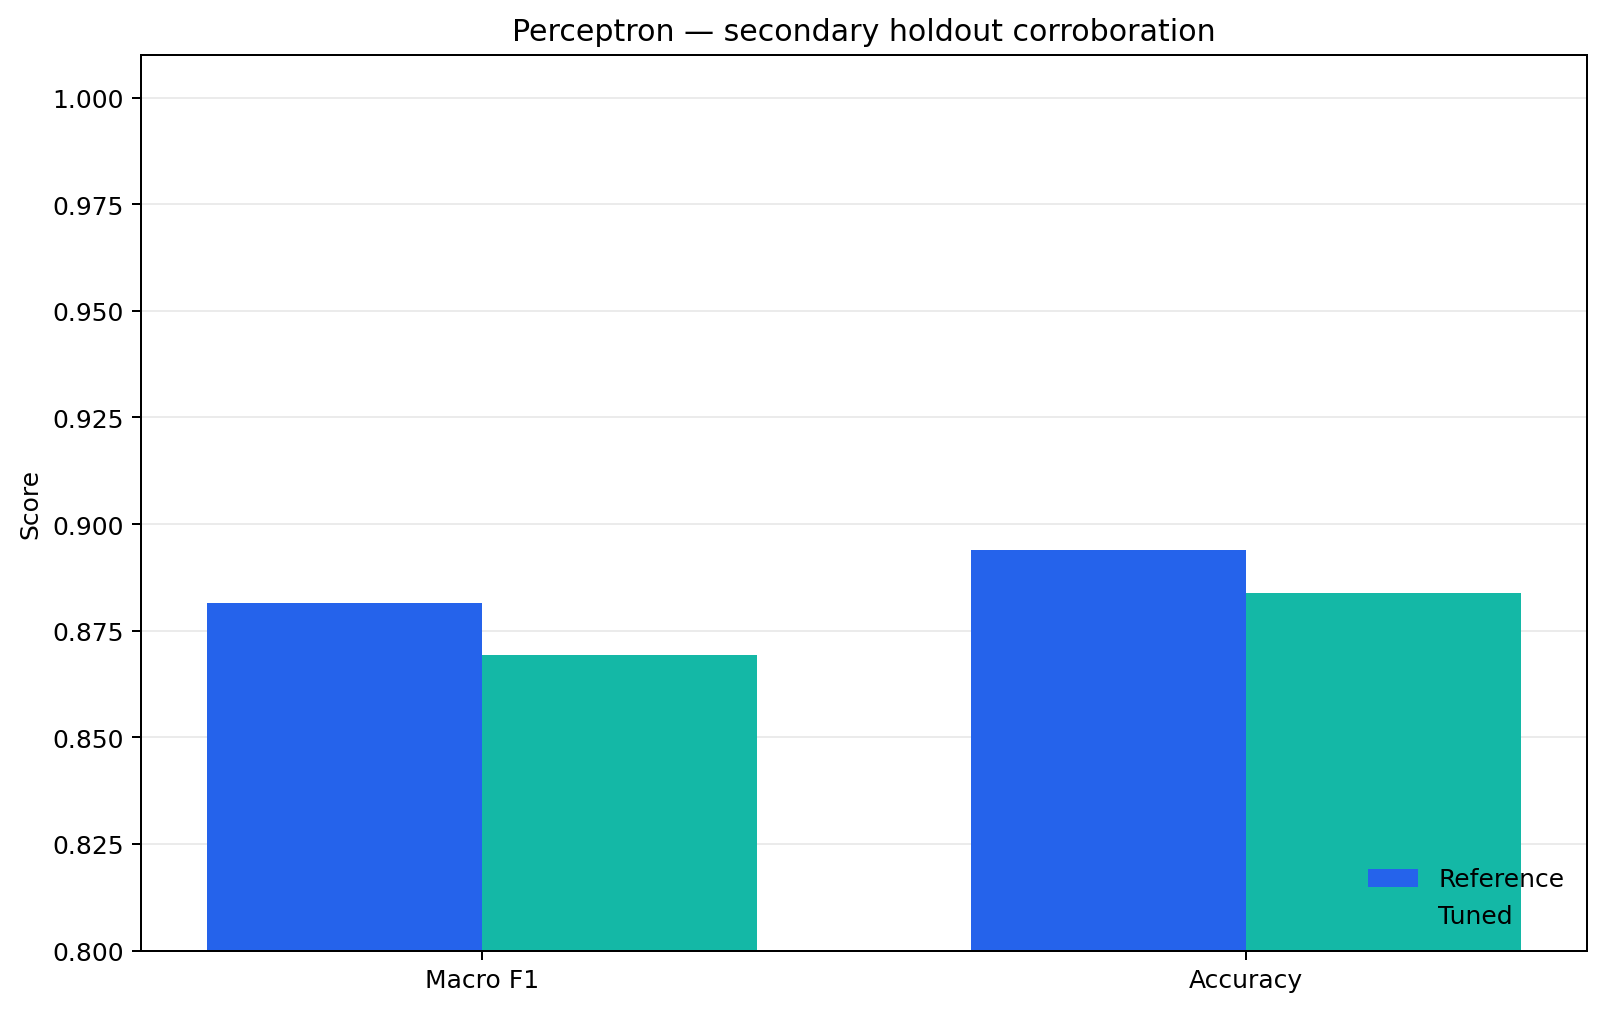
\includegraphics[width=\textwidth]{../figures/en/fig_perceptron_corroboration_holdout.png}
\caption{Secondary comparison between the reference and \texttt{tuned} perceptron variants on the corroboration set.}
\end{figure}

% --- LOGISTIC REGRESSION ---
\subsection{Logistic regression model}

\subsubsection{Role of the model}
Logistic regression is the project's probabilistic linear reference. It combines a simple decision structure, controlled regularization, and interpretable probabilities, making it a particularly strong anchor for assessing both predictive performance and the quality of probabilistic outputs.

\subsubsection{Exploration}
The exploratory results reveal a very strong dependence on scaling. Without preprocessing, logistic regression reaches only \texttt{0.2591} in \texttt{F1-macro} and \texttt{0.3106} in \texttt{accuracy}. With \texttt{StandardScaler}, it rises to \texttt{0.9798} in \texttt{F1-macro} and \texttt{0.9861} in \texttt{accuracy}. The \texttt{scaled\_pca} variant remains almost level with it (\texttt{0.9784} in \texttt{F1-macro}), with no robust gain over scaling alone.

\begin{table}[H]
\centering
\begin{tabular}{|l|l|r|r|r|r|}
\hline
\textbf{Variant} & \textbf{Protocol} & \textbf{Macro F1} & \textbf{Accuracy} & \textbf{F1 gap} & \textbf{Time (s)} \\
\hline
\texttt{default} & simple CV & \texttt{0.2591} & \texttt{0.3106} & \texttt{0.0899} & \texttt{1.69} \\
\texttt{scaled\_only} & simple CV & \texttt{0.9798} & \texttt{0.9861} & \texttt{0.0202} & \texttt{8.10} \\
\texttt{scaled\_pca} & simple CV & \texttt{0.9784} & \texttt{0.9848} & \texttt{0.0216} & \texttt{2.21} \\
\hline
\end{tabular}
\end{table}

This stage already establishes a strong result: on this dataset, a well-regularized linear model becomes extremely effective once supplied with correctly standardized variables. The family therefore immediately emerges as one of the leading candidates in the final ranking.

\begin{figure}[H]
\centering
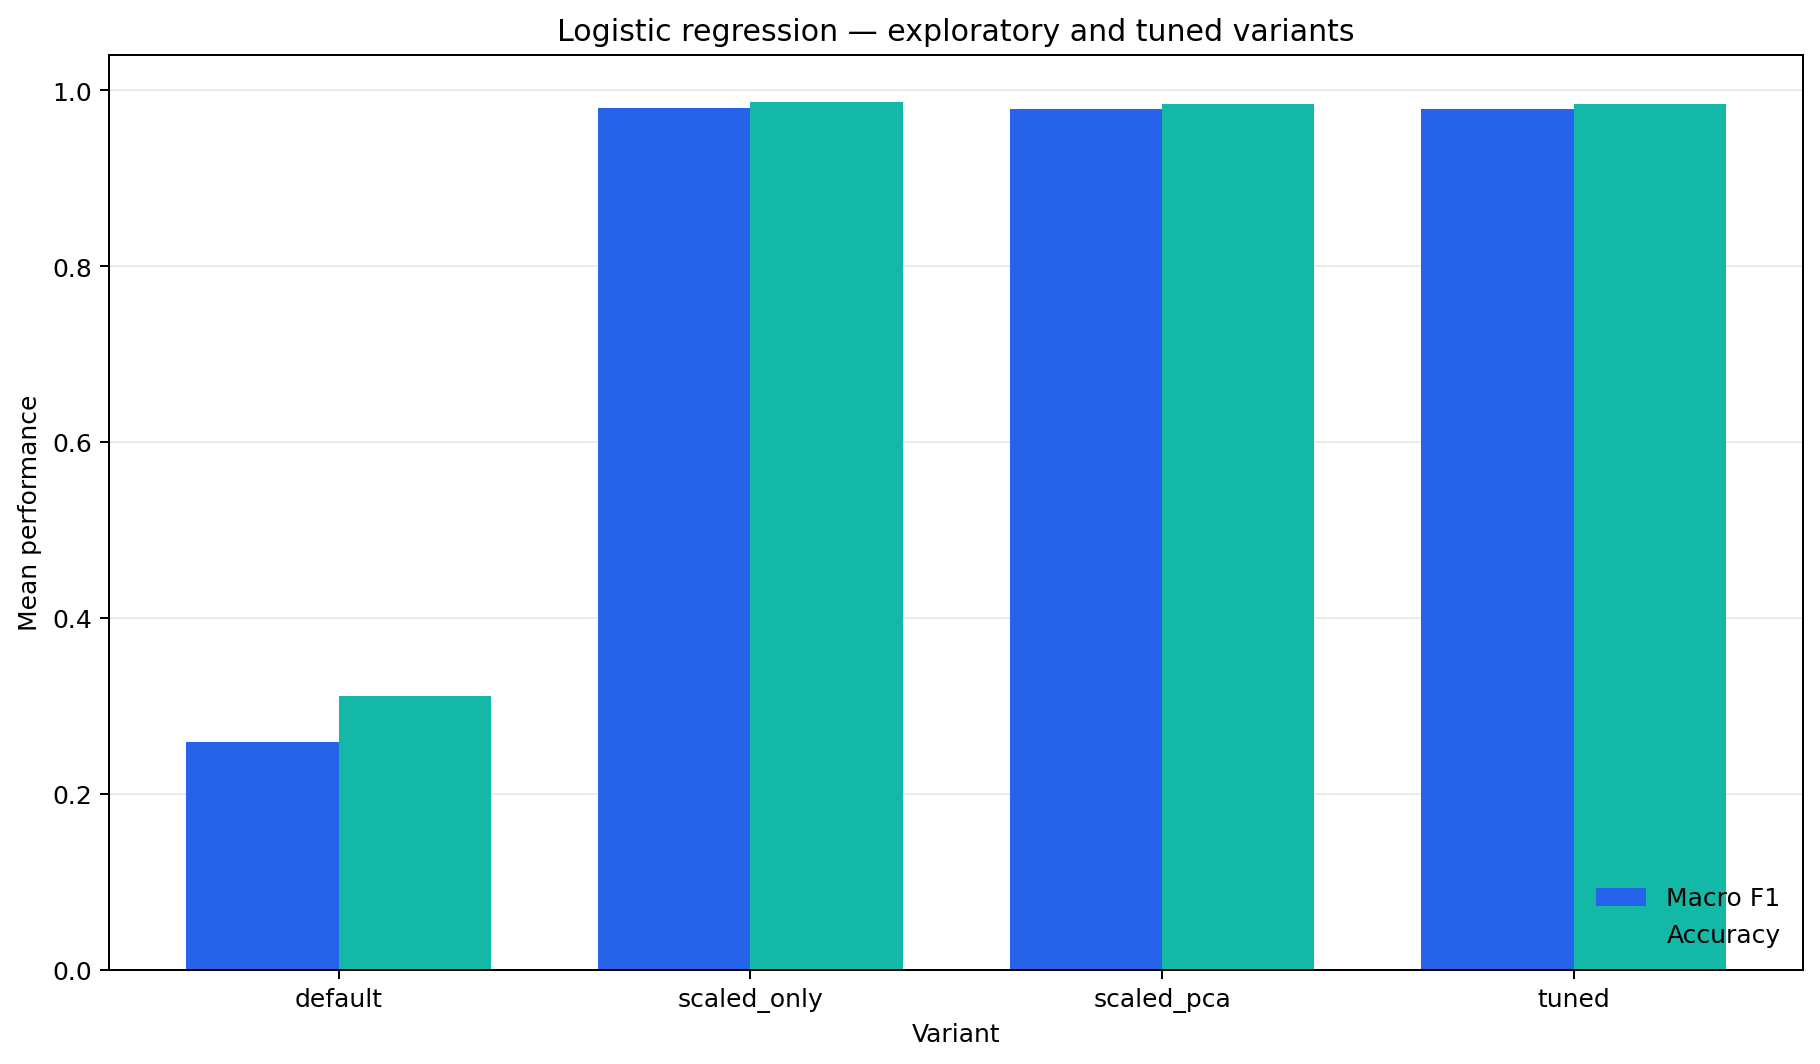
\includegraphics[width=\textwidth]{../figures/en/fig_lr_comparaison_variantes.png}
\caption{Exploratory comparison of logistic-regression variants. Scaling transforms a weak linear model into one of the study's best-performing classifiers.}
\end{figure}

\subsubsection{Confirmation}
Nested cross-validation fully confirms this interpretation. The \texttt{tuned} variant achieves a mean \texttt{F1-macro} of \texttt{0.9787} and mean \texttt{accuracy} of \texttt{0.9848}, with standard deviations of \texttt{0.0198} and \texttt{0.0146}. The confirmatory estimate is virtually identical to that of the best exploratory variant, indicating excellent signal stability.

\begin{table}[H]
\centering
\begin{tabular}{|l|r|}
\hline
\textbf{Confirmatory metric} & \textbf{Value} \\
\hline
Mean Macro F1 & \texttt{0.9787} \\
F1 standard deviation & \texttt{0.0198} \\
Mean accuracy & \texttt{0.9848} \\
Accuracy standard deviation & \texttt{0.0146} \\
Protocol & \texttt{nested CV} \\
Outer folds & \texttt{5} \\
Inner folds & \texttt{3} \\
Total time (s) & \texttt{77.05} \\
\hline
\end{tabular}
\end{table}

Logistic regression leads the confirmatory means and, together with the SVM, forms the report's top pair. Its strength does not come from complex tuning, but from the remarkable fit between linear regularization, standardization, and the structure of the problem.

\subsubsection{Descriptive diagnostics}
The diagnostics for this family help explain why it performs so well. The regularization path shows that performance stabilizes quickly within the useful range of \texttt{C}, suggesting that the data already determine a strong boundary once scaling is applied. The leading residual confusions are also very few relative to the observed performance level.

\begin{figure}[H]
\centering
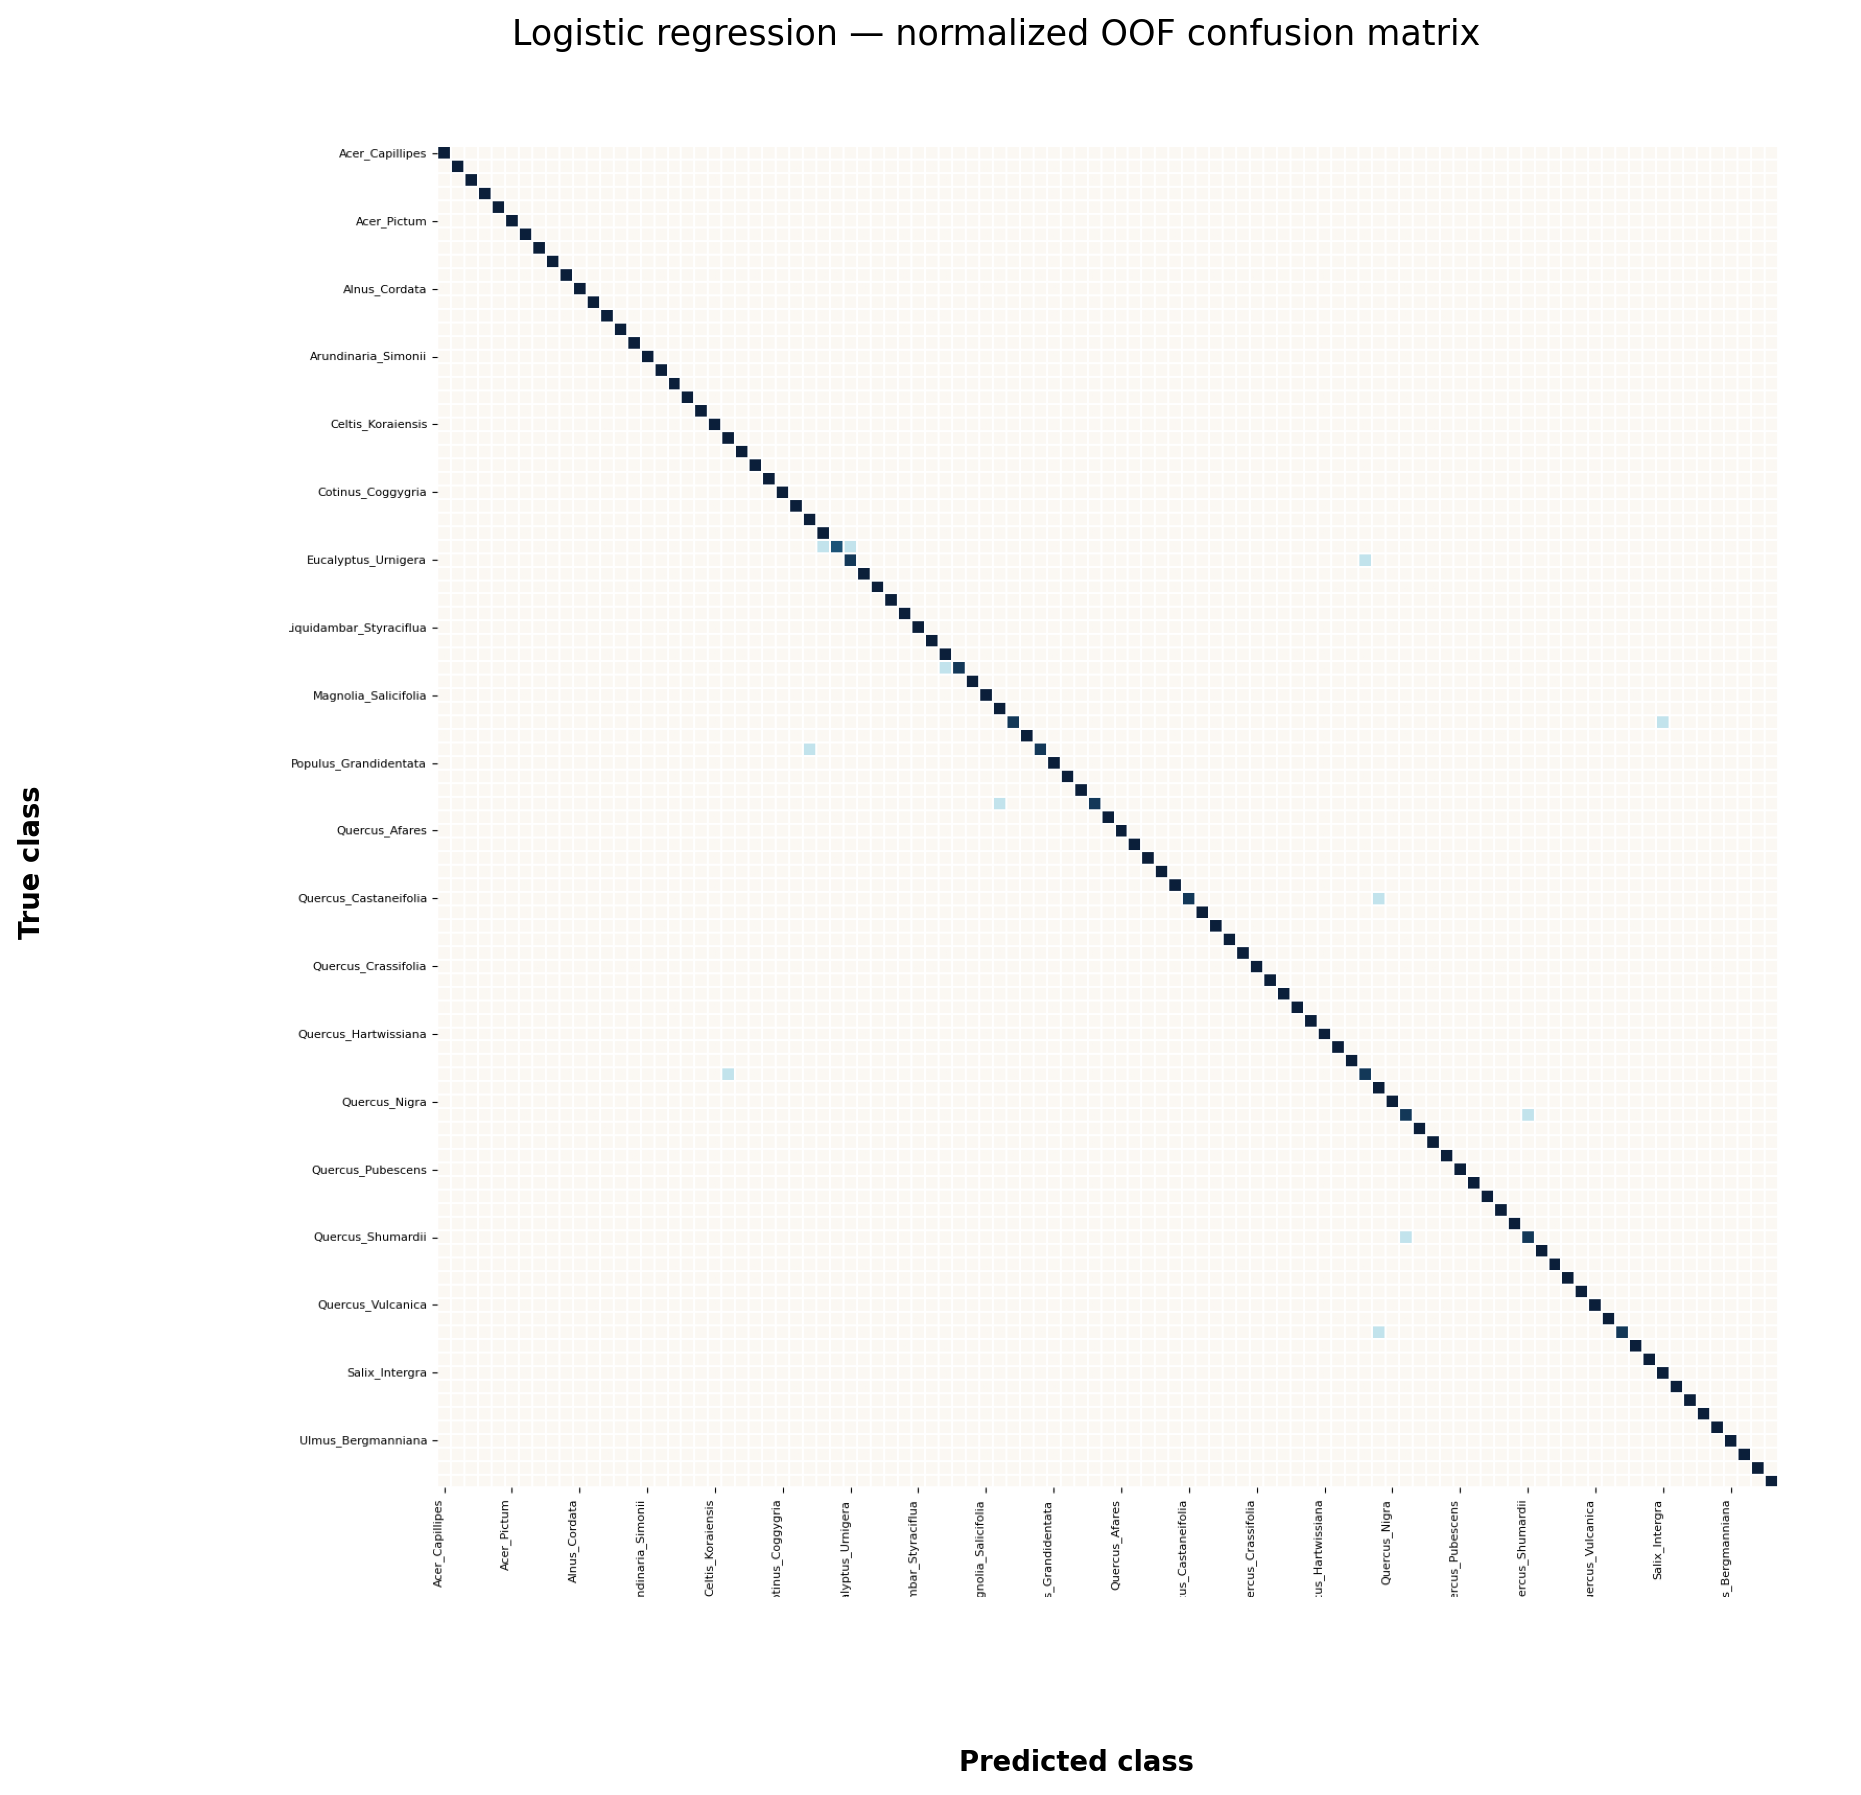
\includegraphics[width=\textwidth]{../figures/en/figA_confusion_lr_tuned.png}
\caption{Normalized confusion matrix from the out-of-fold predictions of the \texttt{tuned} variant. The near-diagonal structure confirms excellent separation among classes.}
\end{figure}

\begin{figure}[H]
\centering
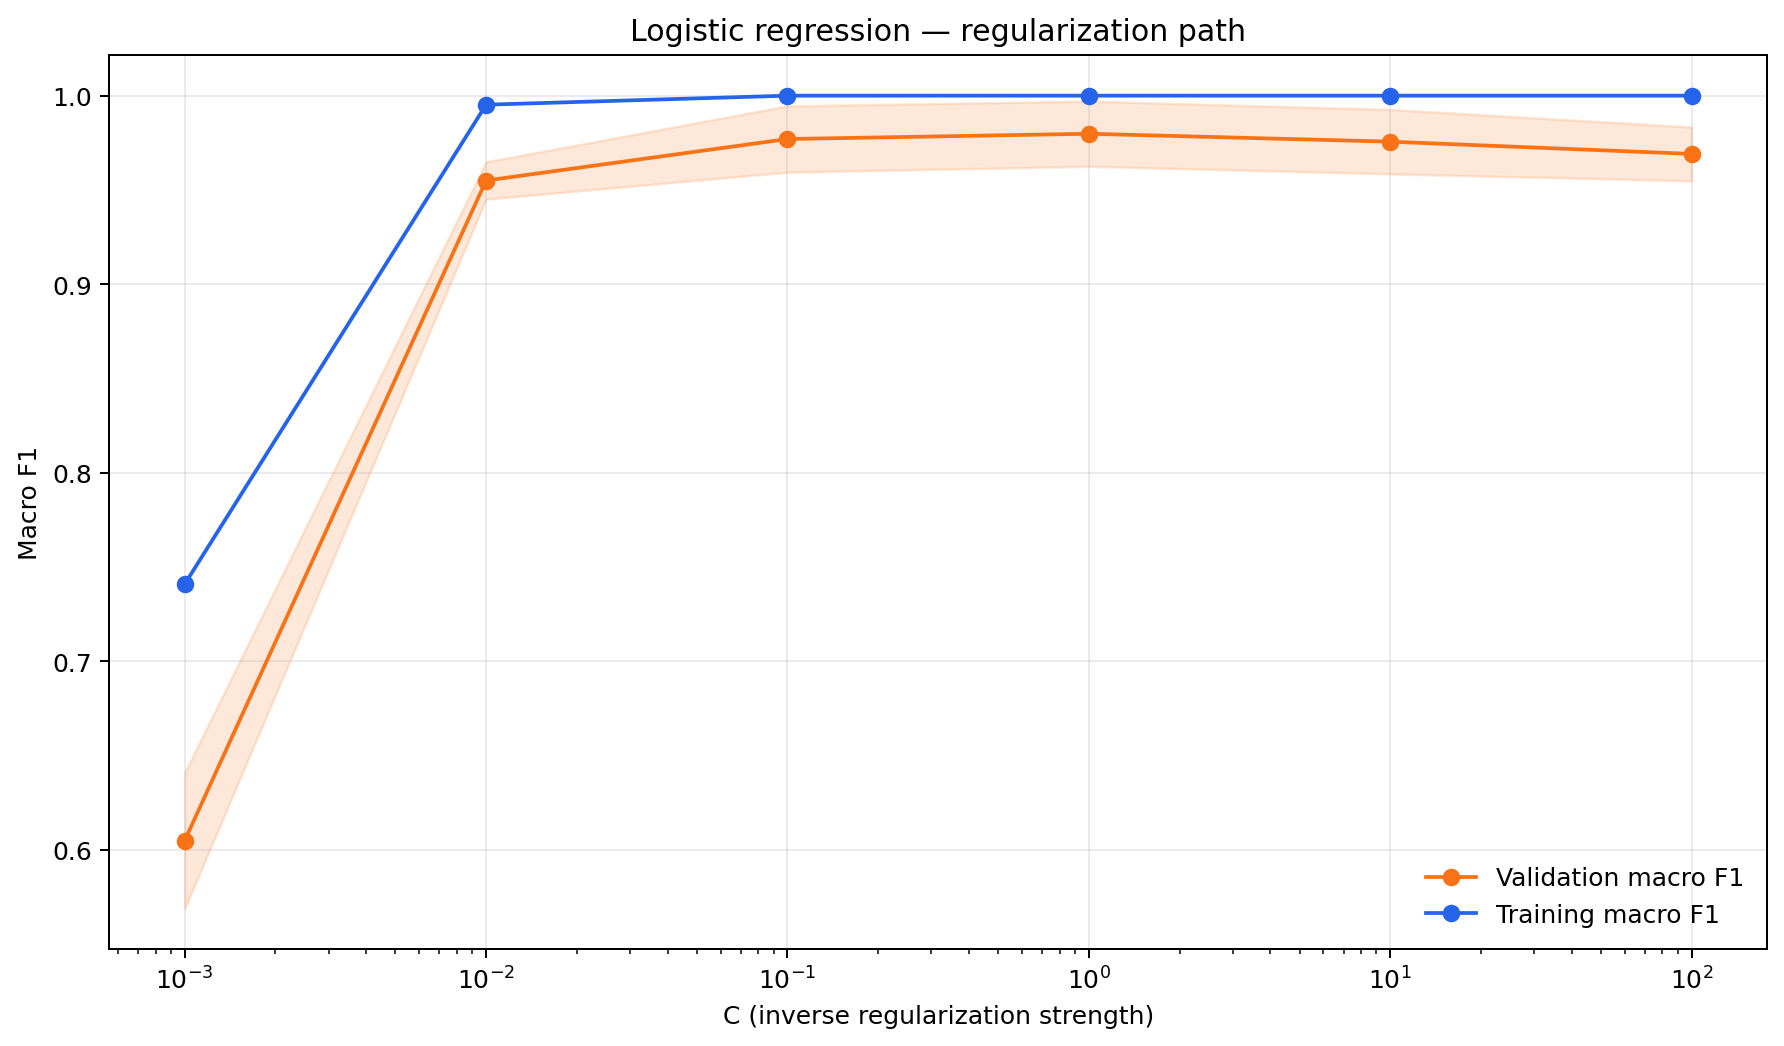
\includegraphics[width=\textwidth]{../figures/en/fig06_regularization_path.png}
\caption{Exploratory diagnostic of the tradeoff between regularization and performance. This figure supports model interpretation without replacing the confirmatory estimate.}
\end{figure}

\begin{figure}[H]
\centering
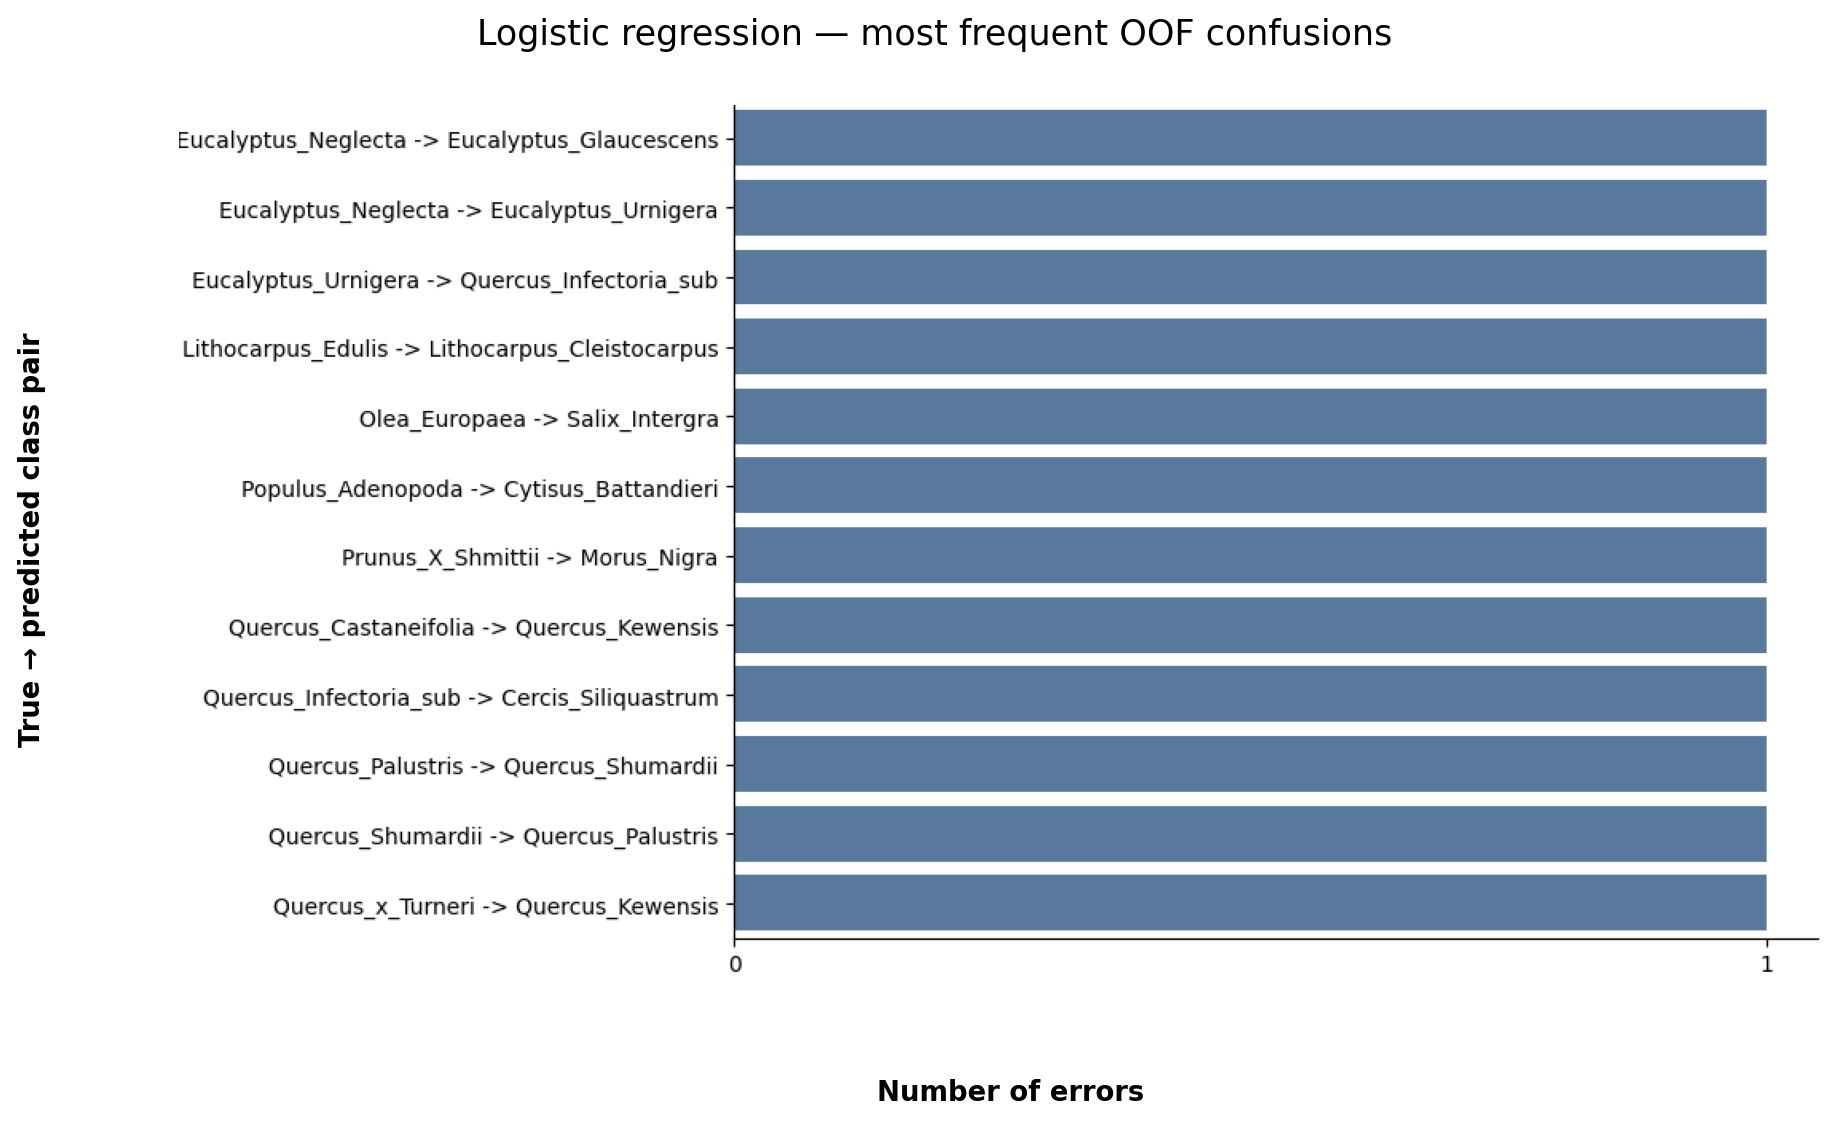
\includegraphics[width=\textwidth]{../figures/en/fig_lr_top12_confusions.png}
\caption{Leading residual confusions for logistic regression. Their small number is consistent with the observed confirmatory performance.}
\end{figure}

\subsubsection{Secondary corroboration}
Secondary corroboration fully supports the primary result. The \texttt{scaled\_only} reference, the \texttt{scaled\_pca} variant, and the \texttt{tuned} variant all achieve \texttt{0.9892} in \texttt{F1-macro} and \texttt{0.9899} in \texttt{accuracy} on the frozen split. The \texttt{tuned - reference} delta is therefore zero.

\begin{table}[H]
\centering
\begin{tabular}{|l|r|r|l|}
\hline
\textbf{Variant} & \textbf{Corroboration F1} & \textbf{Corroboration accuracy} & \textbf{Role} \\
\hline
\texttt{default} & \texttt{0.4800} & \texttt{0.5253} & baseline \\
\texttt{scaled\_only} & \texttt{0.9892} & \texttt{0.9899} & reference \\
\texttt{scaled\_pca} & \texttt{0.9892} & \texttt{0.9899} & descriptive \\
\texttt{tuned} & \texttt{0.9892} & \texttt{0.9899} & tuned \\
\hline
\end{tabular}
\end{table}

For logistic regression, corroboration extends a result already evident in the preceding analyses: after standardization, the family is both highly effective and remarkably stable. This combination, even more than tuning itself, makes it the report's practical reference.

\begin{figure}[H]
\centering
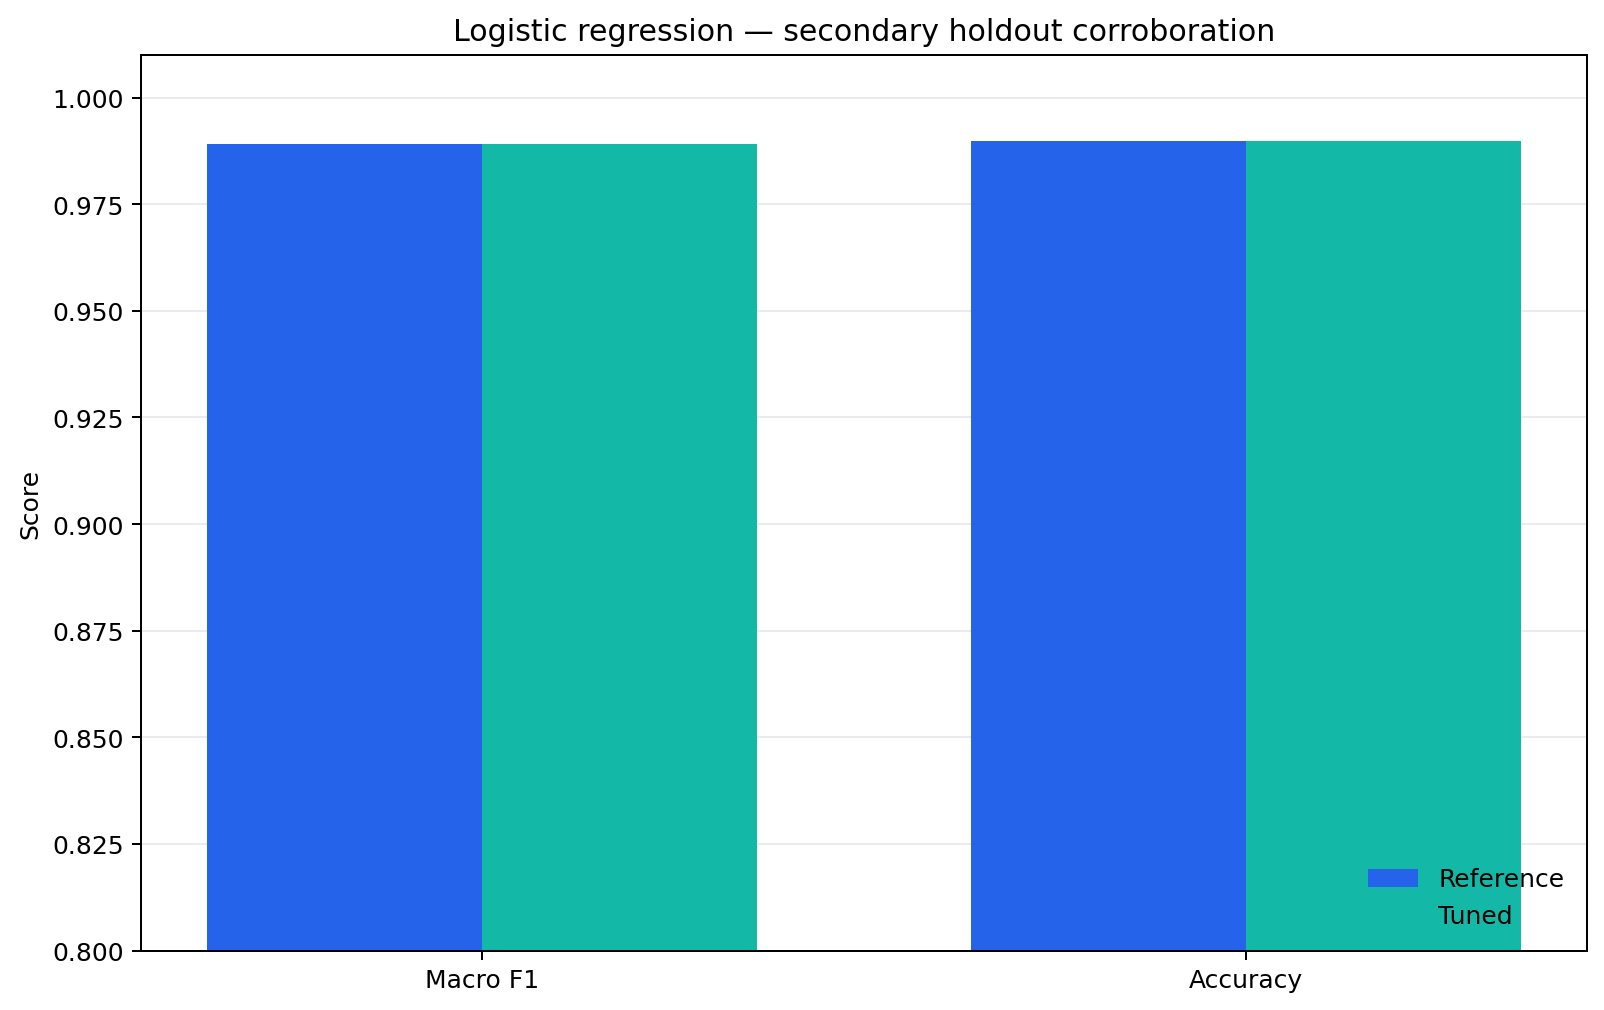
\includegraphics[width=\textwidth]{../figures/en/fig_lr_corroboration_holdout.png}
\caption{Secondary comparison between the reference and \texttt{tuned} logistic-regression variants on the corroboration set.}
\end{figure}

% --- SVM ---
\subsection{RBF SVM model}

\subsubsection{Role of the model}
The RBF-kernel SVM is the reference nonlinear margin-based method. Its purpose is to determine whether a more flexible boundary than that of the linear models can provide a tangible gain while remaining controlled on a moderately sized dataset.

\subsubsection{Exploration}
The SVM is already strong without preprocessing, with a \texttt{F1-macro} of \texttt{0.8389} and an \texttt{accuracy} of \texttt{0.8561}. Standardization nevertheless produces a clear change in scale: both \texttt{scaled\_only} and \texttt{scaled\_pca} reach \texttt{0.9712} in \texttt{F1-macro} and \texttt{0.9785} in \texttt{accuracy}. \texttt{PCA} therefore does not change the empirical interpretation, whereas scaling appears to be the decisive condition for using the RBF kernel effectively.

\begin{table}[H]
\centering
\begin{tabular}{|l|l|r|r|r|r|}
\hline
\textbf{Variant} & \textbf{Protocol} & \textbf{Macro F1} & \textbf{Accuracy} & \textbf{F1 gap} & \textbf{Time (s)} \\
\hline
\texttt{default} & simple CV & \texttt{0.8389} & \texttt{0.8561} & \texttt{0.1364} & \texttt{2.36} \\
\texttt{scaled\_only} & simple CV & \texttt{0.9712} & \texttt{0.9785} & \texttt{0.0266} & \texttt{2.45} \\
\texttt{scaled\_pca} & simple CV & \texttt{0.9712} & \texttt{0.9785} & \texttt{0.0266} & \texttt{2.50} \\
\hline
\end{tabular}
\end{table}

The SVM therefore joins the leading group during the exploratory stage. It combines very strong performance with a limited generalization gap, fully justifying its inclusion among the study's central models.

\begin{figure}[H]
\centering
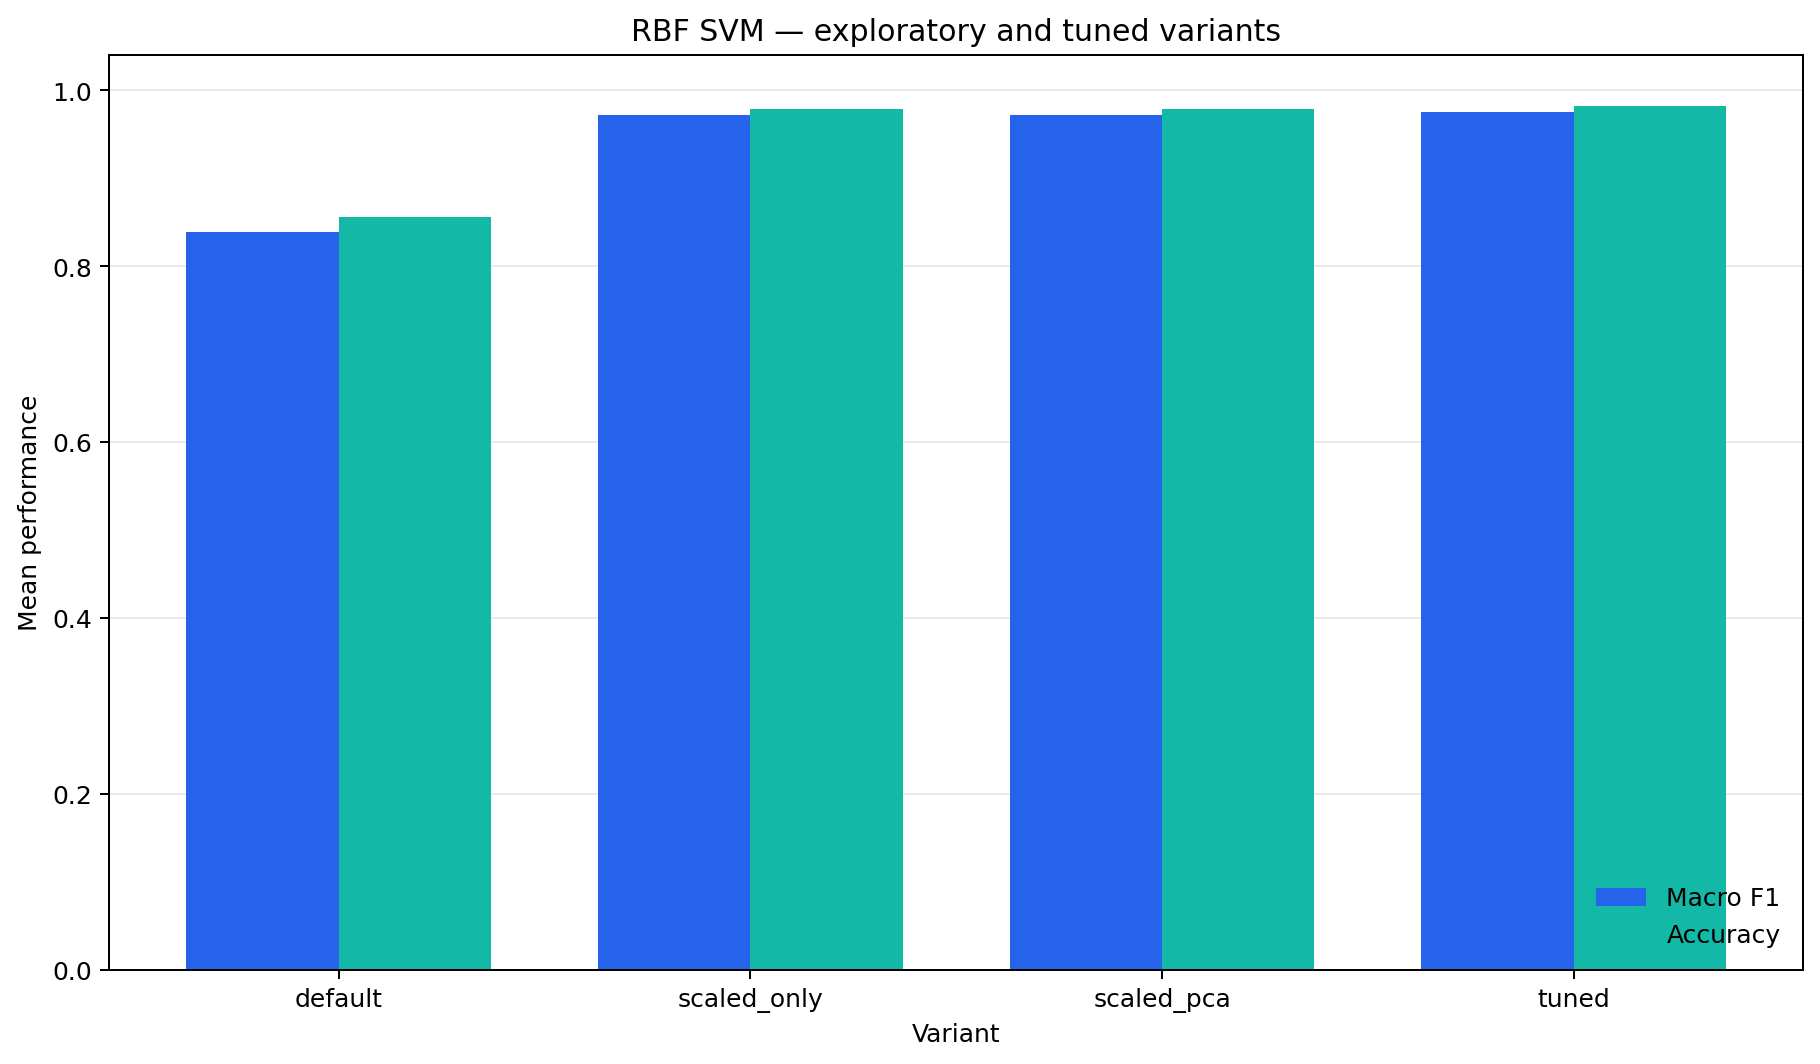
\includegraphics[width=\textwidth]{../figures/en/fig_svm_comparaison_variantes.png}
\caption{Exploratory comparison of SVM variants. The RBF kernel becomes fully competitive after feature standardization.}
\end{figure}

\subsubsection{Confirmation}
Nested cross-validation confirms this leading position. The \texttt{tuned} variant achieves a mean \texttt{F1-macro} of \texttt{0.9756} and mean \texttt{accuracy} of \texttt{0.9823}, with standard deviations of \texttt{0.0207} and \texttt{0.0151}. The confirmatory score is slightly higher than those of the best exploratory variants, suggesting that tuning is useful but moderate.

\begin{table}[H]
\centering
\begin{tabular}{|l|r|}
\hline
\textbf{Confirmatory metric} & \textbf{Value} \\
\hline
Mean Macro F1 & \texttt{0.9756} \\
F1 standard deviation & \texttt{0.0207} \\
Mean accuracy & \texttt{0.9823} \\
Accuracy standard deviation & \texttt{0.0151} \\
Protocol & \texttt{nested CV} \\
Outer folds & \texttt{5} \\
Inner folds & \texttt{3} \\
Total time (s) & \texttt{56.49} \\
\hline
\end{tabular}
\end{table}

The SVM also belongs to the leading confirmatory pair, with a mean very close to that of logistic regression. It therefore provides an excellent nonlinear alternative, at the cost of higher training time and lower structural interpretability.

\subsubsection{Descriptive diagnostics}
\begin{sloppypar}
The exploratory tuning table shows that the best performance is concentrated in a compact region of the hyperparameter space. Two findings dominate. Setting \texttt{gamma = 0.1} sharply degrades the scores. In addition, \texttt{PCA} provides no robust gain over the standardized pipeline without dimensionality reduction. The best exploratory setting is therefore \texttt{C = 10} with \texttt{gamma = scale}, without \texttt{PCA}.
\end{sloppypar}

\begin{table}[H]
\centering
\begin{tabular}{|l|r|r|r|}
\hline
\textbf{C / gamma} & \textbf{scale} & \textbf{0.01} & \textbf{0.1} \\
\hline
\texttt{1} & \texttt{0.9697} & \texttt{0.9693} & \texttt{0.2539} \\
\texttt{10} & \texttt{0.9700} & \texttt{0.9679} & \texttt{0.2885} \\
\hline
\end{tabular}
\caption{Exploratory SVM tuning without PCA (mean CV \texttt{F1-macro})}
\end{table}

\begin{table}[H]
\centering
\begin{tabular}{|l|r|r|r|}
\hline
\textbf{C / gamma} & \textbf{scale} & \textbf{0.01} & \textbf{0.1} \\
\hline
\texttt{1} & \texttt{0.9697} & \texttt{0.9679} & \texttt{0.2917} \\
\texttt{10} & \texttt{0.9688} & \texttt{0.9654} & \texttt{0.3402} \\
\hline
\end{tabular}
\caption{Exploratory SVM tuning with PCA (mean CV \texttt{F1-macro})}
\end{table}

Residual confusions remain rare and localized, which is consistent with the quality of the confirmatory score.

\begin{figure}[H]
\centering
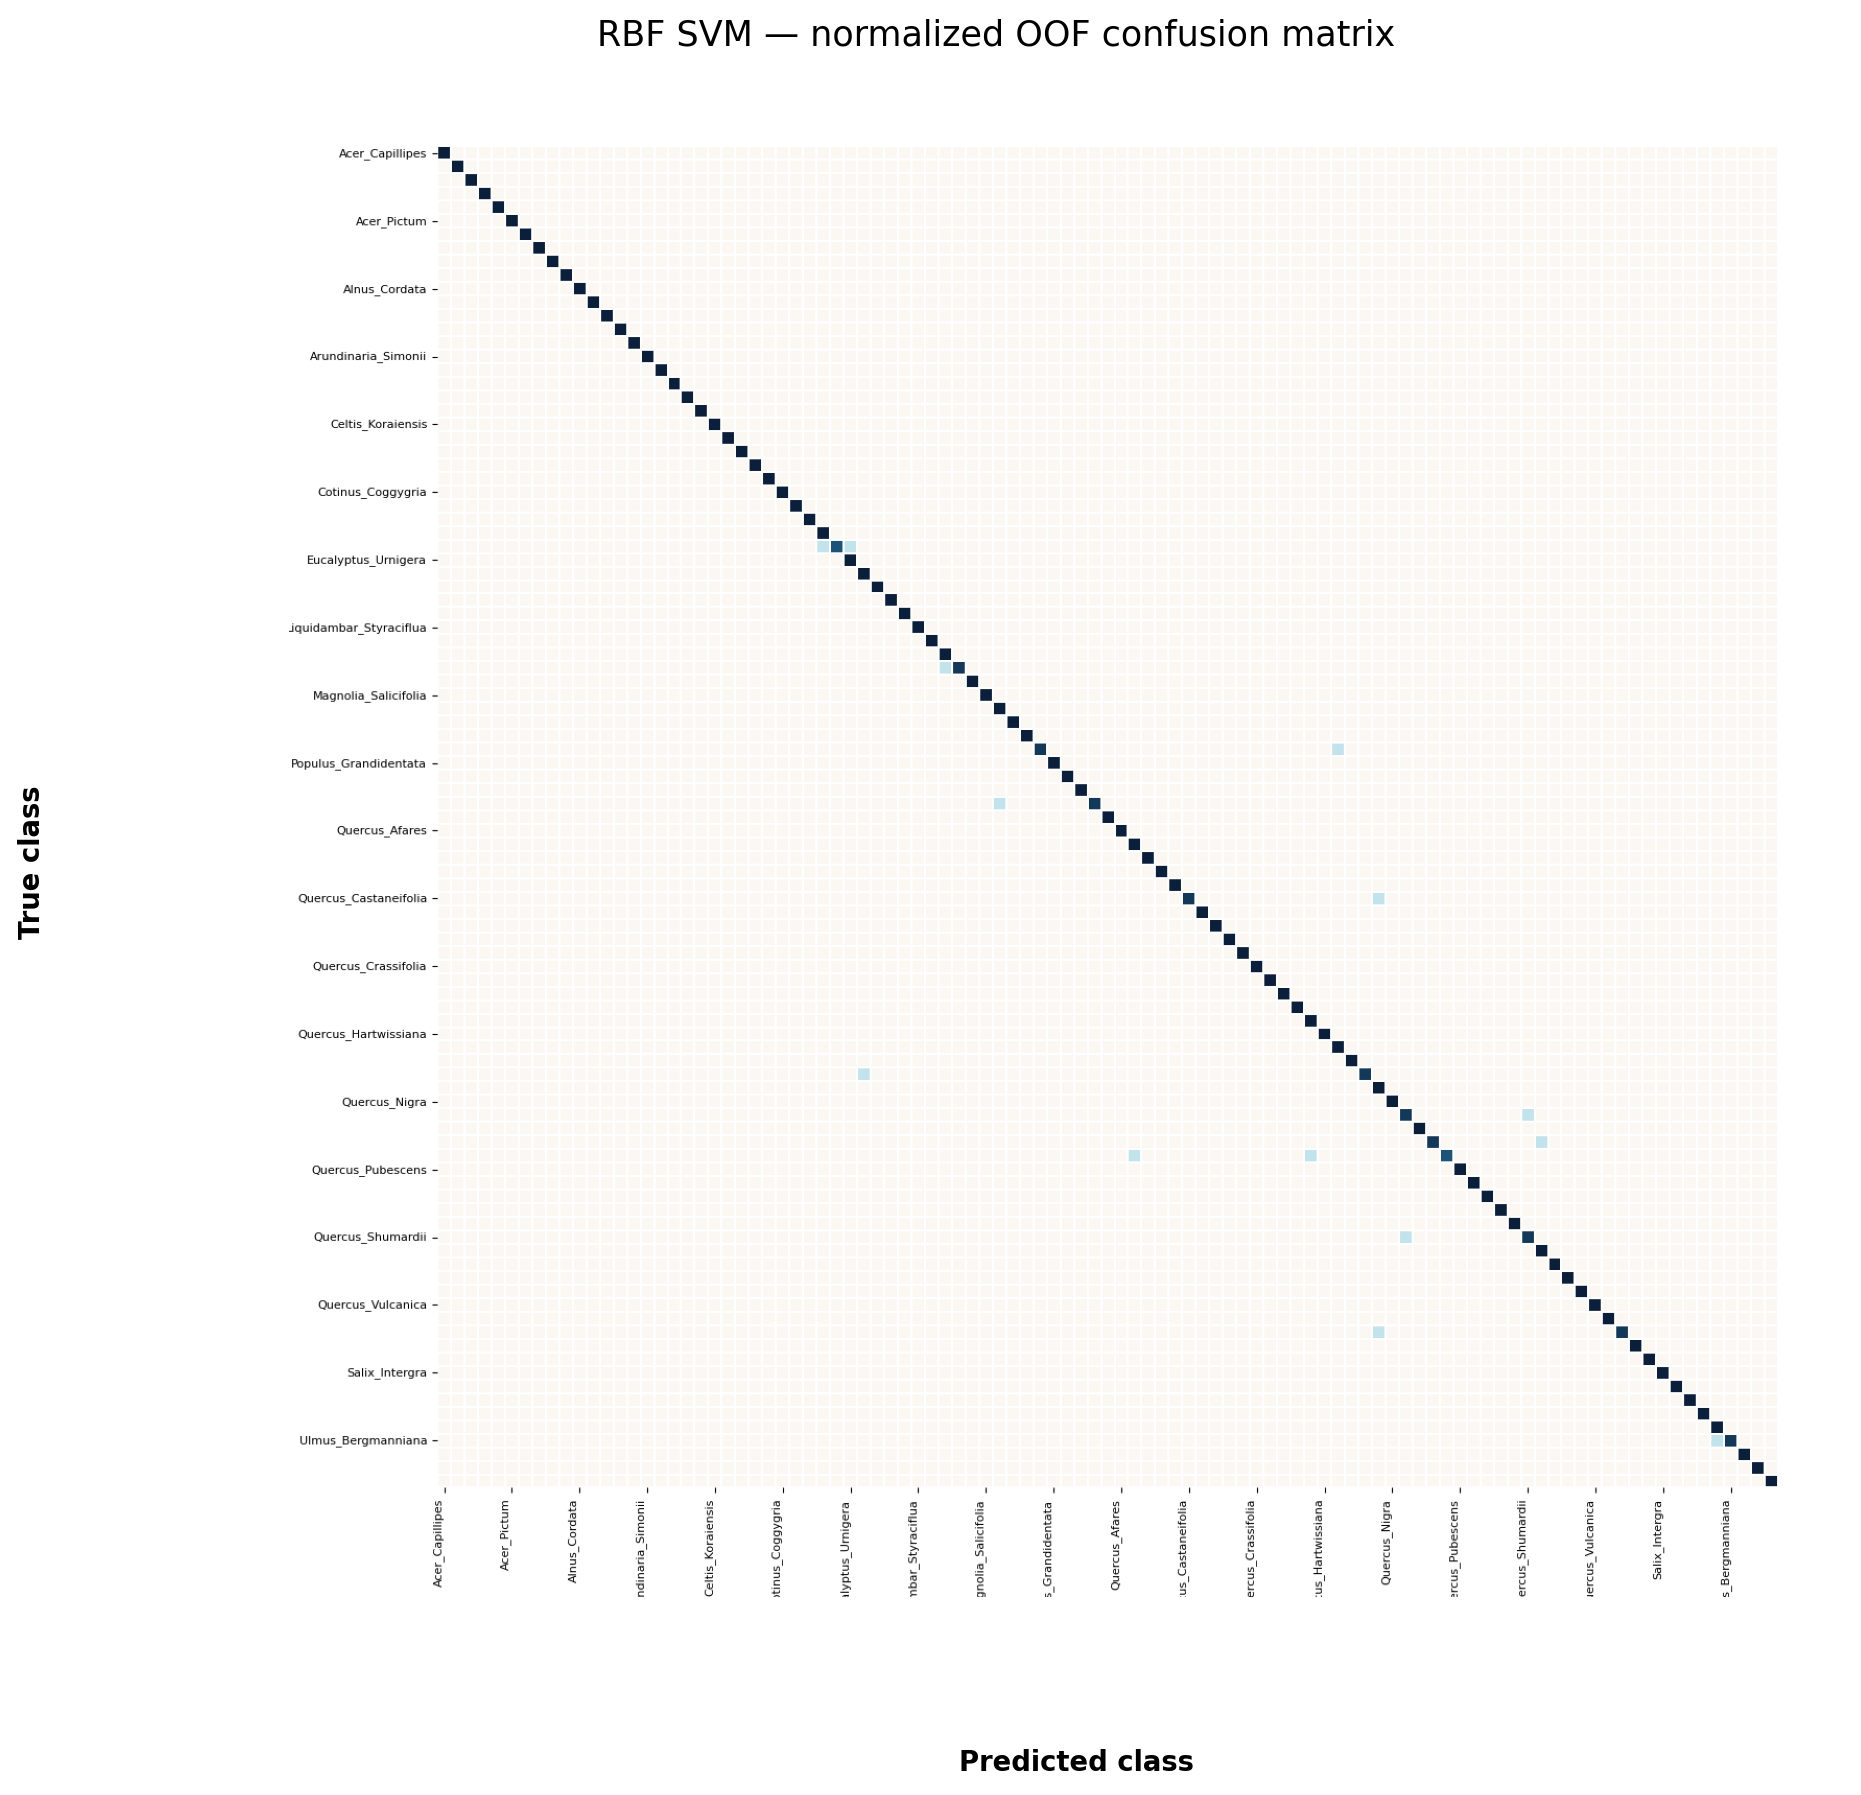
\includegraphics[width=\textwidth]{../figures/en/figA_confusion_svm_tuned.png}
\caption{Normalized confusion matrix from the out-of-fold predictions of the \texttt{tuned} variant. Residual errors are few and concentrated.}
\end{figure}

\begin{figure}[H]
\centering
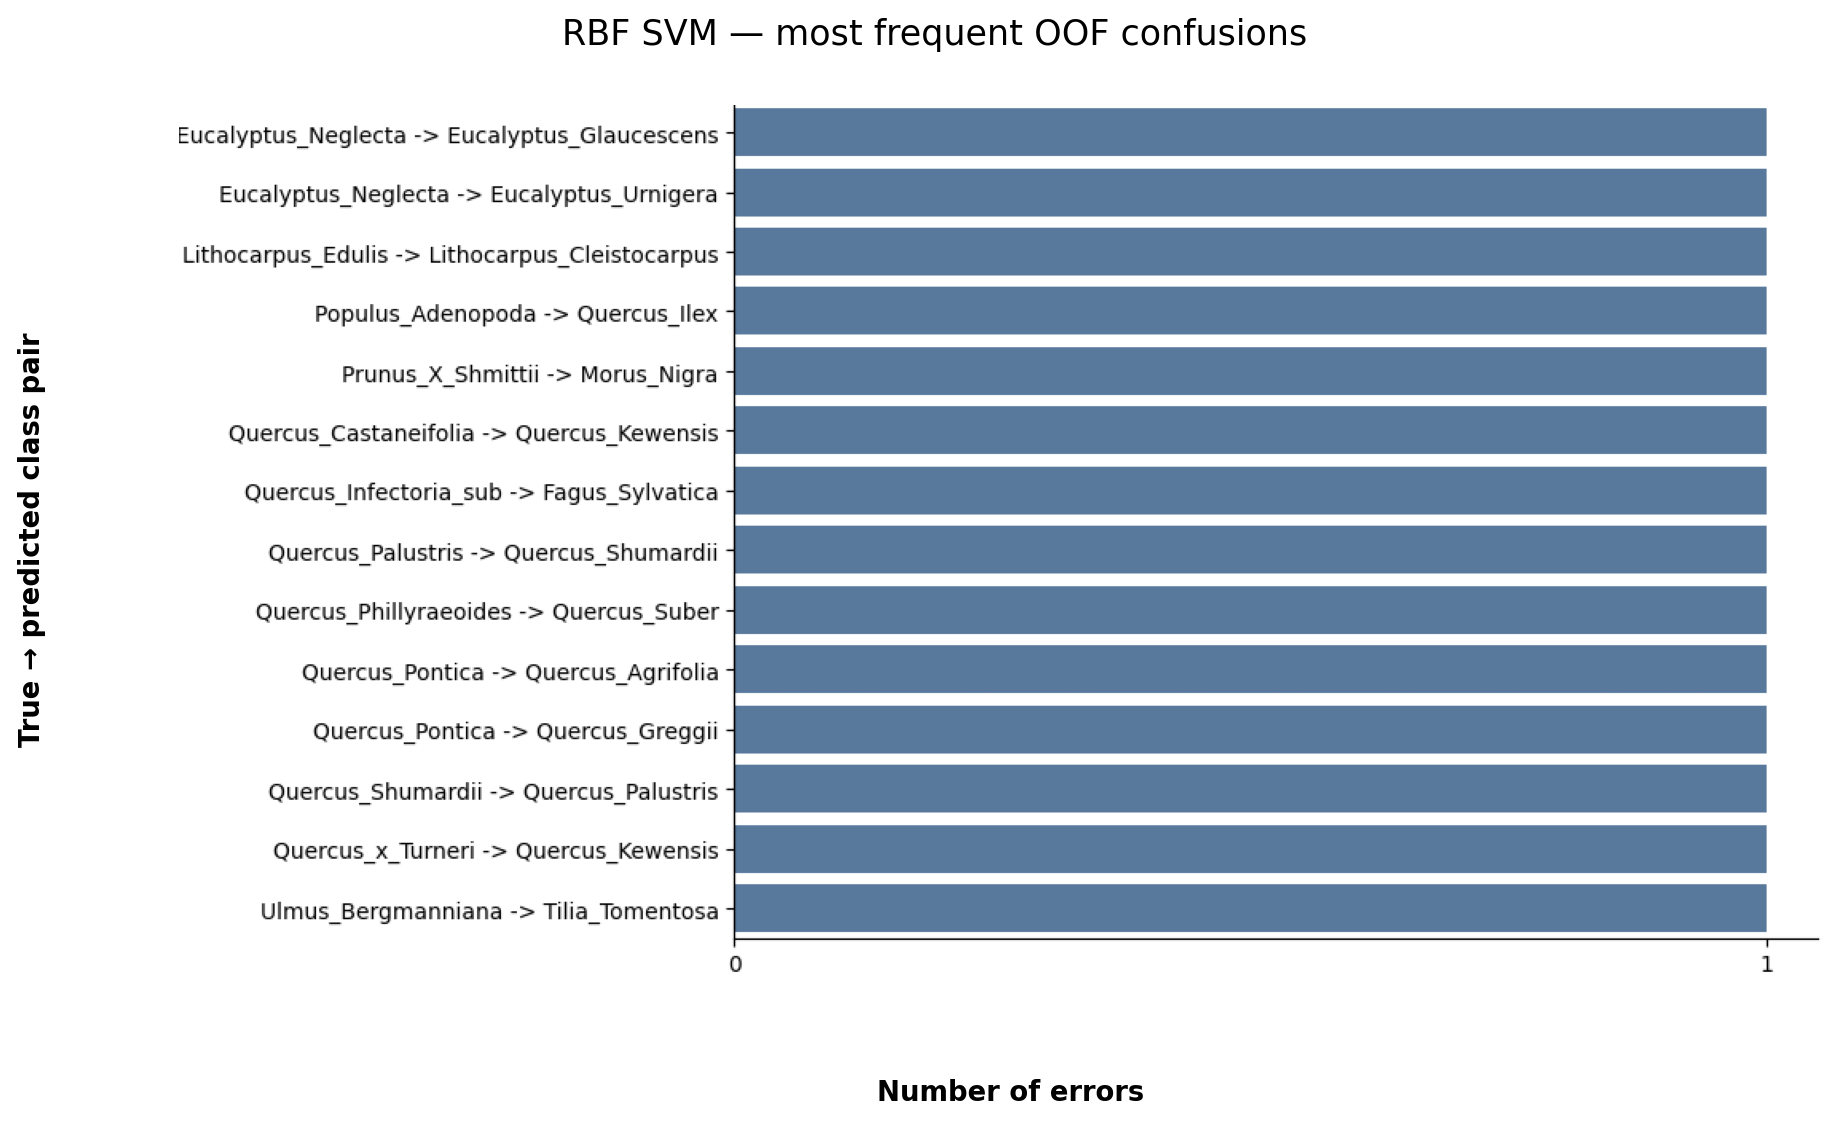
\includegraphics[width=\textwidth]{../figures/en/fig_svm_top12_confusions.png}
\caption{Leading confusions for the tuned SVM. Their limited number indicates that errors are concentrated among a few structurally difficult cases.}
\end{figure}

\subsubsection{Secondary corroboration}
Secondary corroboration is consistent with the confirmatory analysis and provides an even more favorable signal for tuning. The \texttt{scaled\_only} reference achieves \texttt{0.9838} in \texttt{F1-macro} and \texttt{0.9848} in \texttt{accuracy}, while the \texttt{tuned} variant reaches \texttt{0.9946} and \texttt{0.9949}. The \texttt{tuned - reference} delta is therefore \texttt{+0.0108}.

\begin{table}[H]
\centering
\begin{tabular}{|l|r|r|l|}
\hline
\textbf{Variant} & \textbf{Corroboration F1} & \textbf{Corroboration accuracy} & \textbf{Role} \\
\hline
\texttt{default} & \texttt{0.9242} & \texttt{0.9343} & baseline \\
\texttt{scaled\_only} & \texttt{0.9838} & \texttt{0.9848} & reference \\
\texttt{scaled\_pca} & \texttt{0.9838} & \texttt{0.9848} & descriptive \\
\texttt{tuned} & \texttt{0.9946} & \texttt{0.9949} & tuned \\
\hline
\end{tabular}
\end{table}

For the SVM, corroboration retains clear practical value: tuning remains beneficial on the frozen split. The family therefore emerges as one of the report's most compelling solutions, very close to logistic regression in performance but more dependent on careful hyperparameter selection.

\begin{figure}[H]
\centering
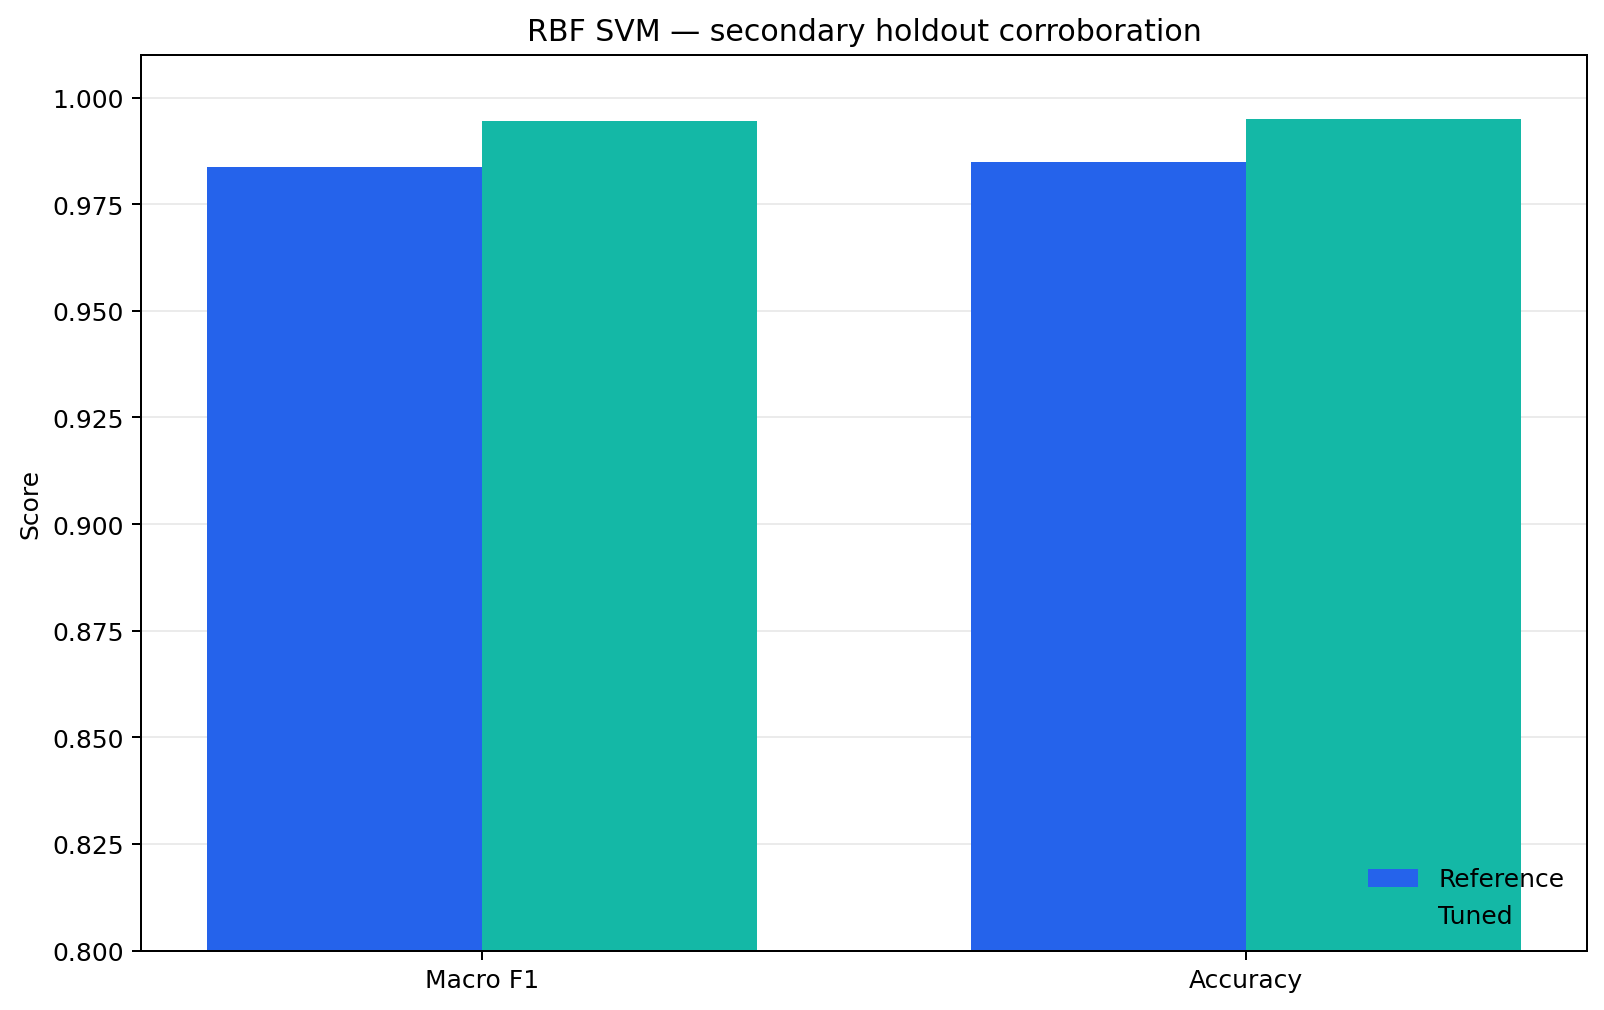
\includegraphics[width=\textwidth]{../figures/en/fig_svm_corroboration_holdout.png}
\caption{Secondary comparison between the reference and \texttt{tuned} SVM variants on the corroboration set.}
\end{figure}

% --- RANDOM FOREST ---
\subsection{Random forest model}

\subsubsection{Role of the model}
The random forest represents the study's tree-ensemble family. It is particularly relevant here because it can capture nonlinear interactions without requiring feature scaling and because it stabilizes the splits that a single decision tree struggles to generalize.

\subsubsection{Exploration}
The exploratory evidence is highly favorable for this family. The \texttt{default} variant achieves \texttt{0.9764} in \texttt{F1-macro} and \texttt{0.9785} in \texttt{accuracy}, with a contained generalization gap (\texttt{0.0236}). The \texttt{restricted\_depth} variant, added as a complexity control, falls to \texttt{0.9345} in \texttt{F1-macro} and \texttt{0.9445} in \texttt{accuracy}. Restricting depth therefore slightly reduces computation time but markedly degrades performance.

\begin{table}[H]
\centering
\begin{tabular}{|l|l|r|r|r|r|}
\hline
\textbf{Variant} & \textbf{Protocol} & \textbf{Macro F1} & \textbf{Accuracy} & \textbf{F1 gap} & \textbf{Time (s)} \\
\hline
\texttt{default} & simple CV & \texttt{0.9764} & \texttt{0.9785} & \texttt{0.0236} & \texttt{9.16} \\
\texttt{restricted\_depth} & simple CV & \texttt{0.9345} & \texttt{0.9445} & \texttt{0.0651} & \texttt{5.42} \\
\hline
\end{tabular}
\end{table}

Even at this stage, the random forest ranks among the project's best models. Its main strength is achieving this level without sophisticated preprocessing, making it a robust and straightforward option for already informative tabular variables.

\begin{figure}[H]
\centering
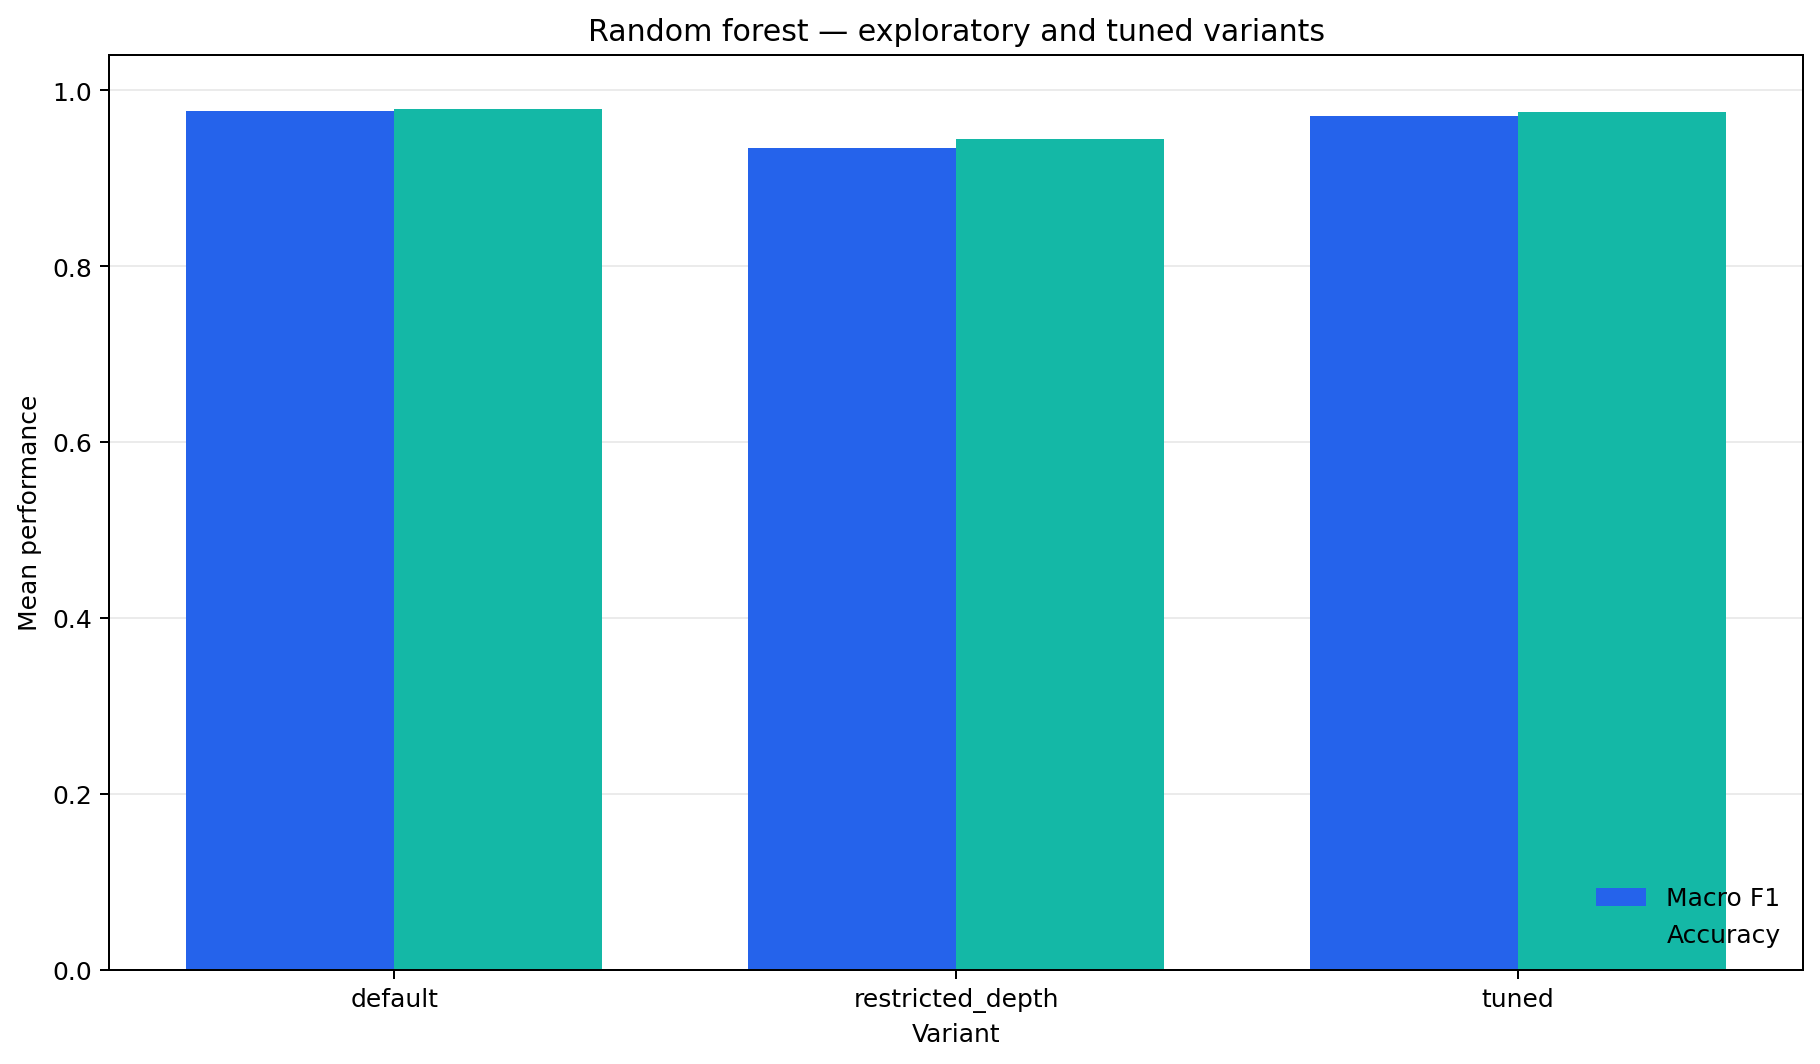
\includegraphics[width=\textwidth]{../figures/en/fig_rf_comparaison_variantes.png}
\caption{Exploratory comparison of random-forest variants. The default version already performs extremely well, and restricting depth proves too costly in performance.}
\end{figure}

\subsubsection{Confirmation}
Nested cross-validation yields a mean \texttt{F1-macro} of \texttt{0.9702} and mean \texttt{accuracy} of \texttt{0.9747}, with standard deviations of \texttt{0.0140} and \texttt{0.0089}. The confirmatory score remains slightly below that of the best exploratory variant, as expected when the estimate corrects for selection optimism.

\begin{table}[H]
\centering
\begin{tabular}{|l|r|}
\hline
\textbf{Confirmatory metric} & \textbf{Value} \\
\hline
Mean Macro F1 & \texttt{0.9702} \\
F1 standard deviation & \texttt{0.0140} \\
Mean accuracy & \texttt{0.9747} \\
Accuracy standard deviation & \texttt{0.0089} \\
Protocol & \texttt{nested CV} \\
Outer folds & \texttt{5} \\
Inner folds & \texttt{3} \\
Total time (s) & \texttt{250.11} \\
\hline
\end{tabular}
\end{table}

The random forest thus remains among the top three. It ranks slightly behind logistic regression and the SVM, but is still highly competitive and remarkably stable. Its main cost is a longer training time than the linear models.

\subsubsection{Descriptive diagnostics}
The \texttt{OOB} curve shows that marginal gains stabilize quickly as the number of trees increases. This pattern is fully consistent with the strong performance of the \texttt{default} variant and with tuning that is progressive rather than disruptive. The confusion figures further confirm that residual errors remain rare and structured.

\begin{figure}[H]
\centering
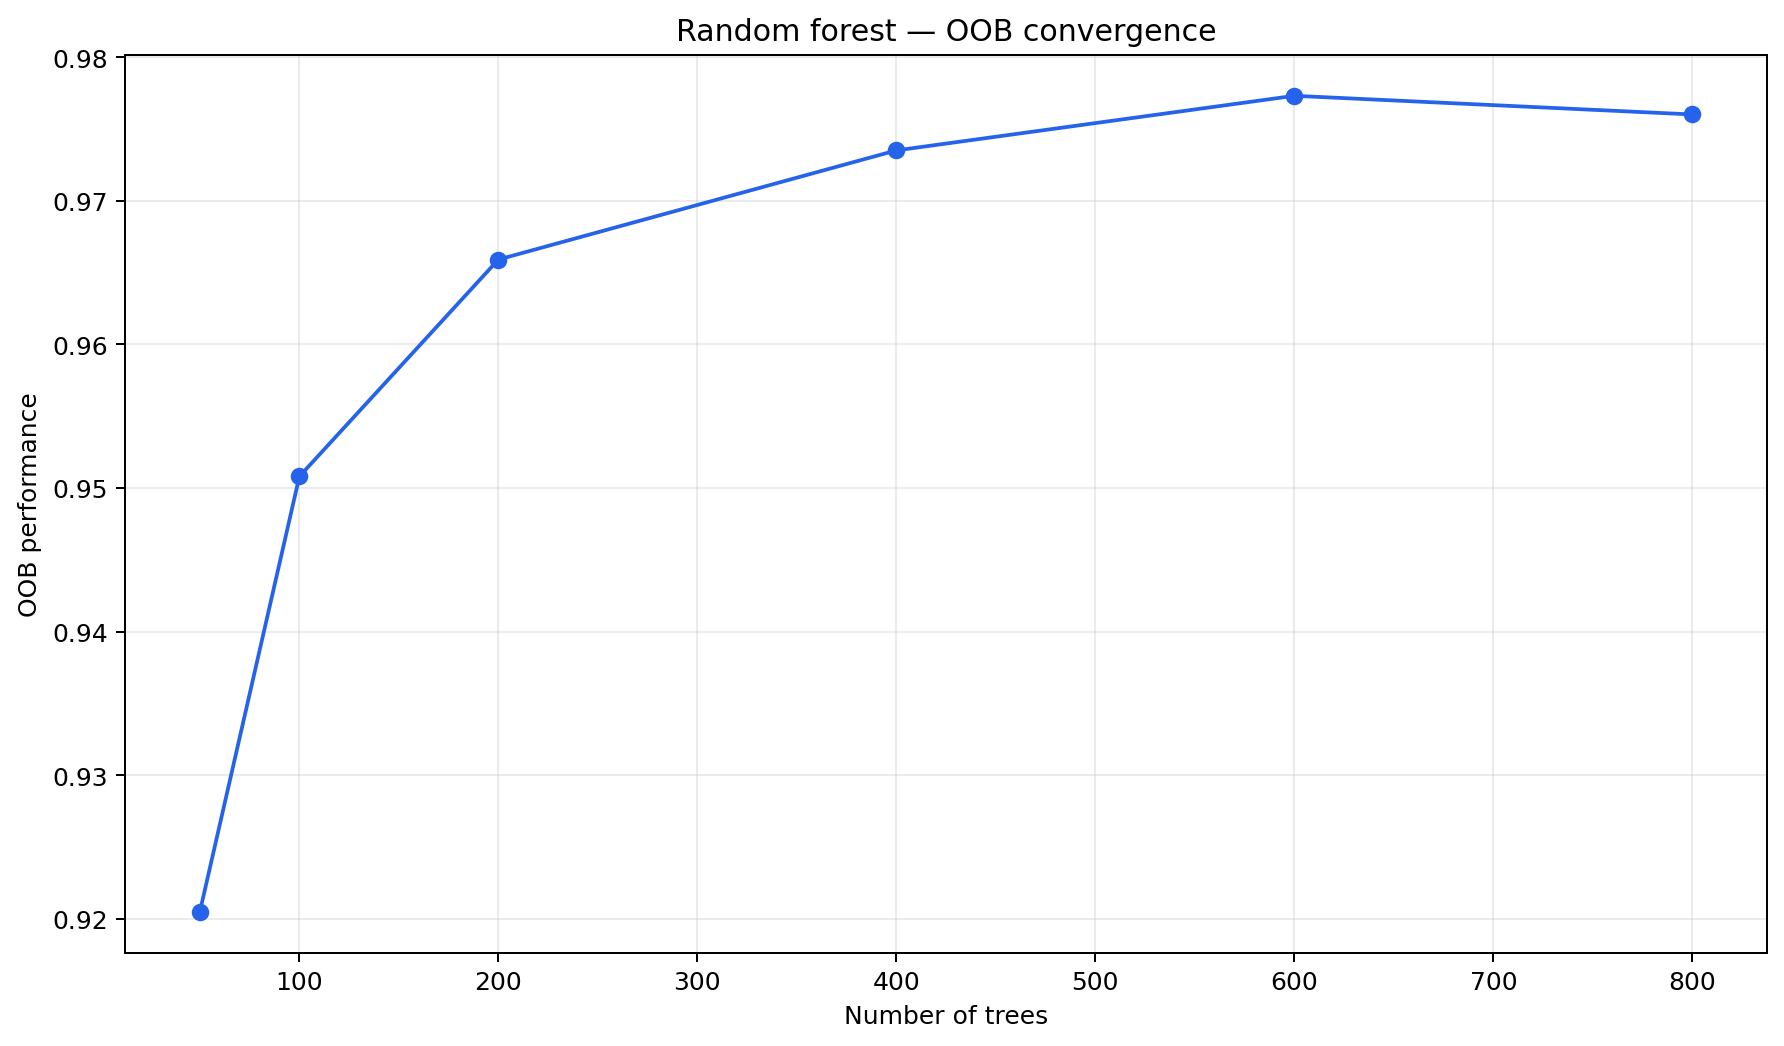
\includegraphics[width=\textwidth]{../figures/en/fig10_oob_vs_n_estimators.png}
\caption{Exploratory evolution of the OOB score with the number of trees. The curve suggests that performance stabilizes quickly once the forest is sufficiently large.}
\end{figure}

\begin{figure}[H]
\centering
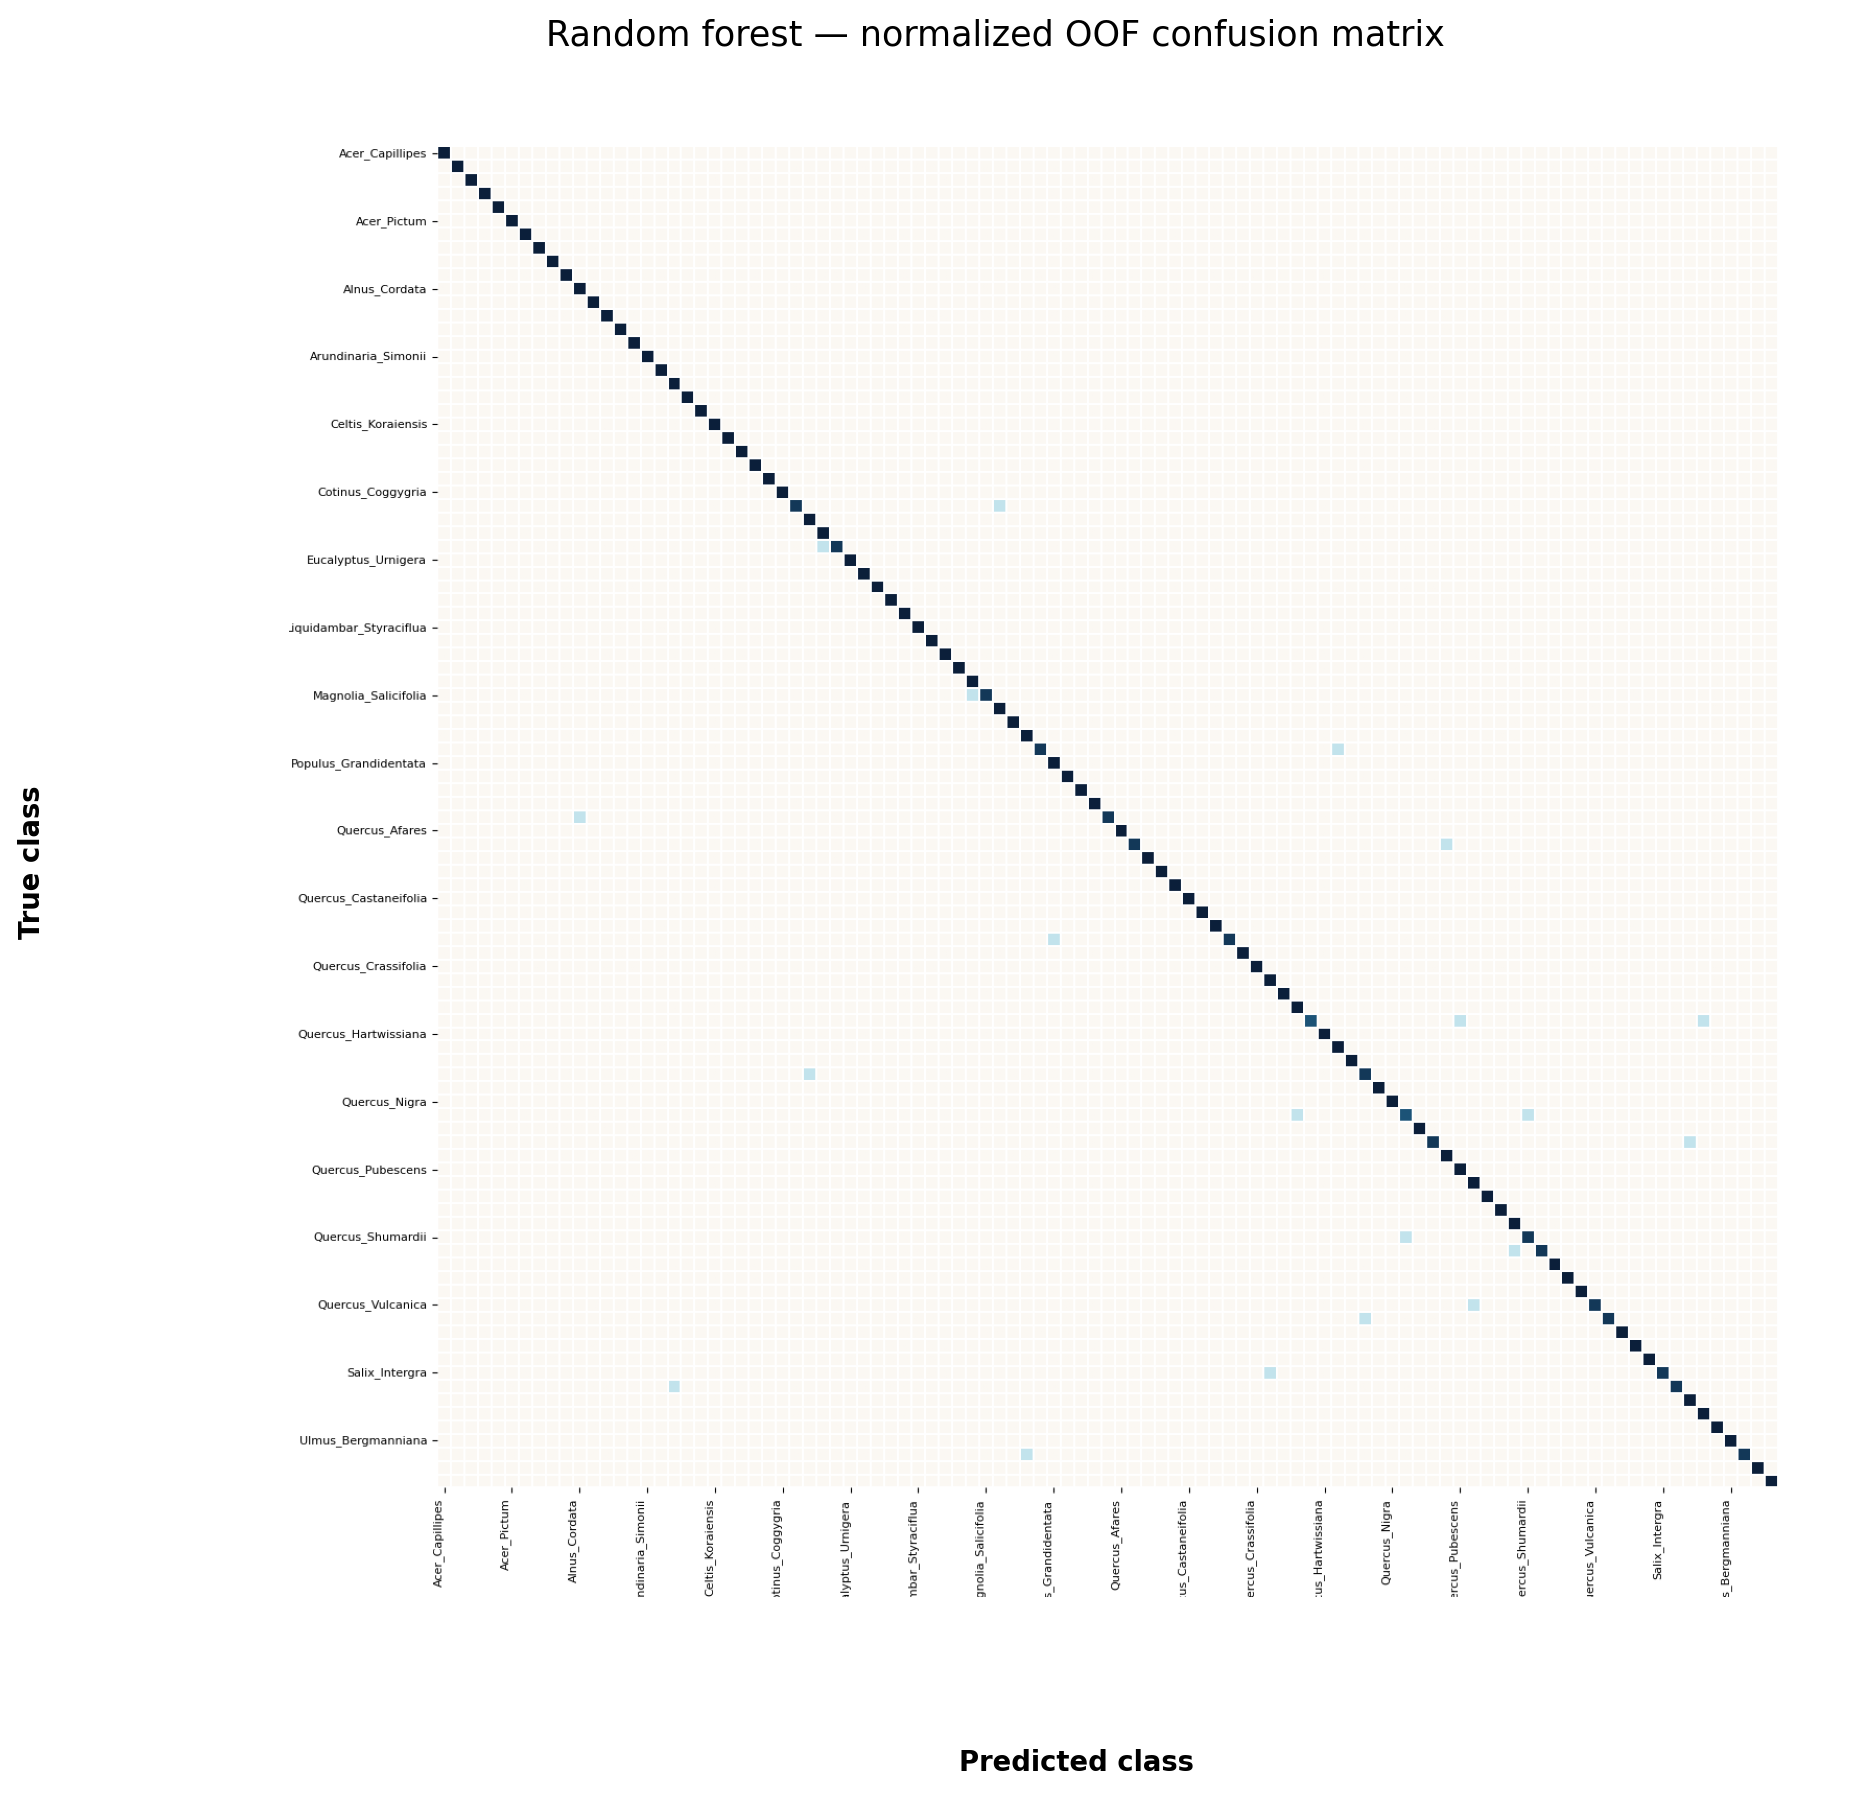
\includegraphics[width=\textwidth]{../figures/en/figA_confusion_rf_tuned.png}
\caption{Normalized confusion matrix obtained from the out-of-fold predictions of the \texttt{tuned} variant. The pattern remains very close to that of the project's best models.}
\end{figure}

\begin{figure}[H]
\centering
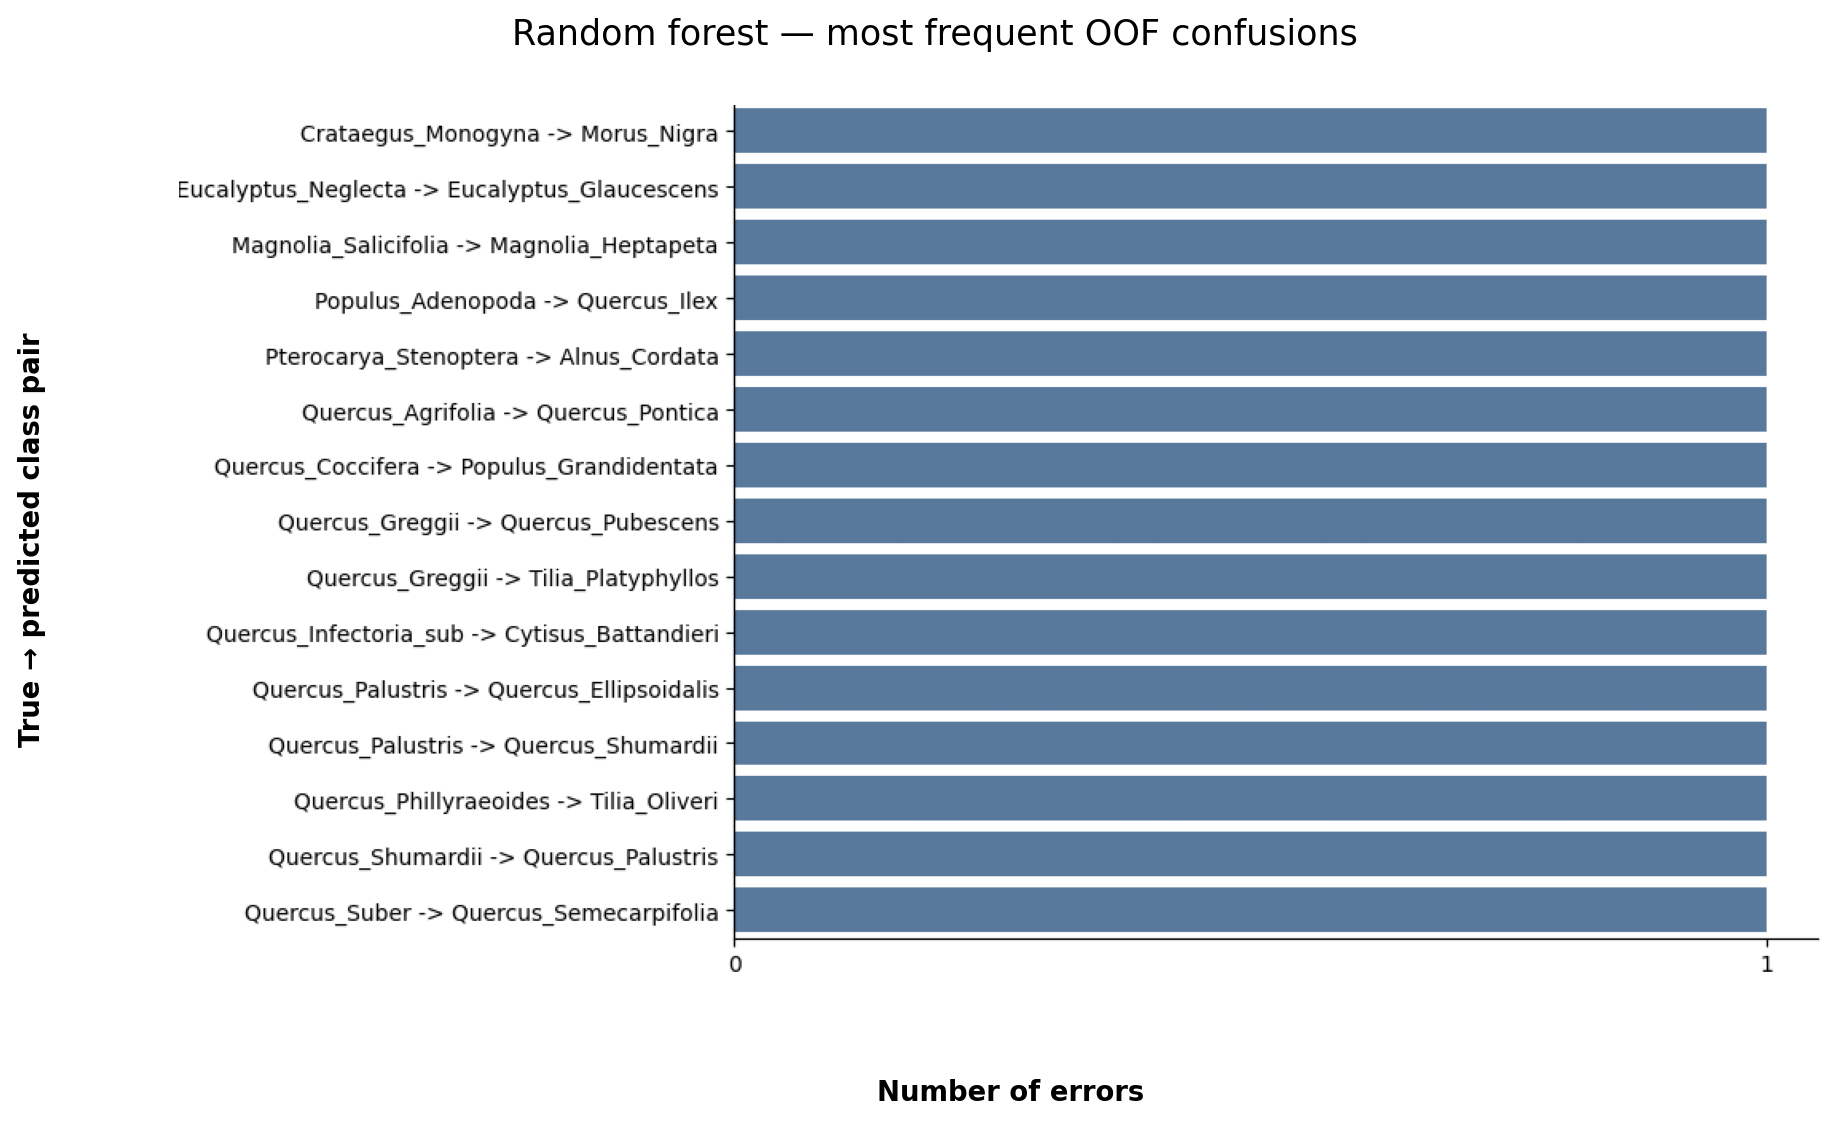
\includegraphics[width=\textwidth]{../figures/en/fig_rf_top12_confusions.png}
\caption{Leading residual confusions for the random forest. Their limited number confirms the problem's strong effective separability for this family.}
\end{figure}

\subsubsection{Secondary corroboration}
Secondary corroboration is available on the frozen split. The selected reference is the \texttt{default} variant, chosen from the exploratory results on the development set. On the corroboration set, \texttt{default} and \texttt{tuned} obtain exactly the same scores: \texttt{0.9842} in \texttt{F1-macro} and \texttt{0.9848} in \texttt{accuracy}. The \texttt{tuned - reference} delta is therefore zero.

\begin{table}[H]
\centering
\begin{tabular}{|l|r|r|l|}
\hline
\textbf{Variant} & \textbf{Corroboration F1} & \textbf{Corroboration accuracy} & \textbf{Role} \\
\hline
\texttt{default} & \texttt{0.9842} & \texttt{0.9848} & reference \\
\texttt{restricted\_depth} & \texttt{0.9468} & \texttt{0.9545} & descriptive \\
\texttt{tuned} & \texttt{0.9842} & \texttt{0.9848} & tuned \\
\hline
\end{tabular}
\end{table}

Here, corroboration confirms the family's excellent performance without providing clear evidence of an additional gain from tuning. The random forest therefore remains a leading, robust, and highly effective model, although its default configuration is already close to the practical optimum on this dataset.

\begin{figure}[H]
\centering
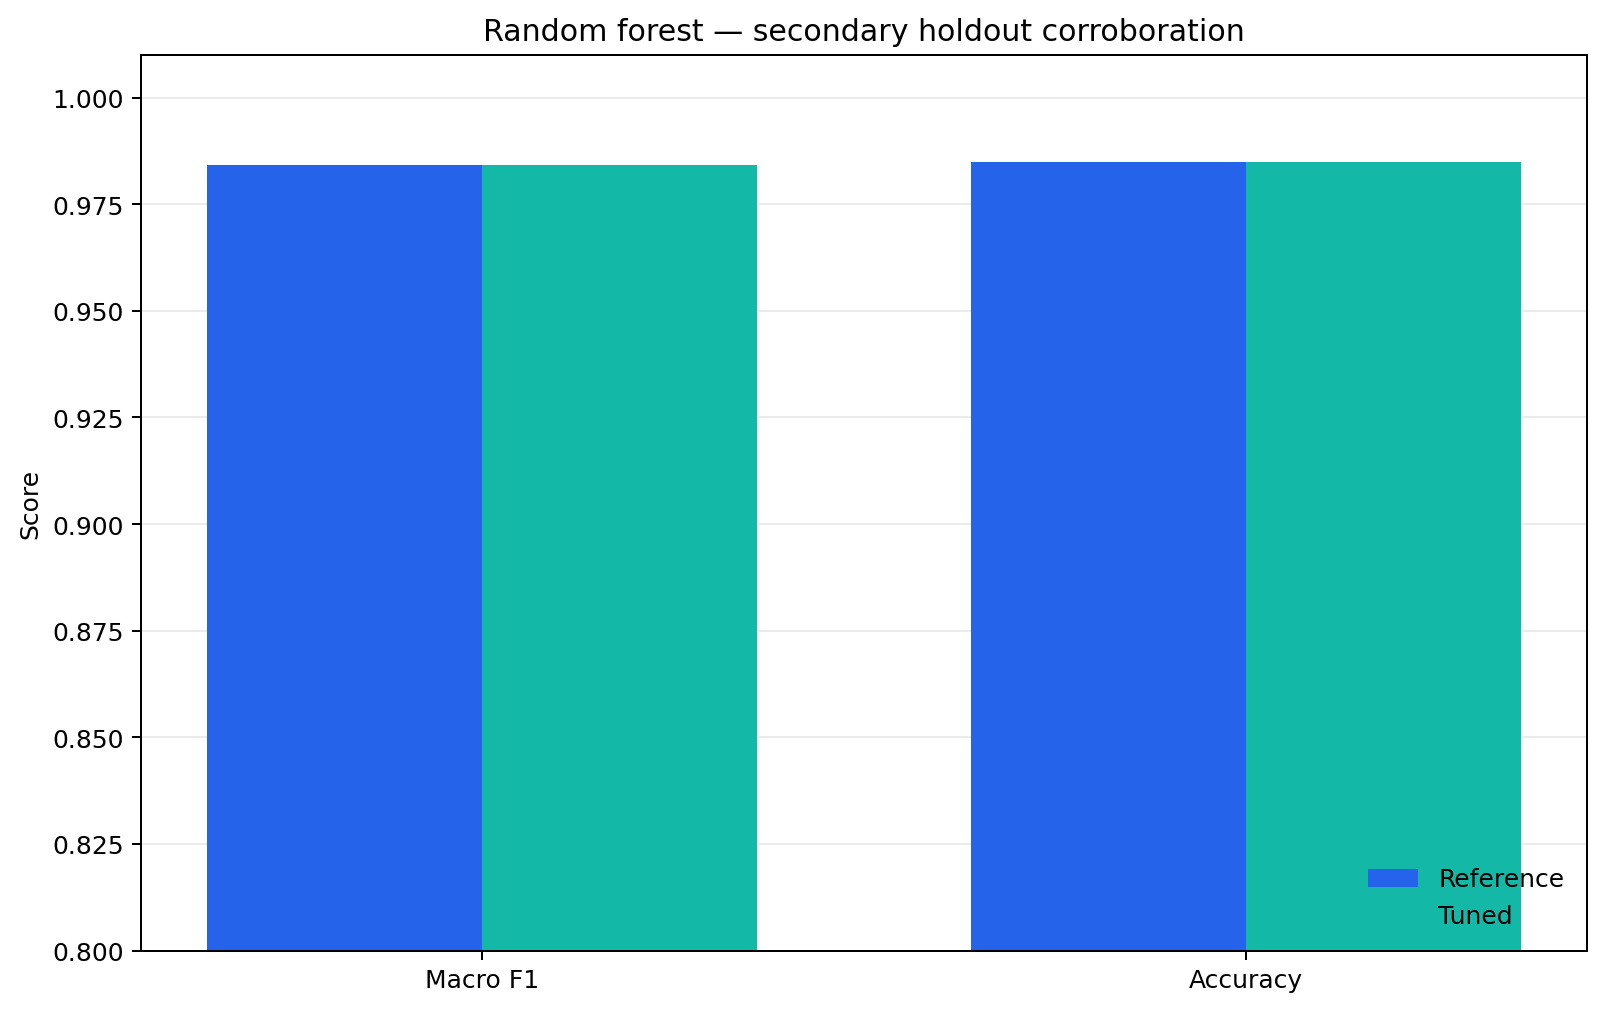
\includegraphics[width=\textwidth]{../figures/en/fig_rf_corroboration_holdout.png}
\caption{Secondary comparison between the reference and \texttt{tuned} random-forest variants on the corroboration set.}
\end{figure}

% --- DECISION TREE ---
\subsection{Decision tree model}

\subsubsection{Role of the model}
The decision tree is studied here less as a final candidate than as a reference point for the tradeoff between interpretability and generalization. This family makes the effects of depth, leaf size, and pruning directly observable, but is also particularly prone to overfitting in a rich multiclass problem.

\subsubsection{Exploration}
The two exploratory variants clearly bracket the family's behavior. The \texttt{default} variant achieves \texttt{0.5809} in \texttt{F1-macro} and \texttt{0.6174} in \texttt{accuracy}, but with a very high generalization gap (\texttt{0.4191}). Conversely, \texttt{restricted\_depth} sharply reduces this gap (\texttt{0.0797}) at the cost of a collapse in performance, reaching only \texttt{0.1468} in \texttt{F1-macro}.

\begin{table}[H]
\centering
\begin{tabular}{|l|l|r|r|r|r|}
\hline
\textbf{Variant} & \textbf{Protocol} & \textbf{Macro F1} & \textbf{Accuracy} & \textbf{F1 gap} & \textbf{Time (s)} \\
\hline
\texttt{default} & simple CV & \texttt{0.5809} & \texttt{0.6174} & \texttt{0.4191} & \texttt{1.04} \\
\texttt{restricted\_depth} & simple CV & \texttt{0.1468} & \texttt{0.1529} & \texttt{0.0797} & \texttt{0.56} \\
\hline
\end{tabular}
\end{table}

The exploratory conclusion is unambiguous: an overly flexible tree memorizes the data, while an overly constrained tree loses most of its discriminative power. A useful region exists for the family, but it appears narrow and unstable.

\begin{figure}[H]
\centering
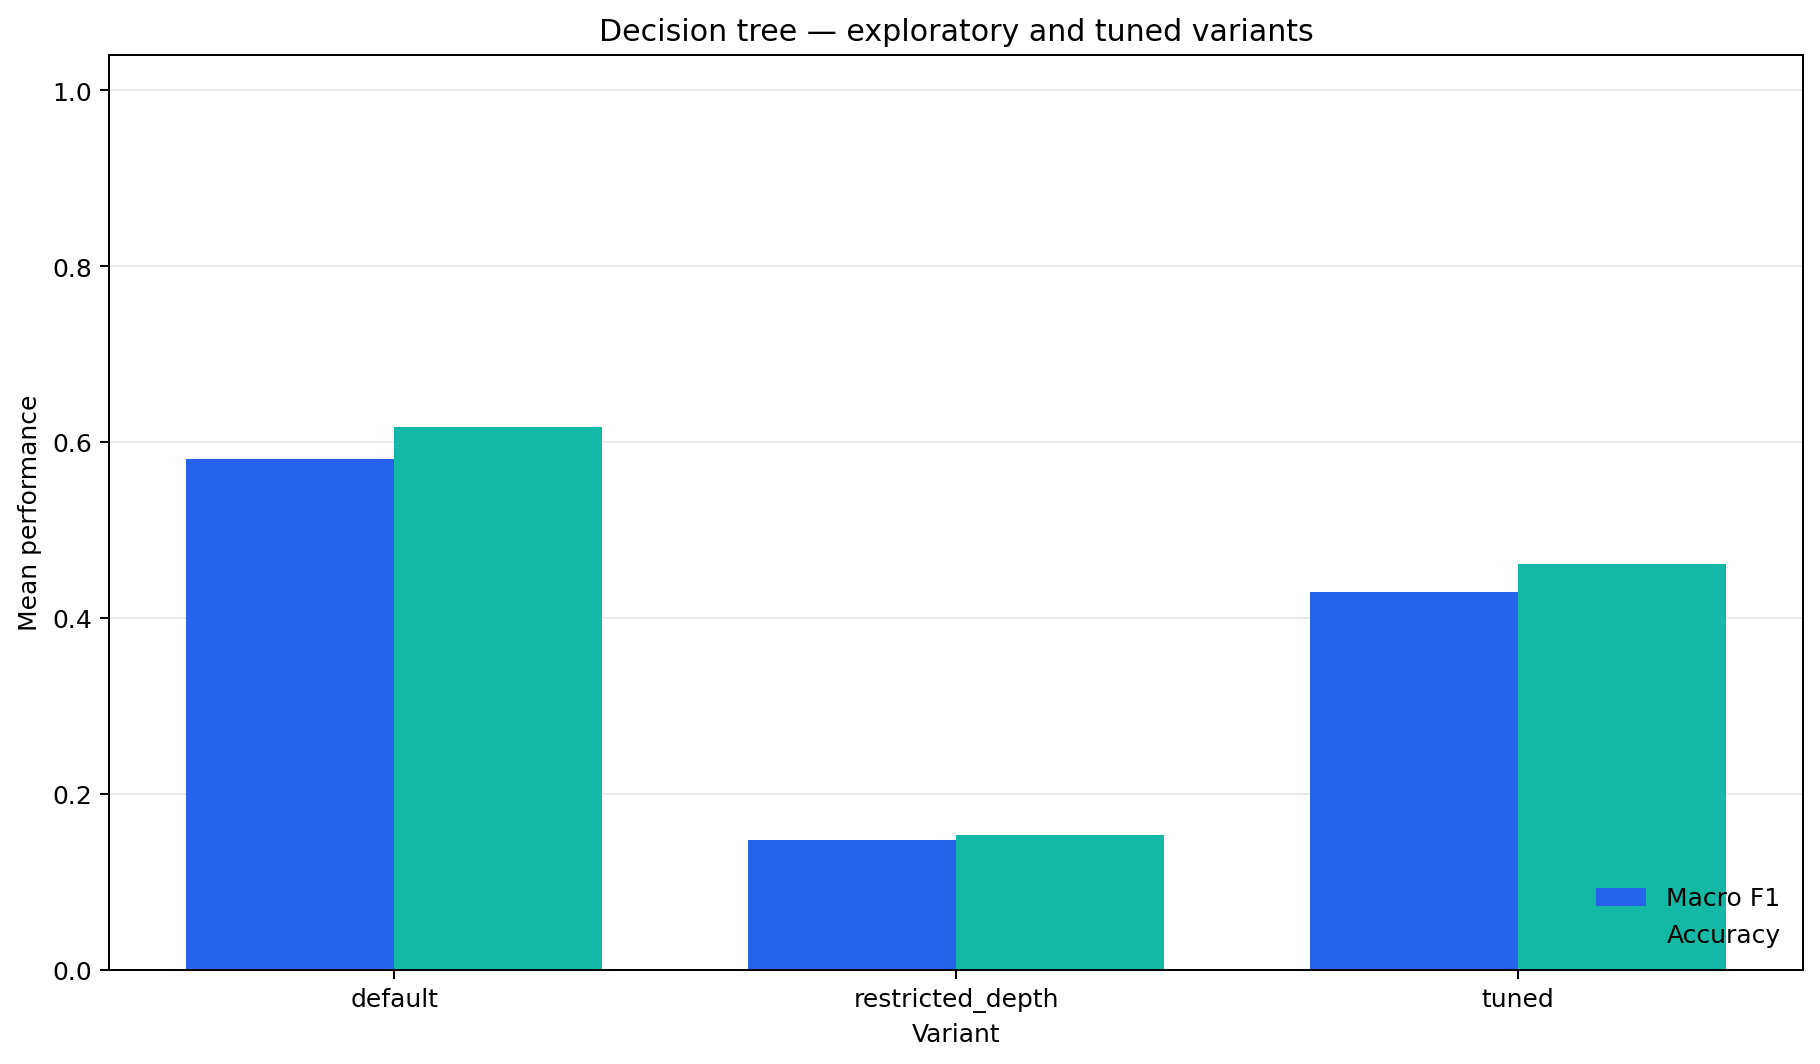
\includegraphics[width=\textwidth]{../figures/en/fig_dt_comparaison_variantes.png}
\caption{Exploratory comparison of decision-tree variants. The performance--complexity tradeoff remains generally unfavorable for a single tree.}
\end{figure}

\subsubsection{Confirmation}
Nested cross-validation confirms this fragility. The \texttt{tuned} variant achieves a mean \texttt{F1-macro} of \texttt{0.4295} and mean \texttt{accuracy} of \texttt{0.4610}, with standard deviations of \texttt{0.0546} and \texttt{0.0627}. The decline relative to the \texttt{default} variant does not mean that tuning degrades the model; rather, it indicates that a stricter confirmatory estimate corrects the optimism of simple evaluation for a highly unstable estimator.

\begin{table}[H]
\centering
\begin{tabular}{|l|r|}
\hline
\textbf{Confirmatory metric} & \textbf{Value} \\
\hline
Mean Macro F1 & \texttt{0.4295} \\
F1 standard deviation & \texttt{0.0546} \\
Mean accuracy & \texttt{0.4610} \\
Accuracy standard deviation & \texttt{0.0627} \\
Protocol & \texttt{nested CV} \\
Outer folds & \texttt{5} \\
Inner folds & \texttt{3} \\
Total time (s) & \texttt{11.47} \\
\hline
\end{tabular}
\end{table}

The decision tree therefore ranks far behind the other families. It remains pedagogically useful for examining the mechanisms of overfitting, but it is not a competitive solution in this project.

\subsubsection{Descriptive diagnostics}
The validation curve for \texttt{max\_depth} directly exposes the core problem: the training score rises quickly with depth, whereas the validation score plateaus and then deteriorates. Accordingly, the confusion matrices show a much more diffuse pattern than those of the best-performing models.

\begin{figure}[H]
\centering
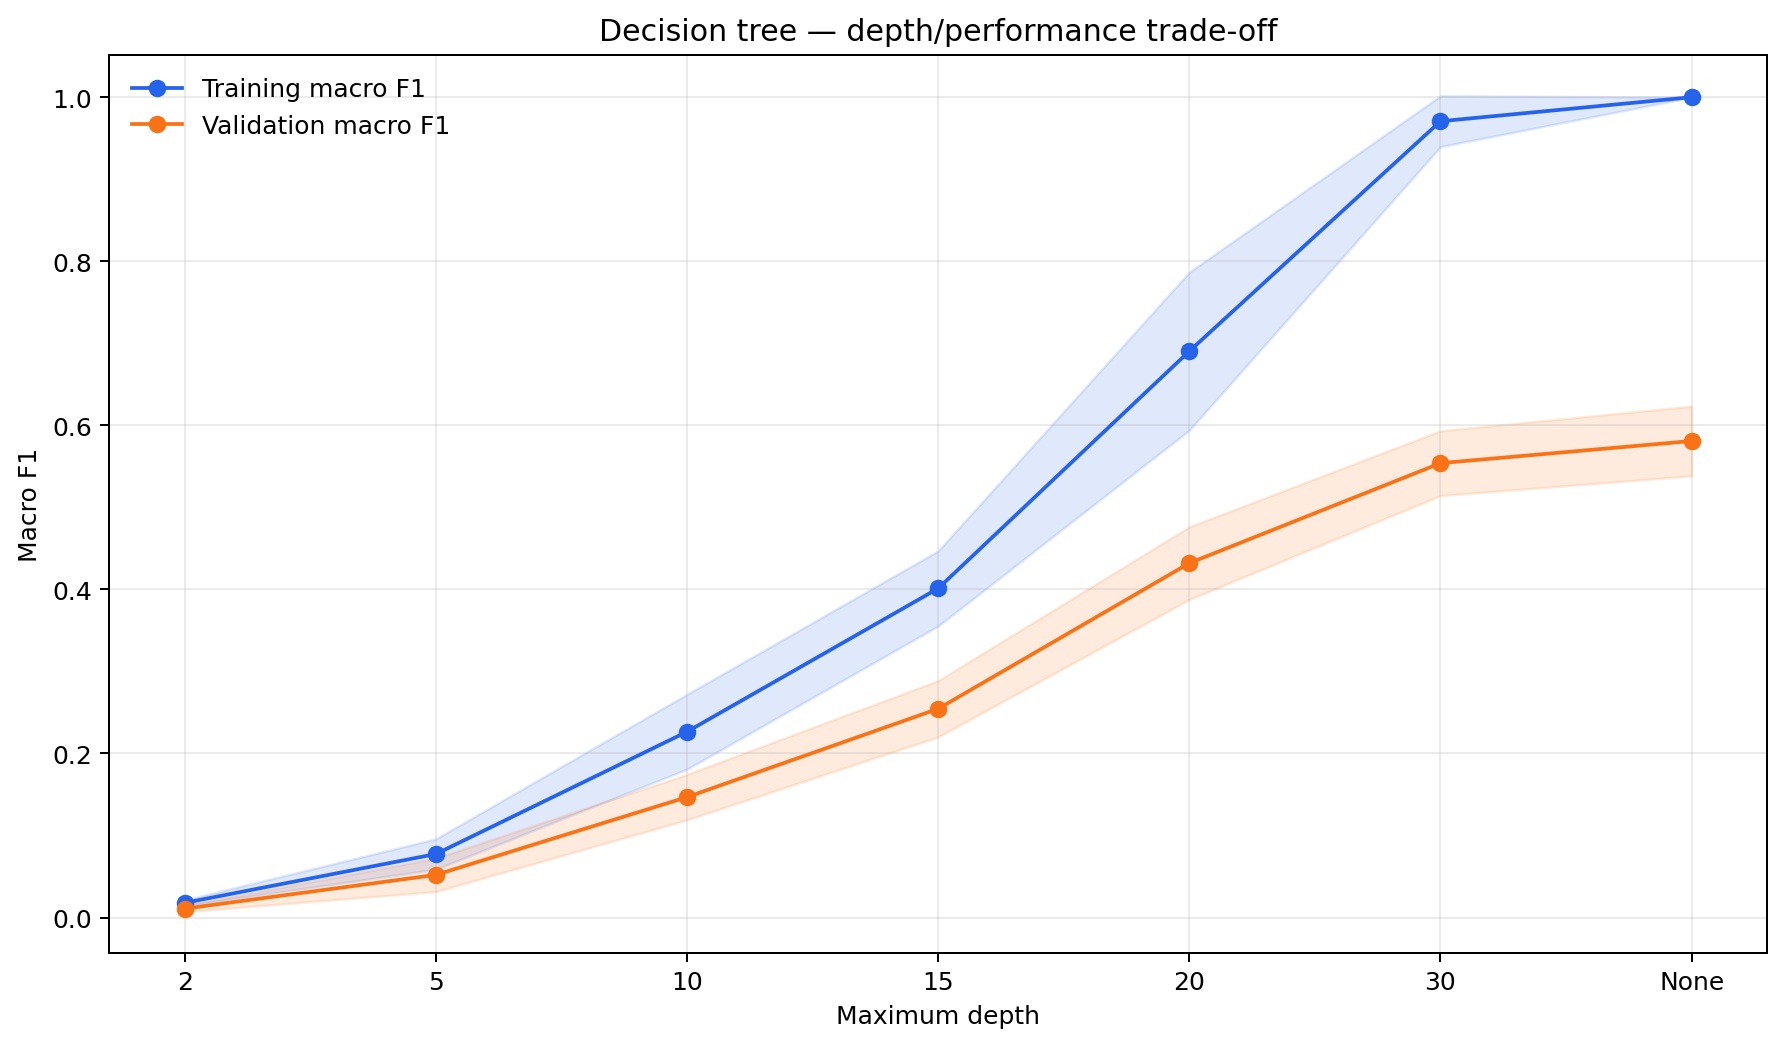
\includegraphics[width=\textwidth]{../figures/en/figA3_validation_curve_max_depth.png}
\caption{Exploratory validation curve for \texttt{max\_depth}. The divergence between training and validation directly illustrates the family's fragility.}
\end{figure}

\begin{figure}[H]
\centering
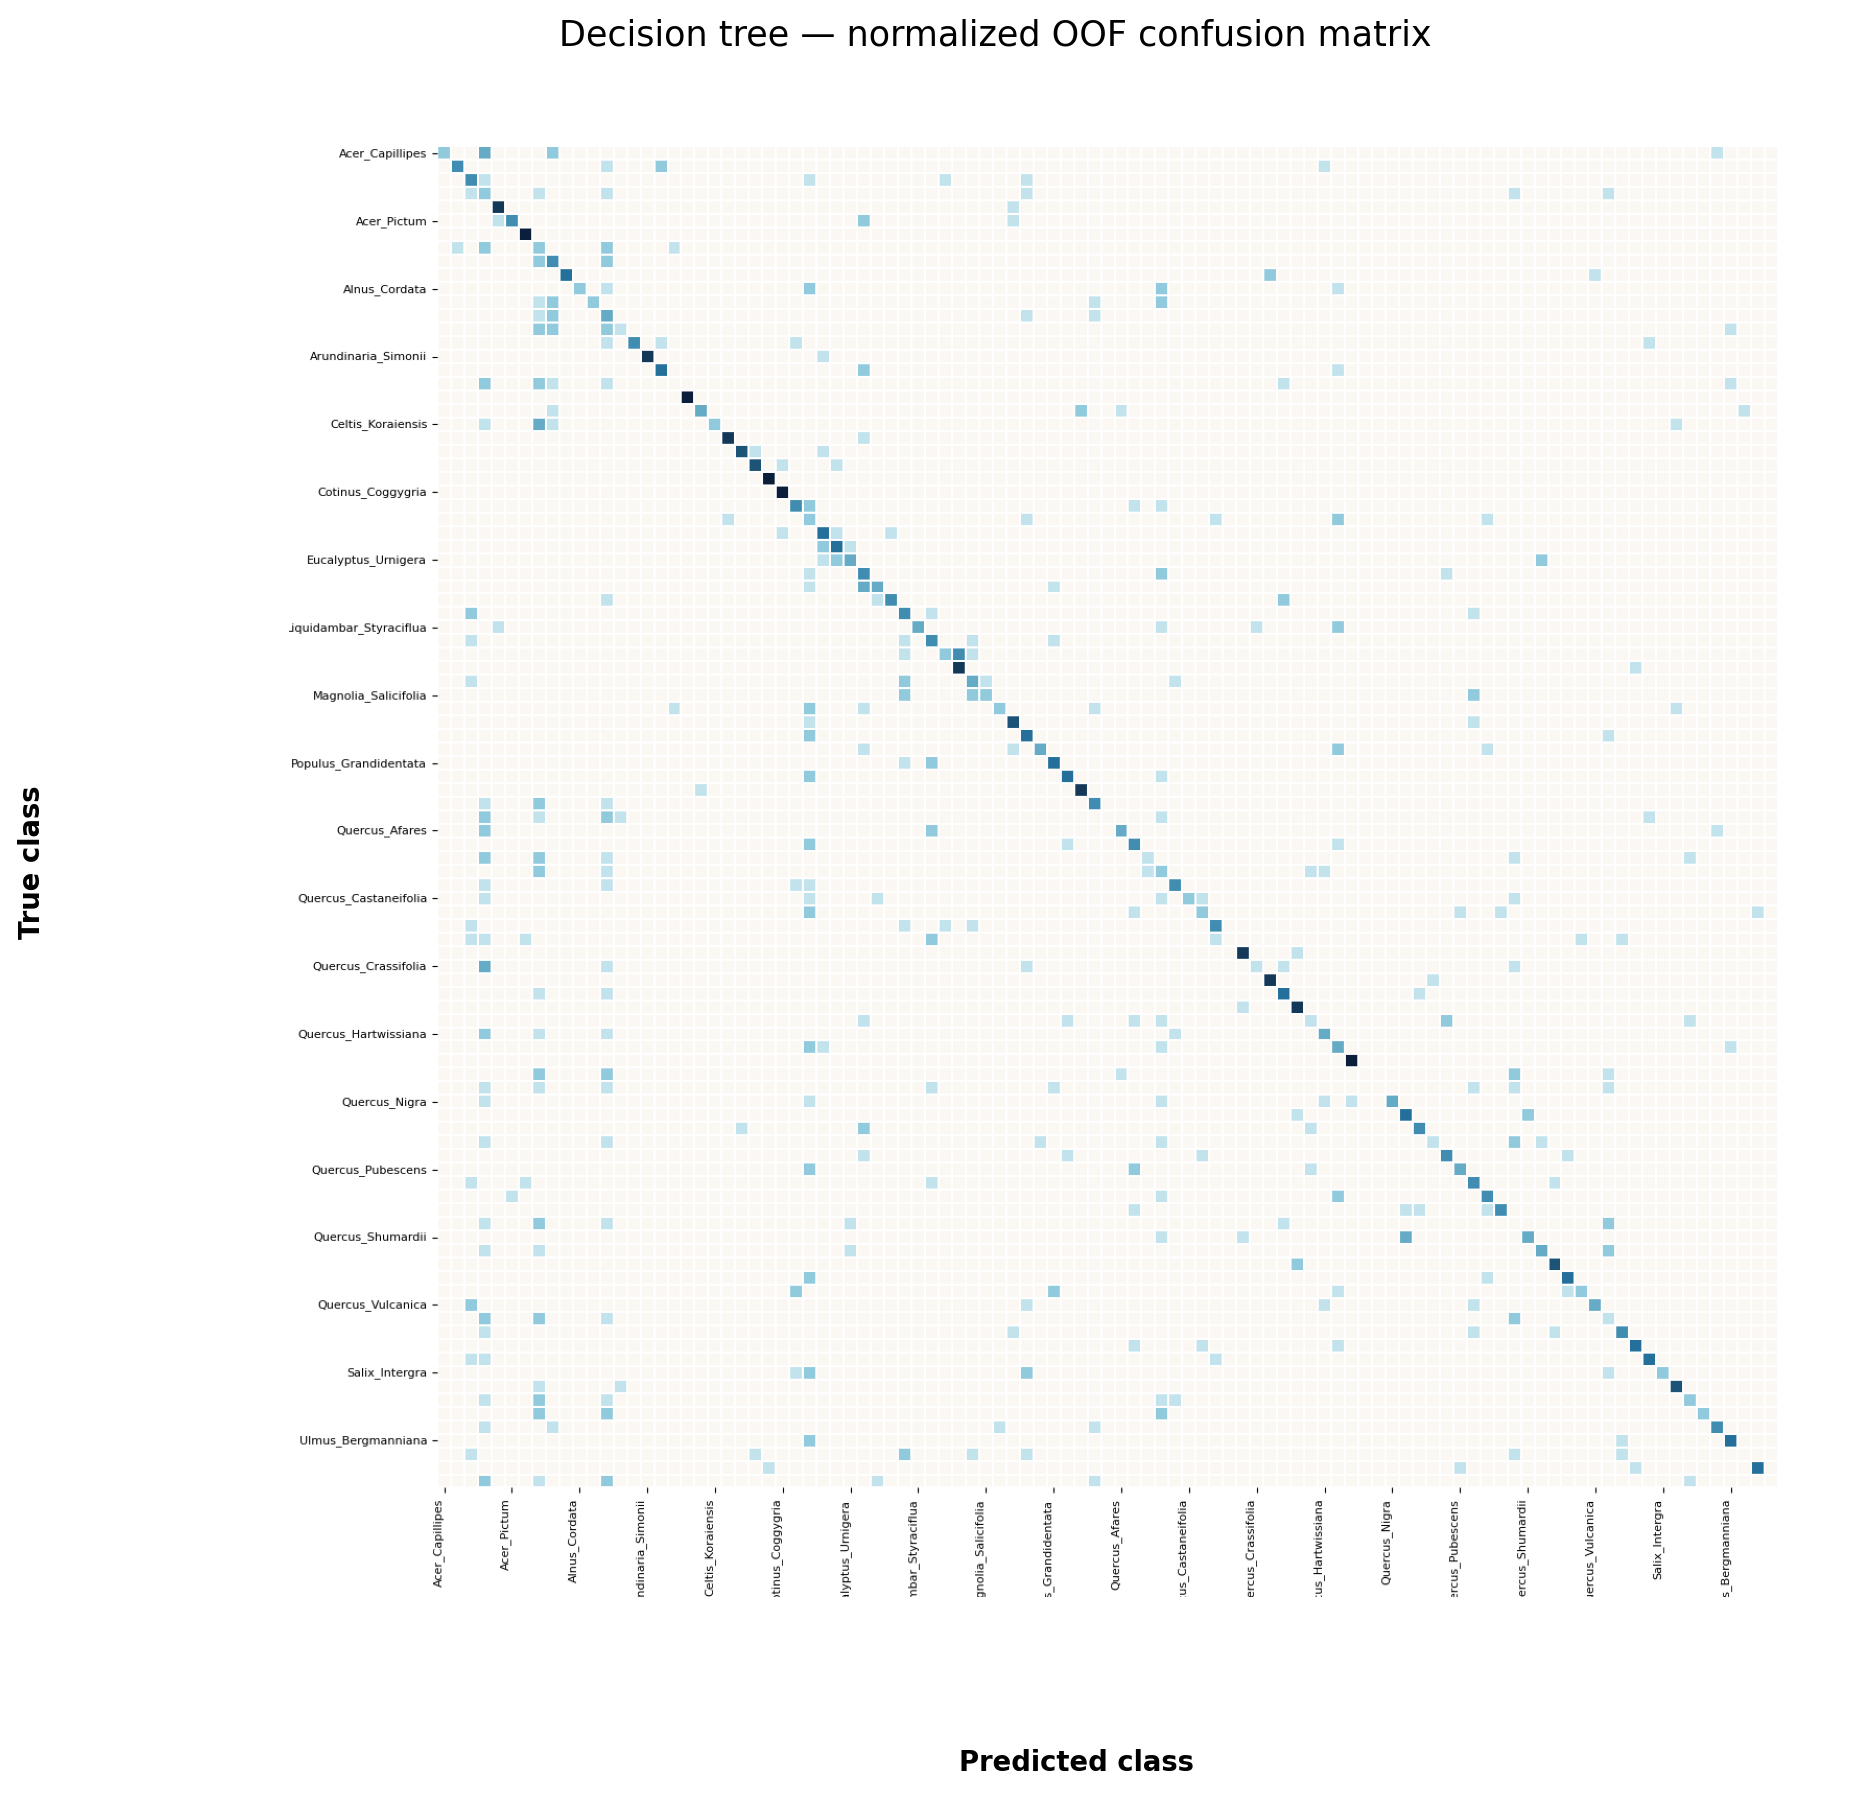
\includegraphics[width=\textwidth]{../figures/en/figA_confusion_dt_tuned.png}
\caption{Normalized confusion matrix from the out-of-fold predictions of the \texttt{tuned} variant. Errors remain numerous and dispersed.}
\end{figure}

\begin{figure}[H]
\centering
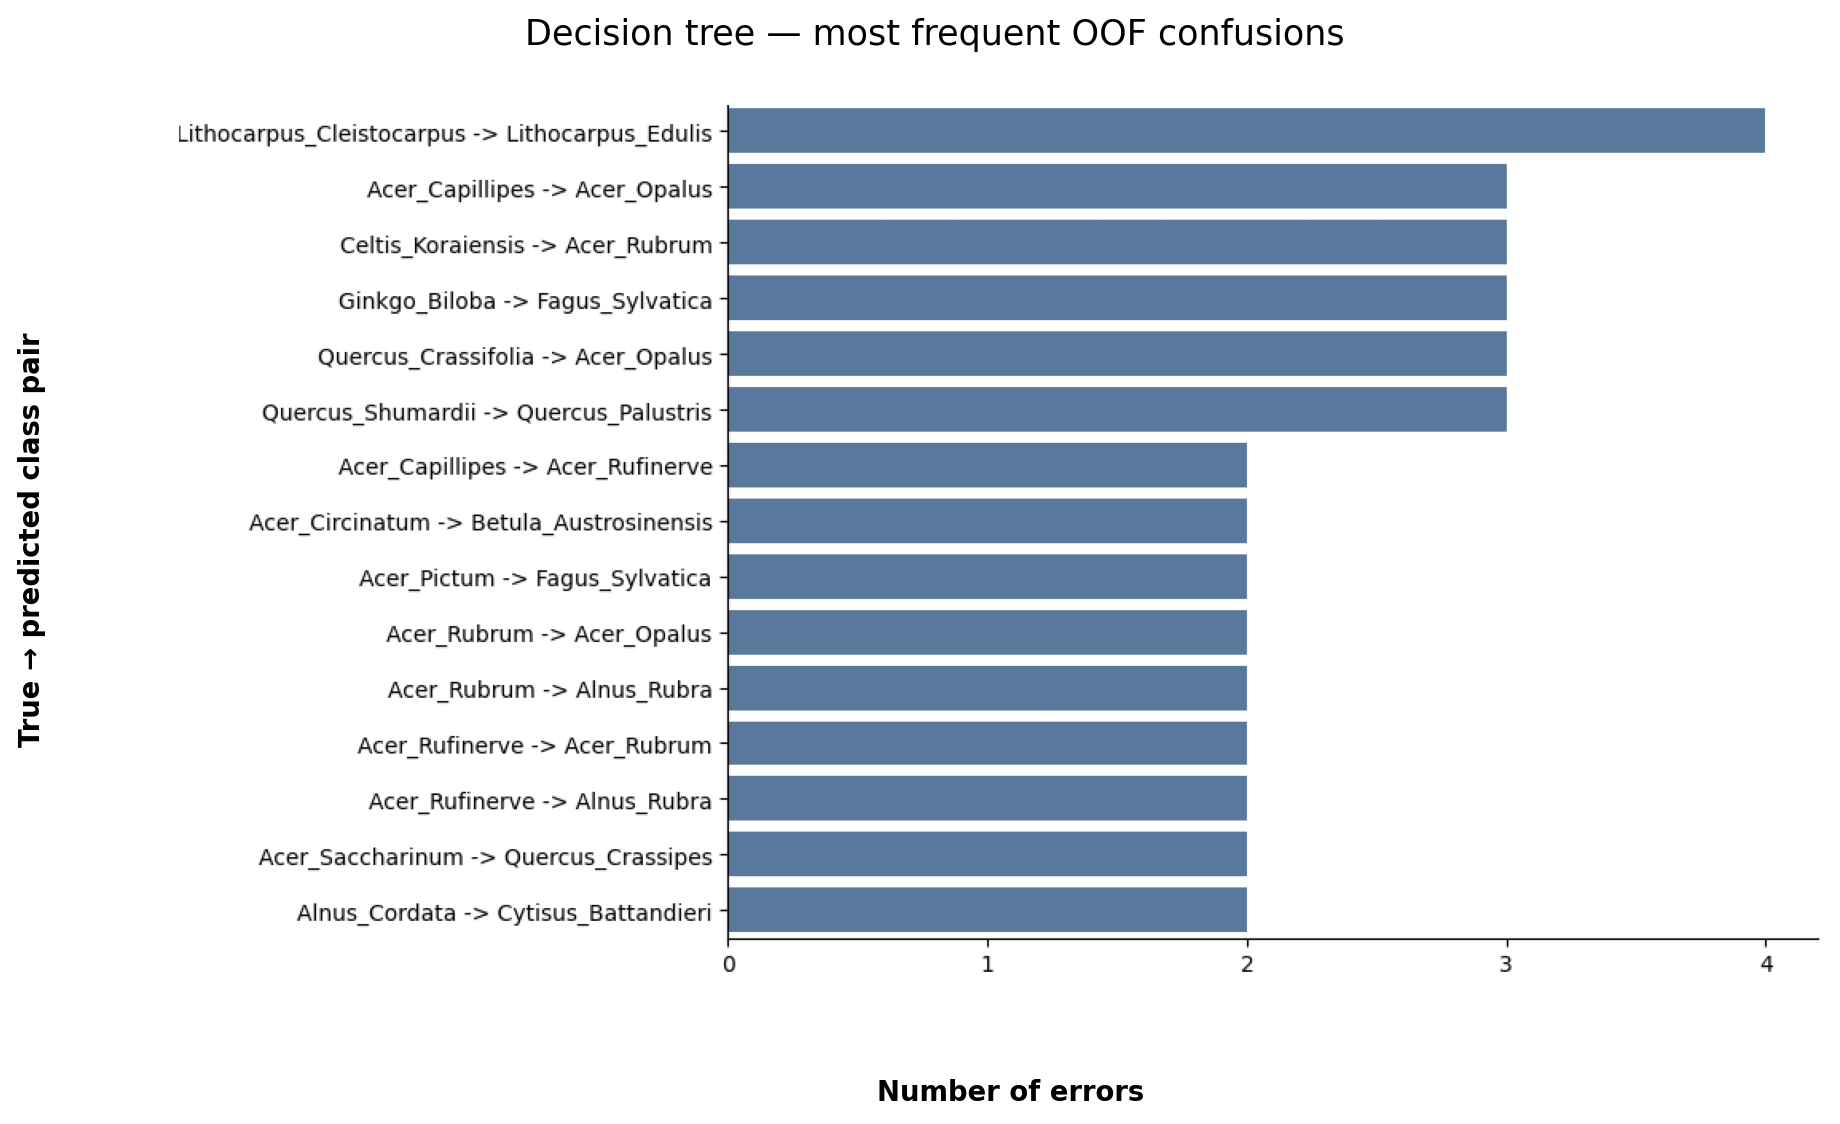
\includegraphics[width=\textwidth]{../figures/en/fig_dt_top12_confusions.png}
\caption{Leading confusions for the tuned decision tree. Their dispersion is consistent with insufficient generalization on a problem with \texttt{99} classes.}
\end{figure}

\subsubsection{No secondary corroboration}
Unlike the other eligible families, no secondary corroboration is published for the decision tree in the canonical artifacts. The scientific interpretation therefore rests solely on the relationship among exploration, confirmation, and confusion diagnostics.

This absence does not change the substantive conclusion. Even without secondary corroboration, the confirmatory results are sufficient to show that a single tree remains too unstable to compete with regularized linear models, the SVM, the random forest, or even the MLP.

% --- MLP ---
\subsection{MLP model}

\subsubsection{Role of the model}
The MLP represents the study's dense neural-network family. It tests whether a nonlinear capacity more flexible than linear or kernel models produces an empirical gain on a moderately sized tabular dataset with relatively few examples per class.

\subsubsection{Exploration}
The exploratory stage shows very clearly that preprocessing is a prerequisite for this model to function effectively. Without scaling, the MLP collapses to \texttt{0.1642} in \texttt{F1-macro} and \texttt{0.1863} in \texttt{accuracy}, with very high variability. Once the variables are standardized, the \texttt{scaled\_only} variant reaches \texttt{0.9389} in \texttt{F1-macro} and \texttt{0.9482} in \texttt{accuracy}, while \texttt{scaled\_pca} reaches \texttt{0.9323} and \texttt{0.9444}.

\begin{table}[H]
\centering
\begin{tabular}{|l|l|r|r|r|r|}
\hline
\textbf{Variant} & \textbf{Protocol} & \textbf{Macro F1} & \textbf{Accuracy} & \textbf{F1 gap} & \textbf{Time (s)} \\
\hline
\texttt{default} & simple CV & \texttt{0.1642} & \texttt{0.1863} & \texttt{0.0262} & \texttt{1.97} \\
\texttt{scaled\_only} & simple CV & \texttt{0.9389} & \texttt{0.9482} & \texttt{0.0552} & \texttt{2.01} \\
\texttt{scaled\_pca} & simple CV & \texttt{0.9323} & \texttt{0.9444} & \texttt{0.0604} & \texttt{1.97} \\
\hline
\end{tabular}
\end{table}

The central diagnosis is therefore clear: the MLP becomes competitive only when supplied through a strict standardization pipeline. \texttt{PCA} provides no clear benefit and remains slightly behind the \texttt{scaled\_only} variant.

\begin{figure}[H]
\centering
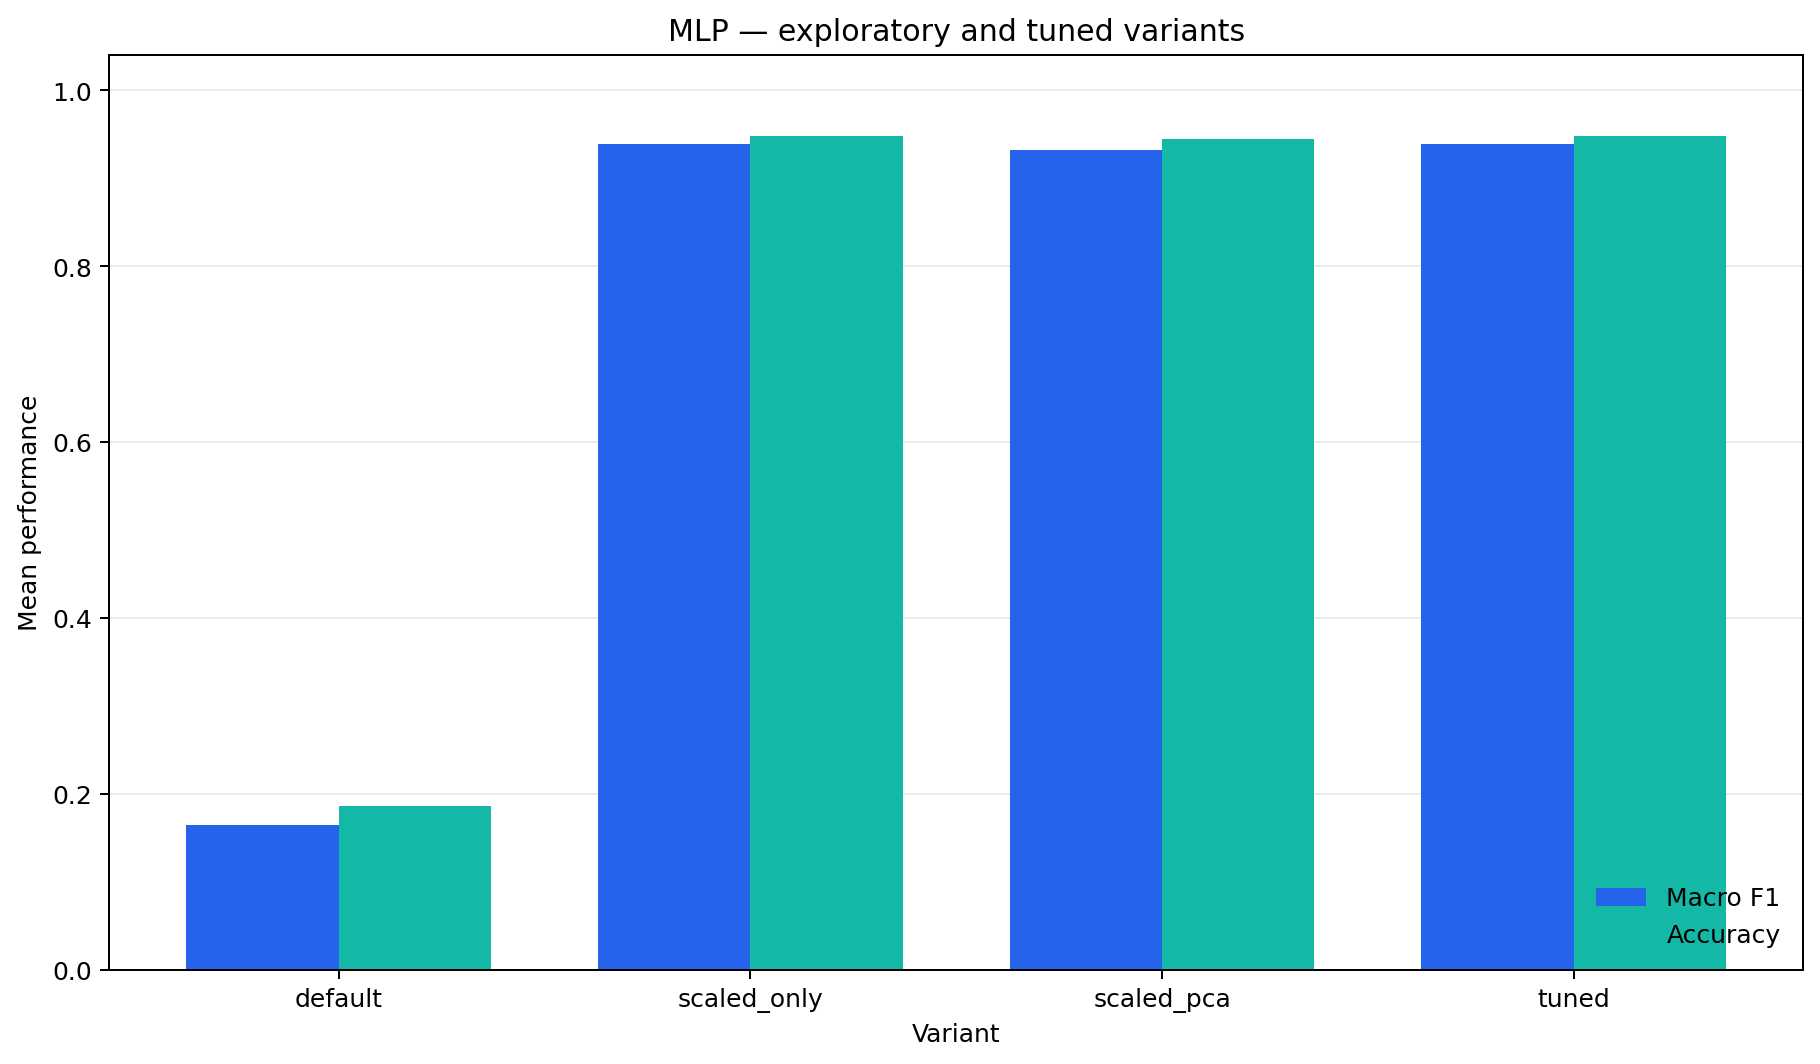
\includegraphics[width=\textwidth]{../figures/en/fig_mlp_comparaison_variantes.png}
\caption{Exploratory comparison of MLP variants. The contrast between the raw and scaled versions illustrates the network's dependence on feature scale.}
\end{figure}

\subsubsection{Confirmation}
Confirmatory evaluation yields a mean \texttt{F1-macro} of \texttt{0.9389} and mean \texttt{accuracy} of \texttt{0.9482}, with standard deviations of \texttt{0.0322} and \texttt{0.0279}. The \texttt{tuned} variant therefore reproduces the best exploratory result almost exactly, suggesting that tuning confirms an already strong configuration rather than providing a substantial gain.

\begin{table}[H]
\centering
\begin{tabular}{|l|r|}
\hline
\textbf{Confirmatory metric} & \textbf{Value} \\
\hline
Mean Macro F1 & \texttt{0.9389} \\
F1 standard deviation & \texttt{0.0322} \\
Mean accuracy & \texttt{0.9482} \\
Accuracy standard deviation & \texttt{0.0279} \\
Protocol & \texttt{nested CV} \\
Outer folds & \texttt{5} \\
Inner folds & \texttt{3} \\
Total time (s) & \texttt{38.25} \\
\hline
\end{tabular}
\end{table}

The MLP thus ranks fourth in the confirmatory comparison. It remains clearly effective, but does not convert its additional flexibility into an advantage over the leading trio of logistic regression, SVM, and random forest.

\subsubsection{Descriptive diagnostics}
The diagnostics associated with the MLP primarily clarify its optimization dynamics. The loss curve indicates proper convergence, while the exploratory tuning table shows that most of the signal comes from hidden-layer size rather than \texttt{alpha}. The \texttt{(128,)} configuration consistently outperforms \texttt{(64,)}, while \texttt{PCA} remains slightly behind. These diagnostics help explain the model's behavior without competing with the confirmatory metrics.

\begin{figure}[H]
\centering
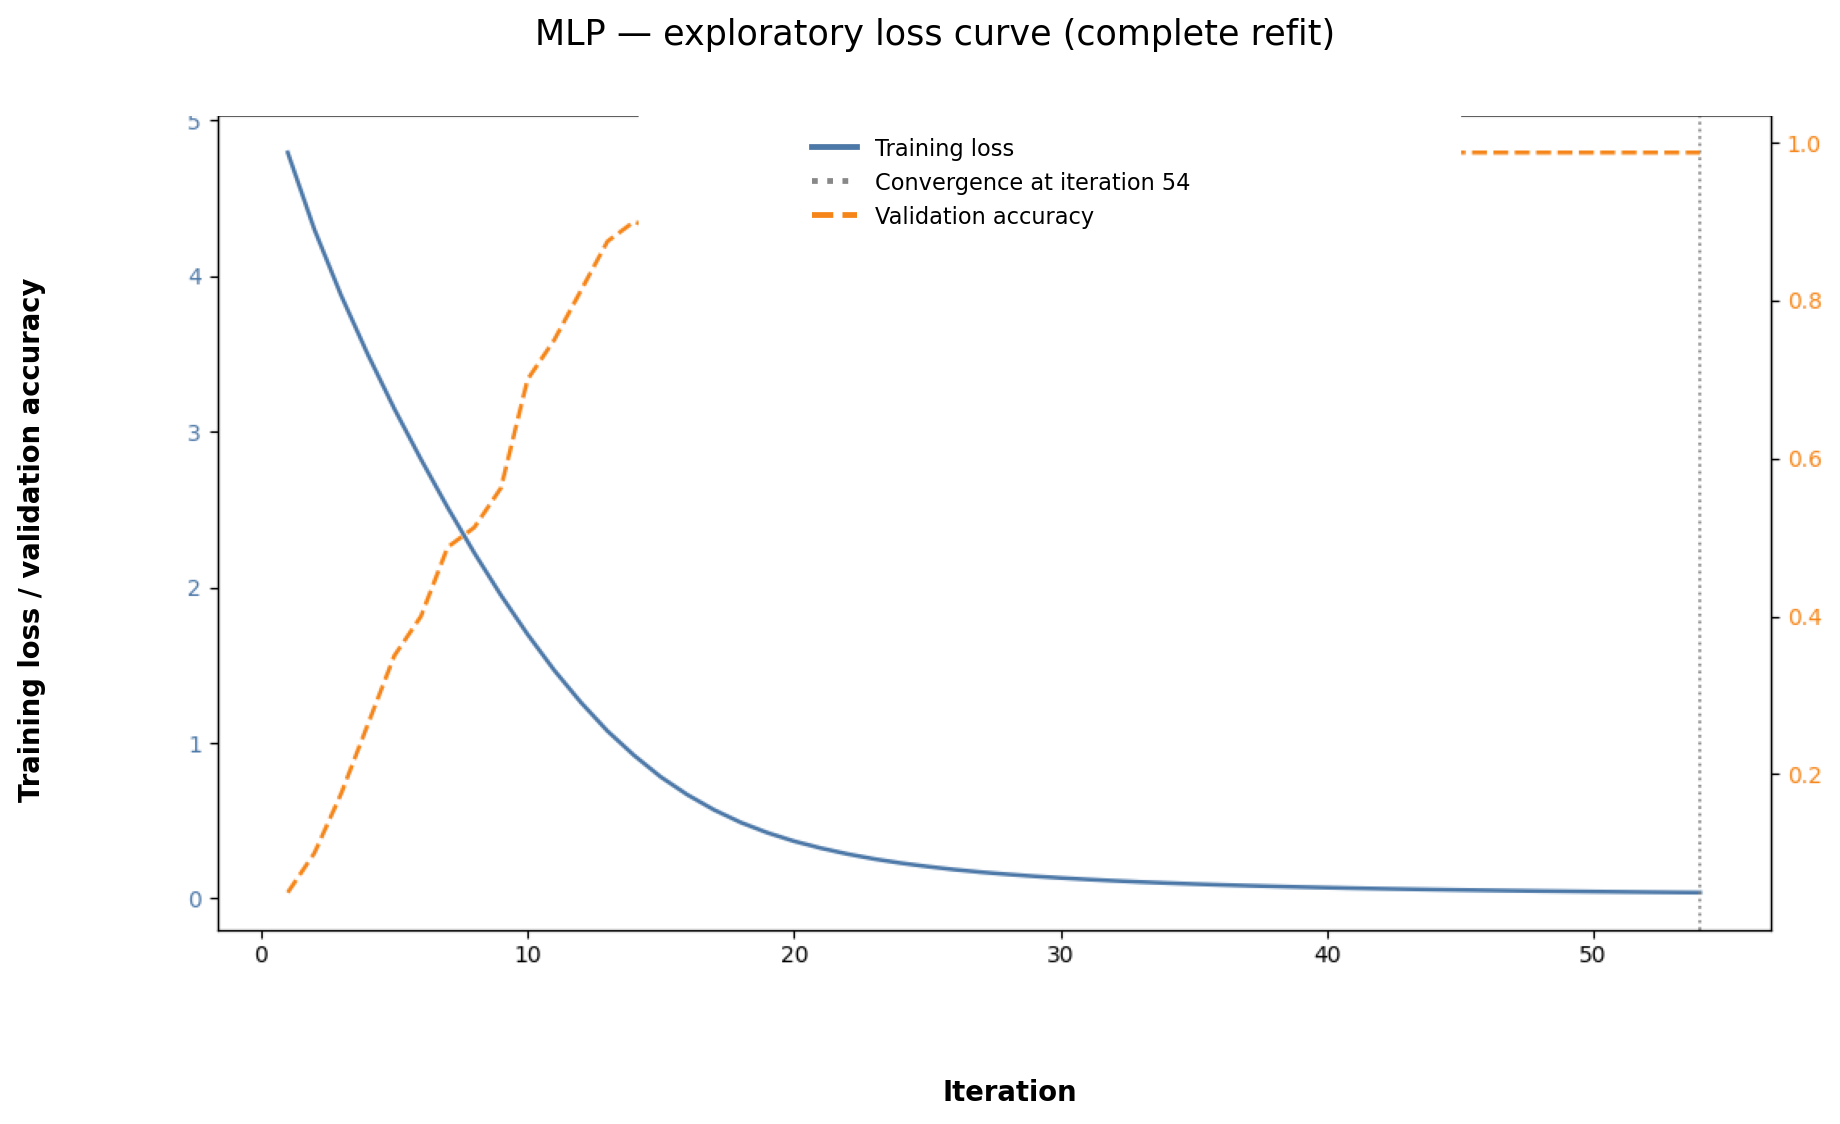
\includegraphics[width=\textwidth]{../figures/en/figA5_loss_curve.png}
\caption{Exploratory diagnostic of MLP convergence. The loss stabilizes properly, although this evidence remains descriptive.}
\end{figure}

\begin{table}[H]
\centering
\begin{tabular}{|l|r|r|}
\hline
\textbf{hidden\_layer\_sizes / alpha} & \textbf{0.0001} & \textbf{0.0010} \\
\hline
\texttt{(64,)} & \texttt{0.9055} & \texttt{0.9055} \\
\texttt{(128,)} & \texttt{0.9341} & \texttt{0.9341} \\
\hline
\end{tabular}
\caption{Exploratory MLP tuning without PCA (mean CV \texttt{F1-macro})}
\end{table}

\begin{table}[H]
\centering
\begin{tabular}{|l|r|r|}
\hline
\textbf{hidden\_layer\_sizes / alpha} & \textbf{0.0001} & \textbf{0.0010} \\
\hline
\texttt{(64,)} & \texttt{0.9107} & \texttt{0.9107} \\
\texttt{(128,)} & \texttt{0.9266} & \texttt{0.9266} \\
\hline
\end{tabular}
\caption{Exploratory MLP tuning with PCA (mean CV \texttt{F1-macro})}
\end{table}

\begin{figure}[H]
\centering
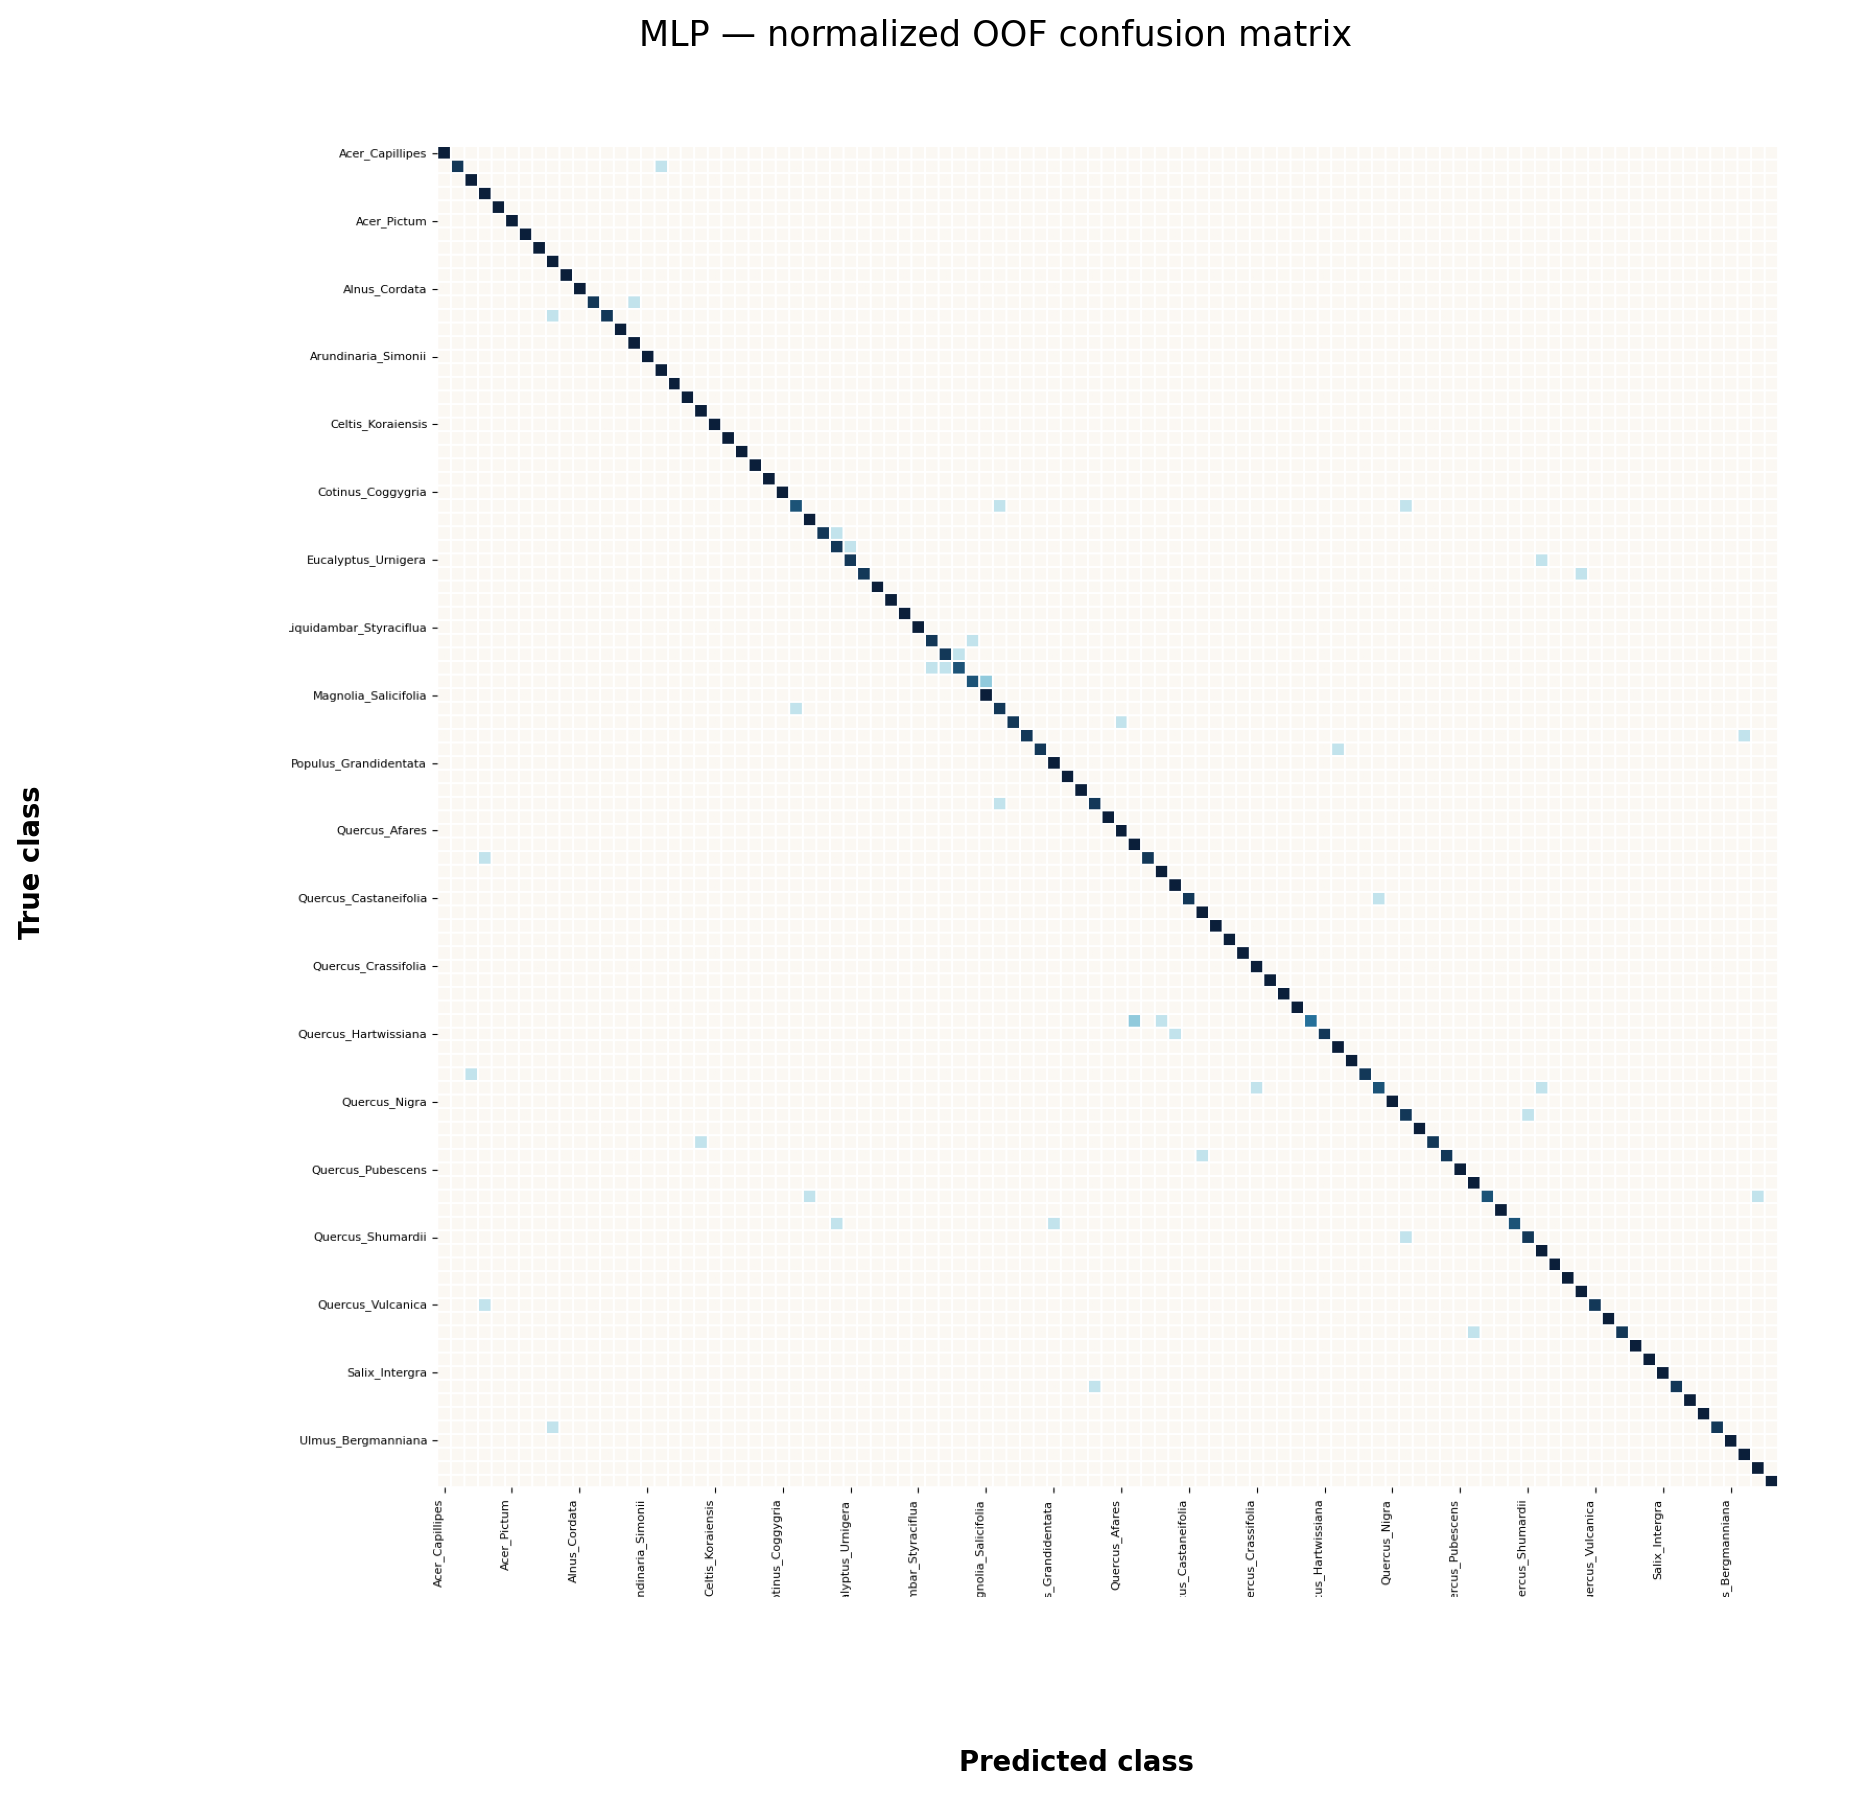
\includegraphics[width=\textwidth]{../figures/en/figA_confusion_mlp_tuned.png}
\caption{Normalized confusion matrix from the out-of-fold predictions of the \texttt{tuned} variant. Residual errors remain limited, but are more numerous than for the three best-performing families.}
\end{figure}

\begin{figure}[H]
\centering
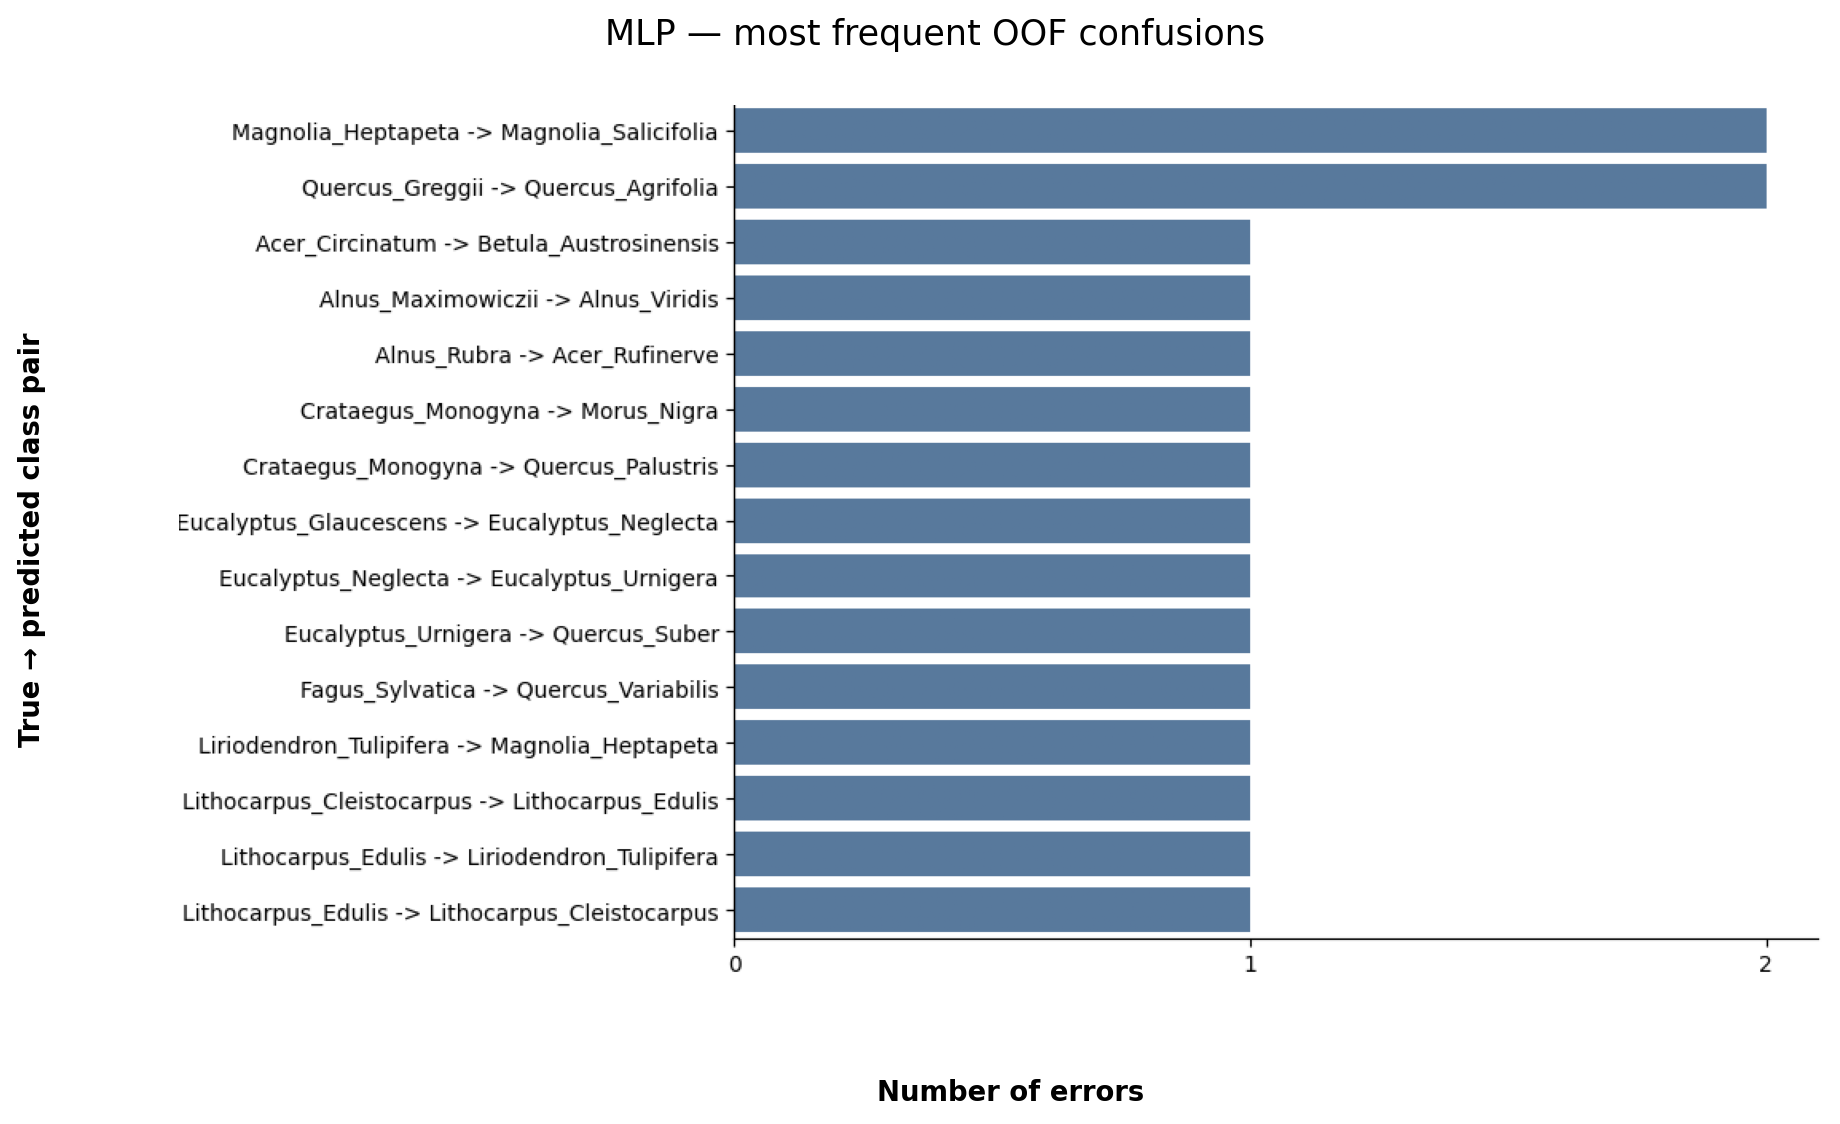
\includegraphics[width=\textwidth]{../figures/en/fig_mlp_top12_confusions.png}
\caption{Leading confusions for the tuned MLP. They remain relatively concentrated and confirm an overall competitive performance level.}
\end{figure}

\subsubsection{Secondary corroboration}
The frozen corroboration set retains \texttt{scaled\_only} as the secondary reference. On this split, the reference and \texttt{tuned} variants obtain exactly the same scores: \texttt{0.9785} in \texttt{F1-macro} and \texttt{0.9798} in \texttt{accuracy}. The \texttt{scaled\_pca} variant remains slightly behind. The \texttt{tuned - reference} delta is therefore zero.

\begin{table}[H]
\centering
\begin{tabular}{|l|r|r|l|}
\hline
\textbf{Variant} & \textbf{Corroboration F1} & \textbf{Corroboration accuracy} & \textbf{Role} \\
\hline
\texttt{default} & \texttt{0.0080} & \texttt{0.0404} & baseline \\
\texttt{scaled\_only} & \texttt{0.9785} & \texttt{0.9798} & reference \\
\texttt{scaled\_pca} & \texttt{0.9737} & \texttt{0.9747} & descriptive \\
\texttt{tuned} & \texttt{0.9785} & \texttt{0.9798} & tuned \\
\hline
\end{tabular}
\end{table}

The conclusion for the MLP remains straightforward: with appropriate preprocessing, the family becomes strong, but tuning adds no robust gain on this dataset. It remains credible without surpassing the best, more parsimonious options.

\begin{figure}[H]
\centering
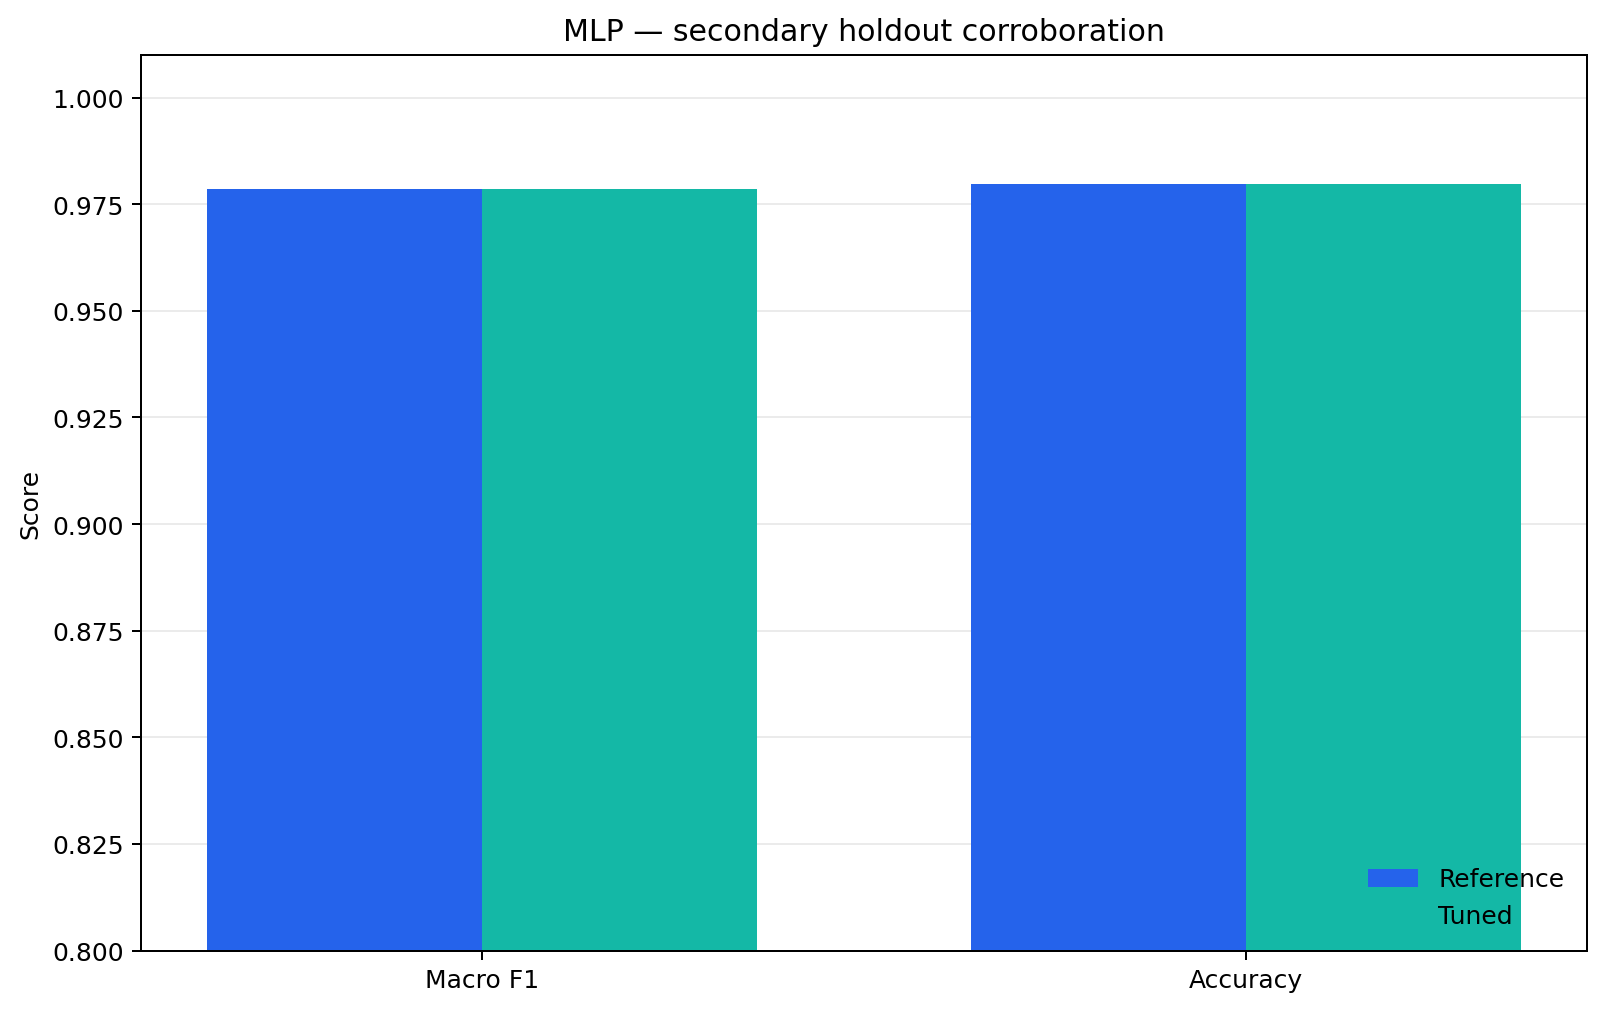
\includegraphics[width=\textwidth]{../figures/en/fig_mlp_corroboration_holdout.png}
\caption{Secondary comparison between the reference and \texttt{tuned} MLP variants on the corroboration set.}
\end{figure}

% ==========================================
% 4. OVERALL COMPARISON AND DISCUSSION
% ==========================================

\section{Global Comparison and Discussion}

The inter-model comparison presented in this section is based exclusively on the \texttt{tuned} variants evaluated through nested cross-validation. This choice limits the selection bias introduced by hyperparameter tuning, in accordance with established recommendations in the model-evaluation literature (Varma and Simon, 2006; Cawley and Talbot, 2010). The untuned variants and model-specific diagnostics retain an interpretive role, while the frozen corroboration set remains a secondary control.

\subsection{Confirmatory Inter-Model Results}
The following table compares the six model families on the basis of their confirmatory \texttt{tuned} performance, with \texttt{macro-F1} as the primary metric and \texttt{accuracy} as the secondary metric.

\begin{table}[H]
\centering
\begin{tabular}{|l|r|r|r|}
\hline
\textbf{Model} & \textbf{Macro-F1 (mean $\pm$ std)} & \textbf{Accuracy (mean $\pm$ std)} & \textbf{Time (s)} \\
\hline
Logistic regression & $0.9787 \pm 0.0198$ & $0.9848 \pm 0.0146$ & \texttt{77.05} \\
RBF SVM & $0.9756 \pm 0.0207$ & $0.9823 \pm 0.0151$ & \texttt{56.49} \\
Random forest & $0.9702 \pm 0.0140$ & $0.9747 \pm 0.0089$ & \texttt{250.11} \\
MLP & $0.9389 \pm 0.0322$ & $0.9482 \pm 0.0279$ & \texttt{38.25} \\
Perceptron & $0.8085 \pm 0.0523$ & $0.8409 \pm 0.0411$ & \texttt{29.79} \\
Decision tree & $0.4295 \pm 0.0546$ & $0.4610 \pm 0.0627$ & \texttt{11.47} \\
\hline
\end{tabular}
\caption{Confirmatory inter-model comparison}
\end{table}

\begin{figure}[H]
\centering
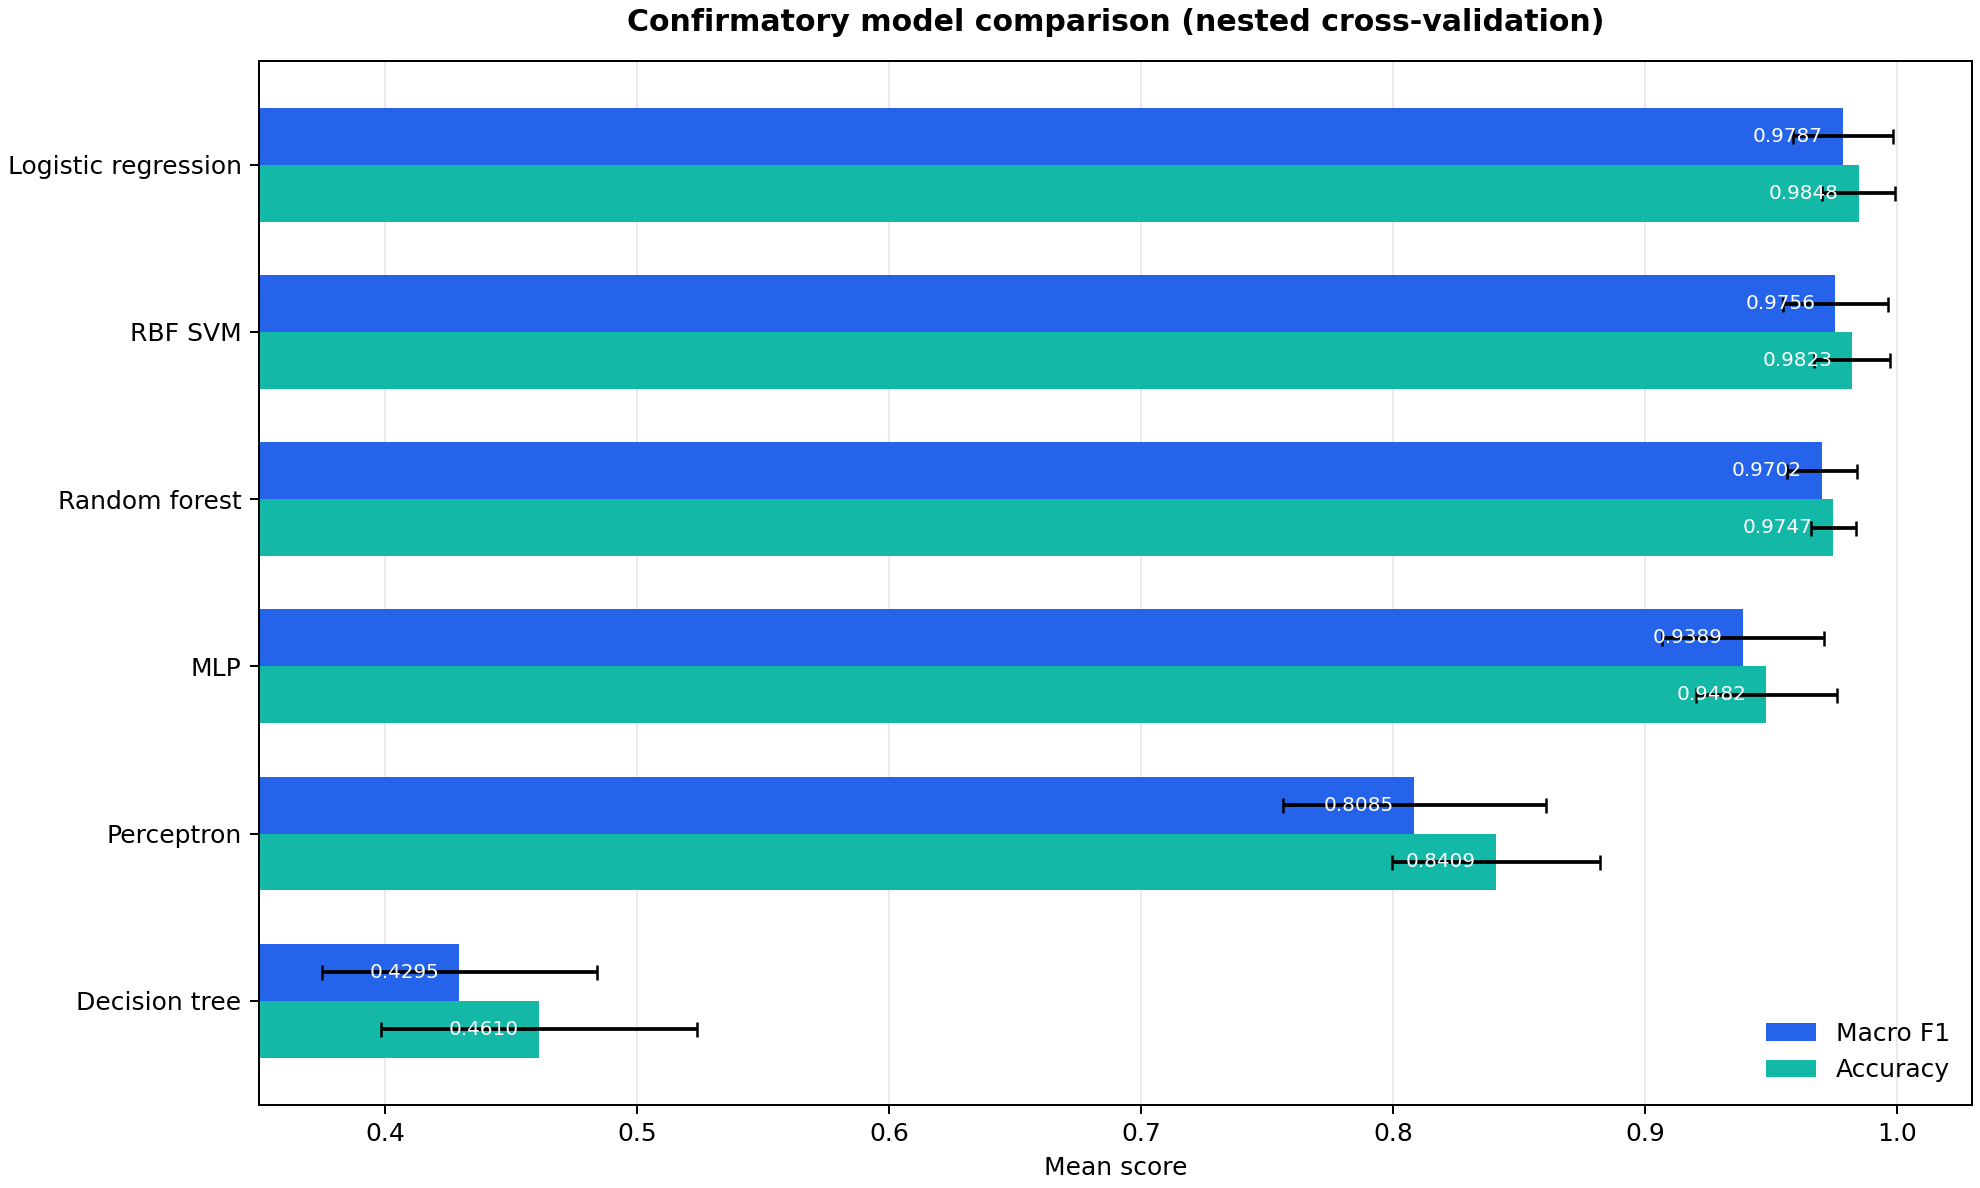
\includegraphics[width=\textwidth]{../figures/en/fig02_barplot_comparatif_tuned.png}
\caption{Confirmatory inter-model comparison}
\end{figure}

A clear hierarchy emerges. Logistic regression and the RBF SVM form the leading confirmatory pair, with a slight average advantage for logistic regression. The random forest also performs at a very high level, although it falls slightly behind. The MLP is a credible solution but does not match the top three models. The perceptron serves effectively as a linear baseline after preprocessing, whereas a single decision tree is clearly inadequate for this multiclass problem.

The key point is the proximity of logistic regression and the SVM. Their mean \texttt{macro-F1} scores differ only slightly, although logistic regression retains the higher average. In the absence of a formal statistical test between these closely matched models, it is more prudent to describe them as confirmatory co-leaders, with logistic regression leading on the mean, than to claim a single definitive winner.

\subsection{Relative Stability and Practical Trade-offs}
Cross-fold standard deviations do not constitute a statistical test, but they provide useful information about the relative stability of the model families under the selected protocol.

\begin{table}[H]
\centering
\begin{tabular}{|l|r|l|}
\hline
\textbf{Model} & \textbf{F1 range} & \textbf{Stability assessment} \\
\hline
Logistic regression & \texttt{0.0512} & Very good stability \\
RBF SVM & \texttt{0.0549} & Stability comparable to logistic regression \\
Random forest & \texttt{0.0343} & Most stable of the three leading models \\
MLP & \texttt{0.0896} & More pronounced variability \\
Perceptron & \texttt{0.1121} & Insufficient stability for a leading position \\
Decision tree & \texttt{0.1449} & Very high structural instability \\
\hline
\end{tabular}
\end{table}

\begin{figure}[H]
\centering
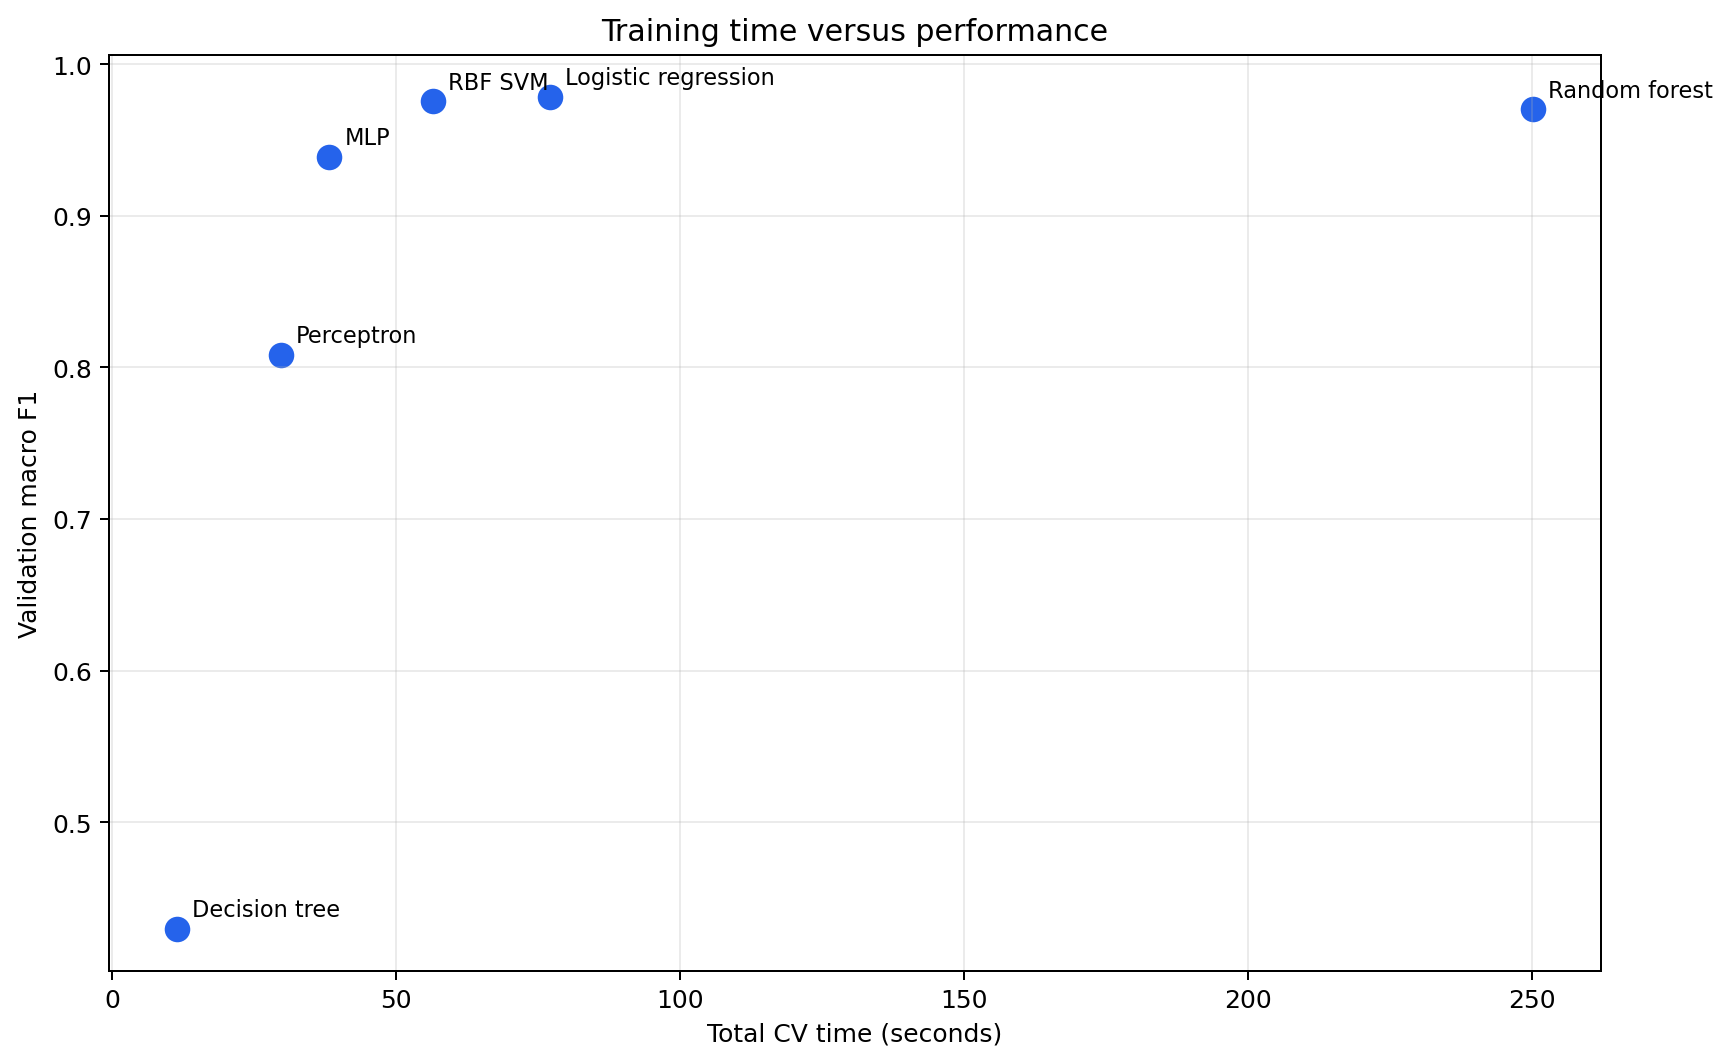
\includegraphics[width=\textwidth]{../figures/en/fig3b_temps_vs_performance.png}
\caption{Compute-time/performance trade-off}
\end{figure}

From a practical standpoint, logistic regression offers the best balance of average performance, computational cost, and interpretability. It achieves the highest observed confirmatory performance while remaining easier to interpret than an RBF SVM and far less expensive than a random forest. The SVM produces a very similar result, but with lower interpretability. The random forest confirms its robustness, although its computational cost is by far the highest among the leading models.

The MLP and perceptron are relatively fast, but that advantage does not offset their performance deficit relative to the strongest candidates. Finally, although the decision tree is inexpensive, its weak predictive performance prevents it from being a defensible solution for this project.

\subsection{Cross-Model Error Analysis}
The \texttt{tuned} OOF predictions on the development subset (\texttt{n = 792}) complement the overall analysis with a more detailed view of the number and profile of errors.

\begin{table}[H]
\centering
\begin{tabular}{|l|r|r|r|}
\hline
\textbf{Model} & \textbf{Correct predictions} & \textbf{Errors} & \textbf{Error rate} \\
\hline
Logistic regression & \texttt{780} & \texttt{12} & \texttt{1.5 \%} \\
RBF SVM & \texttt{778} & \texttt{14} & \texttt{1.8 \%} \\
Random forest & \texttt{772} & \texttt{20} & \texttt{2.5 \%} \\
MLP & \texttt{751} & \texttt{41} & \texttt{5.2 \%} \\
Perceptron & \texttt{666} & \texttt{126} & \texttt{15.9 \%} \\
Decision tree & \texttt{365} & \texttt{427} & \texttt{53.9 \%} \\
\hline
\end{tabular}
\end{table}

This perspective confirms the hierarchy observed for \texttt{macro-F1}. The two co-leaders make very few errors across the development set, the random forest remains close behind, and a more substantial gap then appears before the MLP, perceptron, and especially the decision tree. In other words, the difference between the strongest and weaker models is not limited to small score fluctuations: it corresponds to a change in the order of magnitude of the error count.

The overlap among the errors made by the three strongest models provides further insight.

\begin{table}[H]
\centering
\begin{tabular}{|l|r|r|r|}
\hline
\textbf{Comparison} & \textbf{Shared errors} & \textbf{Error union} & \textbf{Jaccard} \\
\hline
Logistic regression vs.\ SVM & \texttt{10} & \texttt{16} & \texttt{0.625} \\
Logistic regression vs.\ random forest & \texttt{5} & \texttt{27} & \texttt{0.185} \\
SVM vs.\ random forest & \texttt{5} & \texttt{29} & \texttt{0.172} \\
\hline
\end{tabular}
\end{table}

Logistic regression and the SVM therefore share a substantial portion of their residual errors. The overlap is high: 10 shared errors out of 16 distinct errors in total, yielding a Jaccard index of \texttt{0.625}. This proximity is consistent with their nearly identical performance and suggests that they exploit very similar discriminative structures. The random forest shares fewer errors with either model, supporting the idea that it has a partially different error profile without altering its slight disadvantage on the primary metric.

Overall, the cross-model error analysis suggests that the remaining gains no longer depend on coarse global separation, but on a small number of ambiguous cases. The strongest models therefore differ less in how they represent the general nature of the problem than in their ability to handle these residual decision-boundary regions.

\subsection{Secondary Corroboration on the Frozen Set}
The frozen corroboration set provides a secondary external check of the selected pipelines. It replaces neither the confirmatory logic of \texttt{nested CV} nor the hierarchy established above.

\begin{table}[H]
\centering
\begin{tabularx}{\textwidth}{|>{\raggedright\arraybackslash}p{3.0cm}|>{\centering\arraybackslash}p{2.8cm}|>{\centering\arraybackslash}p{2.2cm}|>{\centering\arraybackslash}p{2.2cm}|Y|}
\hline
\textbf{Model} & \textbf{Reference variant} & \textbf{Reference corroboration F1} & \textbf{Tuned corroboration F1} & \textbf{Assessment} \\
\hline
Logistic regression & \texttt{scaled\_only} & \texttt{0.9892} & \texttt{0.9892} & Neutral tuning effect on corroboration \\
RBF SVM & \texttt{scaled\_only} & \texttt{0.9838} & \texttt{0.9946} & Favorable tuning effect on corroboration \\
Random forest & \texttt{default} & \texttt{0.9842} & \texttt{0.9842} & Neutral tuning effect on corroboration \\
MLP & \texttt{scaled\_only} & \texttt{0.9785} & \texttt{0.9785} & Neutral tuning effect on corroboration \\
Perceptron & \texttt{scaled\_only} & \texttt{0.8815} & \texttt{0.8694} & Slightly unfavorable tuning effect on corroboration \\
\hline
\end{tabularx}
\end{table}

\begin{figure}[H]
\centering
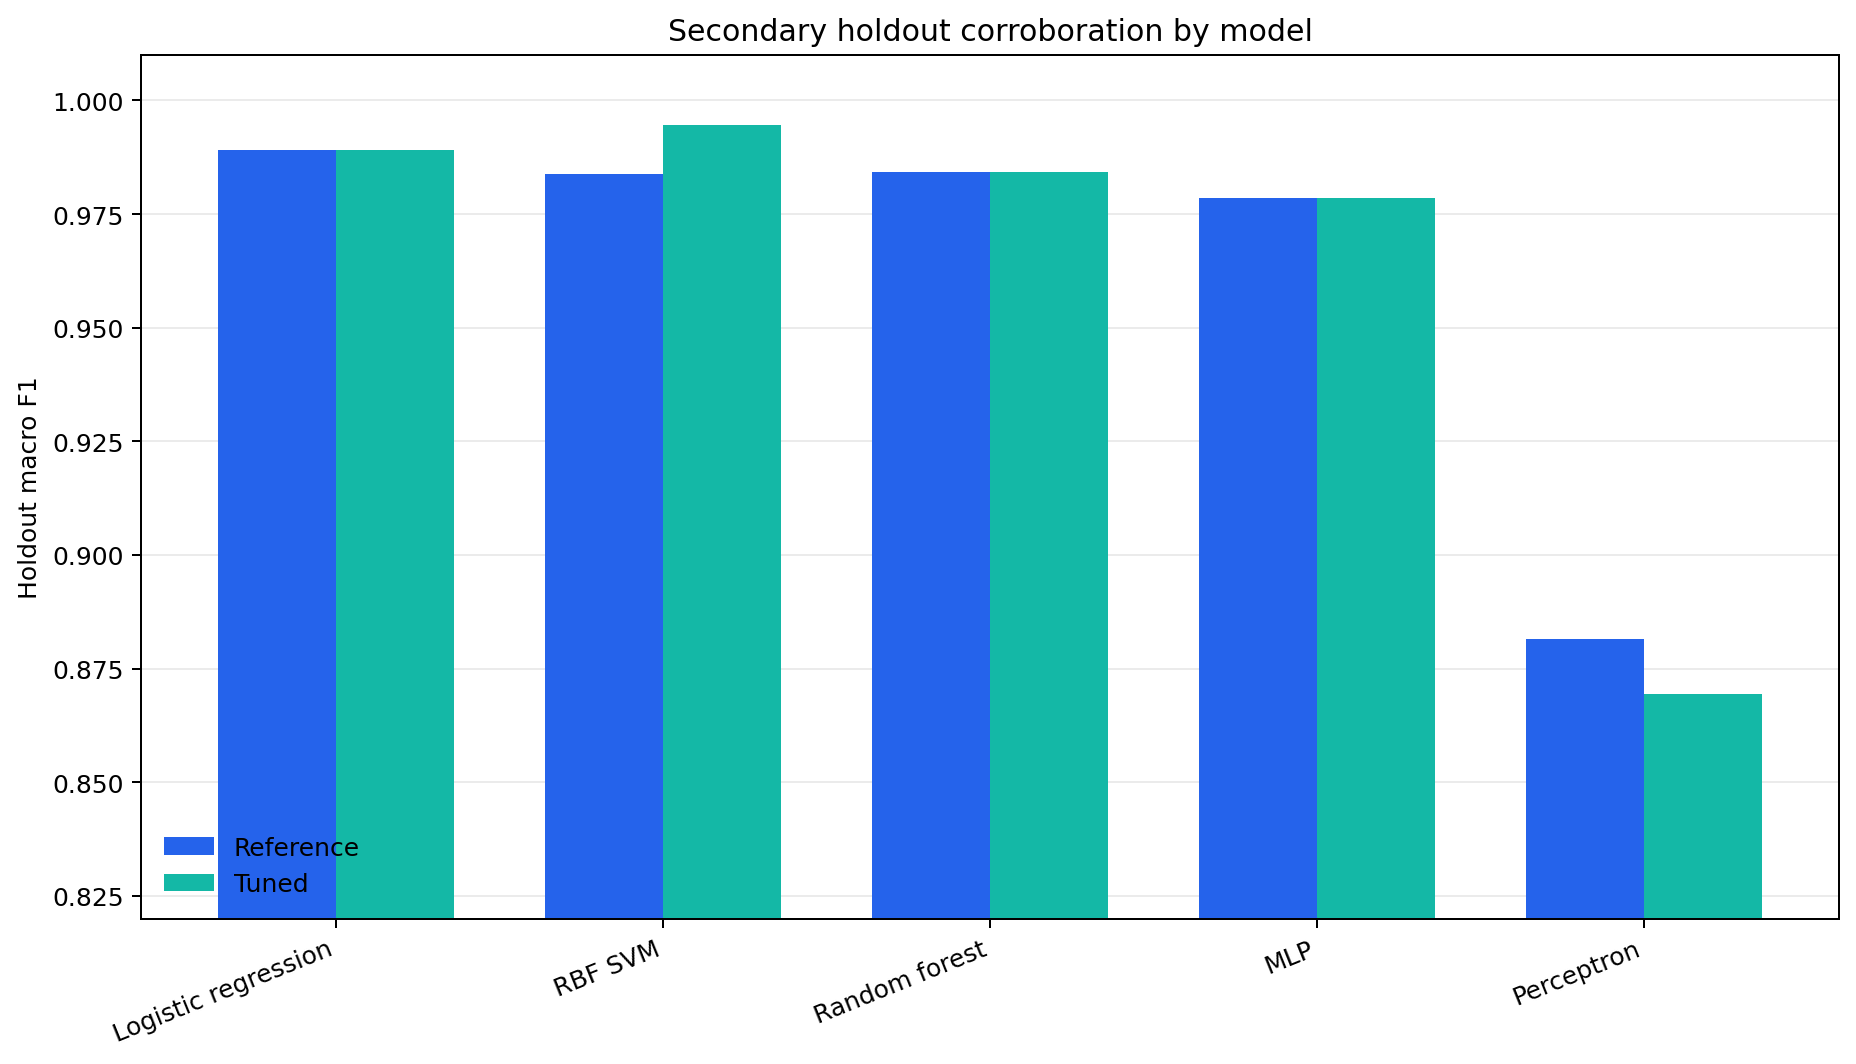
\includegraphics[width=\textwidth]{../figures/en/fig_global_corroboration_holdout.png}
\caption{For each eligible model, comparison of the reference variant selected on the development set with the \texttt{tuned} variant on the frozen corroboration set.}
\end{figure}

Considered in isolation, these figures might suggest reranking some models. Such an interpretation would be methodologically unsound. The corroboration set does not represent a new selection stage here, but rather a final secondary check on a single split. It broadly confirms the strength of the leading pipelines, but it should not be used to overturn the primary hierarchy based on confirmatory nested cross-validation estimates.

\subsection{Scientific Discussion}
Several general lessons emerge from the study. First, a well-regularized linear model can remain extremely competitive in a high-dimensional multiclass problem when paired with suitable preprocessing. Logistic regression shows that a relatively parsimonious structure can be sufficient to achieve a very high level of generalization.

Second, the RBF SVM confirms the presence of exploitable nonlinear structure, but provides no measurable improvement over logistic regression. In this context, practical criteria---particularly interpretability and computational cost---can therefore guide the choice between the two.

Third, the random forest also warrants attention. Its very strong performance without scaling shows that an aggregated tree-based approach can capture the problem structure effectively. However, its substantial additional cost and slight deficit in \texttt{macro-F1} make it a less natural choice when the objective is the best overall trade-off.

The MLP results are also instructive. The model becomes competitive after normalization, but it does not outperform the strongest, simpler approaches. This observation is consistent with a dataset that is relatively modest in size given the multiclass complexity of the problem: greater representational capacity does not automatically yield better generalization.

Finally, the contrast between the decision tree and random forest underscores the decisive role of aggregation. The interpretability of a single tree is not enough when the model's variance becomes excessive. Here, the individual tree primarily serves as a useful counterpoint that illustrates what the ensemble corrects.

In summary, the project demonstrates above all that a well-regularized linear model can remain highly competitive when supported by appropriate preprocessing. The gains from more flexible models are modest here and must be assessed in light of their cost, stability, and interpretability.

% ==========================================
% 5. CONCLUSION
% ==========================================

\section{Conclusion}

This study compared six model families on the \texttt{Leaf Classification} dataset within a framework that explicitly separates exploration, confirmation, and secondary corroboration. The primary ranking is based on the \texttt{tuned} variants evaluated through nested cross-validation, with \texttt{macro-F1} as the reference metric.

The results confirm a leading pair consisting of logistic regression and the RBF SVM, with a slight average advantage for logistic regression and the random forest close behind. The MLP remains credible without matching this trio, while the perceptron and especially the decision tree lag behind.

From a practical standpoint, logistic regression is the most defensible choice because it combines the highest observed mean score, moderate computational cost, and greater interpretability than the closest nonlinear alternatives. The frozen corroboration set broadly supports this interpretation without redefining it.

This conclusion is nevertheless context-specific: it is based on a single dataset, without independent external validation, and on one nested cross-validation scheme. The most natural extensions are therefore to repeat the evaluation across multiple data splits, test the robustness of the conclusions on external data, and examine in greater depth the residual errors shared by the strongest models.

% ==========================================
% 6. APPENDICES
% ==========================================

\section{Appendices}

\subsection{Purpose and Use of the Appendices}
The appendices bring together material that supports reproducibility, methodological auditing, and detailed examination of the artifacts without overloading the main body of the report. They extend the analysis without shifting its inferential basis. The principal conclusions remain grounded in the \texttt{tuned} variants evaluated with \texttt{nested\_cv}; depending on the case, the other information retained here is descriptive, exploratory, or documentary.

\subsection{Detailed Protocol and Canonical Artifacts}

\begin{table}[H]
\centering
\begin{tabular}{|l|l|}
\hline
\textbf{Element} & \textbf{Selected value} \\
\hline
Global seed & \texttt{42} \\
Frozen split & \texttt{80 \%} development / \texttt{20 \%} corroboration \\
Development set size & \texttt{792} \\
Corroboration set size & \texttt{198} \\
Primary cross-validation & \texttt{5} outer folds \\
Internal tuning & \texttt{3} folds \\
Variance retained by \texttt{PCA} & \texttt{0.99} \\
Primary metric & \texttt{Macro-F1} \\
Secondary metric & \texttt{Accuracy} \\
CV parallelism & \texttt{CV\_N\_JOBS = 1} \\
\hline
\end{tabular}
\caption{Experimental protocol parameters}
\end{table}

Preserving a frozen split separate from the development subset maintains a clear distinction between the primary analysis and secondary corroboration. The non-\texttt{tuned} variants are used to explore the effects of preprocessing and model capacity; only the \texttt{tuned} variants form the basis of the inter-model ranking.

\subsection{Detailed Results by Variant}

\begin{table}[H]
\centering
\begin{tabular}{|l|l|l|r|r|r|}
\hline
\textbf{Model} & \textbf{Variant} & \textbf{Status} & \textbf{Validation macro-F1} & \textbf{Validation accuracy} & \textbf{Time (s)} \\
\hline
\texttt{perceptron} & \texttt{default} & Exploratory & \texttt{0.6979} & \texttt{0.7436} & \texttt{0.62} \\
\texttt{perceptron} & \texttt{scaled\_only} & Exploratory & \texttt{0.8228} & \texttt{0.8460} & \texttt{0.60} \\
\texttt{perceptron} & \texttt{scaled\_pca} & Exploratory & \texttt{0.8057} & \texttt{0.8346} & \texttt{0.65} \\
\texttt{perceptron} & \texttt{tuned} & Confirmatory & \texttt{0.8085} & \texttt{0.8409} & \texttt{29.79} \\
\texttt{regression\_logistique} & \texttt{default} & Exploratory & \texttt{0.2591} & \texttt{0.3106} & \texttt{1.69} \\
\texttt{regression\_logistique} & \texttt{scaled\_only} & Exploratory & \texttt{0.9798} & \texttt{0.9861} & \texttt{8.10} \\
\texttt{regression\_logistique} & \texttt{scaled\_pca} & Exploratory & \texttt{0.9784} & \texttt{0.9848} & \texttt{2.21} \\
\texttt{regression\_logistique} & \texttt{tuned} & Confirmatory & \texttt{0.9787} & \texttt{0.9848} & \texttt{77.05} \\
\texttt{svm} & \texttt{default} & Exploratory & \texttt{0.8389} & \texttt{0.8561} & \texttt{2.36} \\
\texttt{svm} & \texttt{scaled\_only} & Exploratory & \texttt{0.9712} & \texttt{0.9785} & \texttt{2.45} \\
\texttt{svm} & \texttt{scaled\_pca} & Exploratory & \texttt{0.9712} & \texttt{0.9785} & \texttt{2.50} \\
\texttt{svm} & \texttt{tuned} & Confirmatory & \texttt{0.9756} & \texttt{0.9823} & \texttt{56.49} \\
\texttt{foret\_aleatoire} & \texttt{default} & Exploratory & \texttt{0.9764} & \texttt{0.9785} & \texttt{9.16} \\
\texttt{foret\_aleatoire} & \texttt{restricted\_depth} & Exploratory & \texttt{0.9345} & \texttt{0.9445} & \texttt{5.42} \\
\texttt{foret\_aleatoire} & \texttt{tuned} & Confirmatory & \texttt{0.9702} & \texttt{0.9747} & \texttt{250.11} \\
\texttt{arbre\_decision} & \texttt{default} & Exploratory & \texttt{0.5809} & \texttt{0.6174} & \texttt{1.04} \\
\texttt{arbre\_decision} & \texttt{restricted\_depth} & Exploratory & \texttt{0.1468} & \texttt{0.1529} & \texttt{0.56} \\
\texttt{arbre\_decision} & \texttt{tuned} & Confirmatory & \texttt{0.4295} & \texttt{0.4610} & \texttt{11.47} \\
\texttt{mlp} & \texttt{default} & Exploratory & \texttt{0.1642} & \texttt{0.1863} & \texttt{1.97} \\
\texttt{mlp} & \texttt{scaled\_only} & Exploratory & \texttt{0.9389} & \texttt{0.9482} & \texttt{2.01} \\
\texttt{mlp} & \texttt{scaled\_pca} & Exploratory & \texttt{0.9323} & \texttt{0.9444} & \texttt{1.97} \\
\texttt{mlp} & \texttt{tuned} & Confirmatory & \texttt{0.9389} & \texttt{0.9482} & \texttt{38.25} \\
\hline
\end{tabular}
\caption{Validation results by variant}
\end{table}

This table must be read with due regard for the status of each row. Scores for the exploratory variants document the effects of preprocessing and complexity; they must not be conflated with the confirmatory scores of the \texttt{tuned} variants.

\subsection{Hyperparameters Selected by Outer Fold}
The stability of fold-level selection provides useful evidence about the robustness of the model families. Some families converge on the same settings in nearly every fold, while others show more pronounced variability, particularly in the use of \texttt{PCA} or the strength of regularization.

\begin{table}[H]
\centering
\begin{tabular}{|l|>{\raggedright\arraybackslash}p{10.5cm}|}
\hline
\textbf{Model} & \textbf{Patterns observed across the 5 outer folds} \\
\hline
\texttt{perceptron} & \texttt{alpha = 0.001}, \texttt{penalty = l1} in every fold; \texttt{PCA} selected once, otherwise \texttt{passthrough} \\
\hline
\texttt{regression\_logistique} & \texttt{C} alternates between \texttt{1.0} and \texttt{10.0}; \texttt{PCA} selected in one fold, otherwise \texttt{passthrough} \\
\hline
\texttt{svm} & \texttt{C = 10.0} and \texttt{gamma = scale} in every fold; \texttt{PCA} selected once \\
\hline
\texttt{foret\_aleatoire} & Nearly perfectly stable settings: \texttt{max\_depth = None}, \texttt{max\_features = sqrt}, \texttt{min\_samples\_leaf = 1}, and \texttt{n\_estimators = 400} in every fold \\
\hline
\texttt{arbre\_decision} & \texttt{max\_depth = 20}, \texttt{criterion = gini}, and \texttt{min\_samples\_leaf = 1}; only \texttt{ccp\_alpha} varies, taking \texttt{0.005} in one fold and \texttt{0.0} otherwise \\
\hline
\texttt{mlp} & \texttt{hidden\_layer\_sizes = [128]} in every fold; \texttt{alpha = 0.0001} in four folds and \texttt{0.001} in one fold; \texttt{PCA} is never selected \\
\hline
\end{tabular}
\caption{Hyperparameters selected by outer fold}
\end{table}

The random forest, SVM, and MLP show highly consistent fold-level selection. Logistic regression and the perceptron remain more sensitive to linear regularization and the possible selection of \texttt{PCA}, but this variability does not alter their overall interpretation. For the decision tree, stability in the selected depth does not offset the predictive instability observed in its scores.

\subsection{AI Use Declaration}
This declaration is provided for documentary transparency. AI assistance was used on a limited basis during the project, but it did not replace scientific decision-making, the execution of experiments, or the final validation of results.

\paragraph{Where AI was used}
\begin{itemize}
    \item assistance with structuring Markdown and LaTeX documents;
    \item occasional assistance with repository cleanup, reorganization, and documentation;
    \item technical assistance with certain adjustments to code, scripts, and notebooks;
    \item proposals or initial generation of some code sections, which were subsequently reviewed, modified, tested, and validated by a human before being retained.
\end{itemize}

\paragraph{Work performed manually}
\begin{itemize}
    \item definition of the topic, objectives, and experimental protocol;
    \item selection of the models, variants, metrics, and evaluation framework;
    \item execution of the experiments, notebooks, and pipeline;
    \item review, correction, and validation of the retained code;
    \item verification of the numerical results, figures, and their consistency;
    \item selection of the material included in the final report;
    \item scientific interpretation of the results and final writing validated by a human.
\end{itemize}

% ==========================================
% 7. BIBLIOGRAPHY
% ==========================================

\section{Bibliography}
\sloppy

\begin{itemize}
    \item Breiman, L. (2001). \emph{Random forests}. \emph{Machine Learning, 45}(1), 5-32. \url{https://doi.org/10.1023/A:1010933404324}
    \item Cawley, G. C., \& Talbot, N. L. C. (2010). \emph{On over-fitting in model selection and subsequent selection bias in performance evaluation}. \emph{Journal of Machine Learning Research, 11}, 2079-2107.
    \item Kaggle. (n.d.). \emph{Leaf Classification}. \url{https://www.kaggle.com/c/leaf-classification}
    \item LeCun, Y., Bottou, L., Orr, G. B., \& Muller, K.-R. (1998). \emph{Efficient backprop}. In G. B. Orr \& K.-R. Muller (Eds.), \emph{Neural networks: Tricks of the trade} (pp. 9-50). Springer.
    \item Niculescu-Mizil, A., \& Caruana, R. (2005). \emph{Predicting good probabilities with supervised learning}. In \emph{Proceedings of the 22nd International Conference on Machine Learning} (pp. 625-632).
    \item Platt, J. (1999). \emph{Probabilistic outputs for support vector machines and comparisons to regularized likelihood methods}. In A. J. Smola, P. Bartlett, B. Scholkopf, \& D. Schuurmans (Eds.), \emph{Advances in large margin classifiers} (pp. 61-74). MIT Press.
    \item scikit-learn developers. (n.d.). \emph{DecisionTreeClassifier}. \url{https://scikit-learn.org/stable/modules/generated/sklearn.tree.DecisionTreeClassifier.html}
    \item scikit-learn developers. (n.d.). \emph{F1 score}. \url{https://scikit-learn.org/stable/modules/generated/sklearn.metrics.f1_score.html}
    \item scikit-learn developers. (n.d.). \emph{Importance of feature scaling}. \url{https://scikit-learn.org/stable/auto_examples/preprocessing/plot_scaling_importance.html}
    \item scikit-learn developers. (n.d.). \emph{LogisticRegression}. \url{https://scikit-learn.org/stable/modules/generated/sklearn.linear_model.LogisticRegression.html}
    \item scikit-learn developers. (n.d.). \emph{MLPClassifier}. \url{https://scikit-learn.org/stable/modules/generated/sklearn.neural_network.MLPClassifier.html}
    \item scikit-learn developers. (n.d.). \emph{Model evaluation: Quantifying the quality of predictions}. \url{https://scikit-learn.org/stable/modules/model_evaluation.html}
    \item scikit-learn developers. (n.d.). \emph{Nested versus non-nested cross-validation}. \url{https://scikit-learn.org/stable/auto_examples/model_selection/plot_nested_cross_validation_iris.html}
    \item scikit-learn developers. (n.d.). \emph{PCA}. \url{https://scikit-learn.org/stable/modules/generated/sklearn.decomposition.PCA.html}
    \item scikit-learn developers. (n.d.). \emph{Perceptron}. \url{https://scikit-learn.org/stable/modules/generated/sklearn.linear_model.Perceptron.html}
    \item scikit-learn developers. (n.d.). \emph{Probability calibration}. \url{https://scikit-learn.org/stable/modules/calibration.html}
    \item scikit-learn developers. (n.d.). \emph{RandomForestClassifier}. \url{https://scikit-learn.org/stable/modules/generated/sklearn.ensemble.RandomForestClassifier.html}
    \item scikit-learn developers. (n.d.). \emph{StandardScaler}. \url{https://scikit-learn.org/stable/modules/generated/sklearn.preprocessing.StandardScaler.html}
    \item scikit-learn developers. (n.d.). \emph{SVC}. \url{https://scikit-learn.org/stable/modules/generated/sklearn.svm.SVC.html}
    \item Varma, S., \& Simon, R. (2006). \emph{Bias in error estimation when using cross-validation for model selection}. \emph{BMC Bioinformatics, 7}, Article 91.\\ \url{https://doi.org/10.1186/1471-2105-7-91}
\end{itemize}

\end{document}
